% !TEX encoding = UTF-8 Unicode
\documentclass{dissert}


\bibliographystyle{unsrt}

% В этом документе преамбула

%%% Работа с русским языком
\usepackage{cmap}					% поиск в PDF
\usepackage{mathtext} 				% русские буквы в формулах
\usepackage[T2A]{fontenc}			% кодировка
\usepackage[utf8]{inputenc}			% кодировка исходного текста
\usepackage[english,russian]{babel}% локализация и переносы
\usepackage{indentfirst}
\usepackage{hyperref}
\frenchspacing

\renewcommand{\epsilon}{\ensuremath{\varepsilon}}
\renewcommand{\phi}{\ensuremath{\varphi}}
\renewcommand{\kappa}{\ensuremath{\varkappa}}
\renewcommand{\le}{\ensuremath{\leqslant}}
\renewcommand{\leq}{\ensuremath{\leqslant}}
\renewcommand{\ge}{\ensuremath{\geqslant}}
\renewcommand{\geq}{\ensuremath{\geqslant}}
\renewcommand{\emptyset}{\varnothing}

%%% Дополнительная работа с математикой
\usepackage{amsmath,amsfonts,amssymb,amsthm,mathtools} % AMS
\usepackage{icomma} % "Умная" запятая: $0,2$ --- число, $0, 2$ --- перечисление

%% Номера формул
%\mathtoolsset{showonlyrefs=true} % Показывать номера только у тех формул, на которые есть \eqref{} в тексте.
%\usepackage{leqno} % Нумереация формул слева

%% Свои команды
\DeclareMathOperator{\sgn}{\mathop{sgn}}

%% Перенос знаков в формулах (по Львовскому)
\newcommand*{\hm}[1]{#1\nobreak\discretionary{}
	{\hbox{$\mathsurround=0pt #1$}}{}}

%%% Работа с картинками
\usepackage{graphicx}  % Для вставки рисунков
\setlength\fboxsep{3pt} % Отступ рамки \fbox{} от рисунка
\setlength\fboxrule{1pt} % Толщина линий рамки \fbox{}
\usepackage{wrapfig} % Обтекание рисунков текстом
\usepackage{subfig}

%%% Работа с таблицами
\usepackage{array,tabularx,tabulary,booktabs} % Дополнительная работа с таблицами
\usepackage{longtable}  % Длинные таблицы
\usepackage{multirow} % Слияние строк в таблице
\usepackage{xcolor}

\usepackage{geometry}
\geometry{left=2.5cm}
\geometry{right=1.0cm}
\geometry{top=2.0cm}
\geometry{bottom=2.0cm}

%\def\BibUrl#1.{}
%\bibliographystyle{gost2008} 
\theoremstyle{definition}
\newtheorem{theorem}{Теорема}
\newtheorem{lemma}{Лемма}
\newtheorem{definition}{Определение}
\newtheorem{statement}{Утверждение}

\renewcommand{\contentsname}{Содержание}
\renewcommand{\contentsdesc}{Стр.}
\renewcommand{\chaptername}{Глава}

%%% Библиография %%%
\makeatletter
\bibliographystyle{utf8gost71u}     % Оформляем библиографию по ГОСТ 7.1 (ГОСТ Р 7.0.11-2011, 5.6.7)
%\renewcommand{\@biblabel}[1]{#1.}   % Заменяем библиографию с квадратных скобок на точку
\makeatother

\usepackage{algorithm}
\usepackage[noend]{algcompatible}
\def\algorithmicrequire{\textbf{Вход:}}
\def\algorithmicensure{\textbf{Выход:}}
\def\algorithmicif{\textbf{если}}
\def\algorithmicthen{\textbf{то}}
\def\algorithmicelse{\textbf{иначе}}
\def\algorithmicelsif{\textbf{иначе если}}
\def\algorithmicfor{\textbf{для}}
\def\algorithmicforall{\textbf{для всех}}
\def\algorithmicdo{}
\def\algorithmicand{\textbf{и}}
\def\algorithmicwhile{\textbf{пока}}
\def\algorithmicrepeat{\textbf{повторять}}
\def\algorithmicuntil{\textbf{пока}}
\def\algorithmicloop{\textbf{цикл}}
\def\algorithmiccomment#1{\quad// {\sl #1}}


\newcommand{\ba}{\mathbf{a}}
\newcommand{\bb}{\mathbf{b}}
\newcommand{\bc}{\mathbf{c}}
\newcommand{\bp}{\mathbf{p}}
\newcommand{\bq}{\mathbf{q}}
\newcommand{\bt}{\mathbf{t}}
\newcommand{\bu}{\mathbf{u}}
\newcommand{\bw}{\mathbf{w}}
\newcommand{\bx}{\mathbf{x}}
\newcommand{\by}{\mathbf{y}}
\newcommand{\bz}{\mathbf{z}}
\newcommand{\bB}{\mathbf{B}}
\newcommand{\bC}{\mathbf{C}}
\newcommand{\bE}{\mathbf{E}}
\newcommand{\bF}{\mathbf{F}}
\newcommand{\bH}{\mathbf{H}}
\newcommand{\bJ}{\mathbf{J}}
\newcommand{\bP}{\mathbf{P}}
\newcommand{\bQ}{\mathbf{Q}}
\newcommand{\bR}{\mathbf{R}}
\newcommand{\bT}{\mathbf{T}}
\newcommand{\bU}{\mathbf{U}}
\newcommand{\bW}{\mathbf{W}}
\newcommand{\bX}{\mathbf{X}}
\newcommand{\bY}{\mathbf{Y}}

\newcommand{\bbR}{\mathbb{R}}
\newcommand{\bbY}{\mathbb{Y}}

\newcommand{\cA}{\mathcal{A}}
\newcommand{\cL}{\mathcal{L}}

\newcommand{\bchi}{\boldsymbol{\chi}}
\newcommand{\bnu}{\boldsymbol{\nu}}
\newcommand{\bmu}{\boldsymbol{\mu}}
\newcommand{\btheta}{\boldsymbol{\theta}}
\newcommand{\bTheta}{\boldsymbol{\Theta}}

\newcommand{\T}{^{\text{\tiny\sffamily\upshape\mdseries T}}}

\newcommand{\bOne}{\boldsymbol{1}}
\newcommand{\bZero}{\boldsymbol{0}}
\newcommand{\argmin}{\mathop{\arg \min}\limits}
\newcommand{\argmax}{\mathop{\arg \max}\limits}


\begin{document}

\begin{titlepage}
%\begin{center}
%\textsc{МОСКОВСКИЙ ФИЗИКО-ТЕХНИЧЕСКИЙ ИНСТИТУТ (ГОСУДАРСТВЕННЫЙ УНИВЕРСИТЕТ)}\\
%\end{center}
%\vspace{1.5cm}
\begin{flushright}
{На правах рукописи}
\end{flushright}
\vspace{1.5cm}
\begin{center}
{Кузнецов Михаил Павлович}
\par
\vspace{2cm}
\textsc{ПОСТРОЕНИЕ МОДЕЛЕЙ ОБУЧЕНИЯ ПО ПРЕДПОЧТЕНИЯМ \\
        С ИСПОЛЬЗОВАНИЕМ ПОРЯДКОВЫХ ЭКСПЕРТНЫХ ОЦЕНОК}
\par
\vspace{2cm}
{05.13.18~--- Математическое моделирование, численные методы и комплексы программ}
\par
\vspace{2cm}
{Диссертация на соискание ученой степени\\
кандидата физико-математических наук}
\end{center}
\par
\vspace{3.5cm}
\begin{center}
{Москва~--- 2016}
\end{center}
\end{titlepage}




\newpage{}
\tableofcontents{}

\newpage{}
\addcontentsline{toc}{section}{Введение}
\chapter*{Введение}

Диссертационная работа посвящена построению математических моделей машинного обучения в пространствах высокой размерности.
Разработанные методы учитывают зависимости, имеющиеся в исходных данных, с целью построения простой и устойчивой модели.

\textbf{Актуальность темы.} 
В работе решается задача декодирования сигналов. 
Процесс декодирования заключается в восстановлении зависимости между двумя гетерогенными наборами данных.
Модель предсказывает отклик на входной исходный сигнал.
При построении модели возникает задача построения признакового пространства. 

Исследуется проблема избыточного исходного описания данных. 
Исходное признаковое пространство является мультикоррелированным.
При высокой мультикорреляции финальная прогностическая модель оказывается неустойчивой.
Для построения простой, устойчивой модели применяются методы снижения размерности пространства~\cite{motrenko2018multi,chun2010sparse,mehmood2012review}  и выбора признаков~\cite{katrutsa2017comprehensive,li2017feature}.

В работе рассматривается задача с векторной целевой переменной. 
Пространство целевых сигналов обладает избыточной размерностью. 
Методы снижения размерности, не учитывающие зависимости в целевом пространстве, являются не адекватными.
При предсказании векторной целевой переменной анализируется структура целевого пространства.
Предложены методы, которые учитывают зависимости как в пространстве исходных объектов, так и в пространстве целевой переменной.
Предлагается отобразить пространства исходных и целевых сигналов в скрытые подпространства меньшей размерности.
Для построения оптимальной модели предлагаются методы согласования скрытых пространств~\cite{wold1975path,rosipal2005overview,eliseyev2017recursive}.
Предложенные методы позволяют учесть регрессионную компоненту между исходным и целевым сигналами, а также авторегрессионную компоненту целевого сигнала.

Методы снижения размерности пространства понижают размерность исходного пространства объектов, и, как следствие, сложность модели существенно снижается~\cite{tipping1999probabilisticpca,wold1975path,hotelling1992relations}. 
Алгоритмы снижения размерности находят оптимальные комбинации исходных признаков. 
Если число таких комбинаций существенно меньше, чем число исходных признаков, то полученное представление снижает размерность.
Цель снижения размерности~--- получение наиболее репрезентативных и информативных комбинаций признаков для решения задачи.

Выбор признаков является частным случаем снижения размерности пространства~\cite{katrutsa2017comprehensive,katrutsa2015stress}. 
Найденные комбинации признаков являются подмножеством исходных признаков.
Таким образом отсеиваются шумовые неинформативные признаки.
Рассматриваются два типа методов выбора признаков~\cite{li2017feature,rodriguez2010quadratic,friedman2001elements}.
Первый тип методов не зависит от последующей прогностической модели.
Признаки отбираются на основе свойств исходных пространств, а не на основе свойств модели.
Второй тип методов отбирает признаки с учётом знания о прогностической модели. 

После нахождения оптимального представления данных с помощью снижения размерности, ставится задача нахождения оптимальной метрики в скрытом пространстве объектов~\cite{wang2017deep,davis2007information,kulis2012metric,yang2006distance,weinberger2009distance}.
В случае евклидова пространства естественным выбором метрики оказывается квадратичная норма.
Задача метрического обучения заключается в нахождении оптимальной метрики, связывающей объекты.

В качестве прикладной задачи анализируется задача построения нейрокомпьютерного интерфейса~\cite{wolpaw2000brain,allison2007brain}. 
Цель состоит в извлечении информации из сигналов мозговой активности~\cite{nagel2018modelling,zhang2020survey,chiarelli2018deep}. 
В качестве исходных сигналов выступают сигналы электроэнцефалограммы или электрокортикограммы. 
Целевым сигналом является траектория движения конечности индивидуума.
Задача модели построить адекватную и эффективную модель декодирования исходного сигнала в целевой сигнал.
Пространство частотных характеристик мозговых сигналов и авторегрессионное пространство целевых сигналов являются чрезвычайно избыточными~\cite{eliseyev2013recursive,eliseyev2011iterative}. 
Построение модели без учёта имеющихся зависимостей приводит к неустойчивости модели.

В диссертации решается задача декодирования с векторной целевой переменной. 
Для построения оптимальной модели декодирования сигналов предлагаются методы выбора согласованных моделей с проекцией в скрытое пространство.
Исходные и целевые сигналы проецируются в пространство существенно меньшей размерности. 
Для связи проекций исходного и целевого сигнала предлагаются методы согласования.
Рассматриваются гетерогенные наборы сигналов, природа источников измерений различны.
Рассматриваются как линейные методы декодирования, так и их нелинейные обобщения.
Доказаны теоремы об оптимальности предложенных методов выбора моделей.

\vspace{0.5cm}
\textbf{Цели работы.}
\begin{enumerate}
	\item Исследовать свойства решения задачи декодирования сигналов с векторной целевой переменной.
	\item Предложить методы снижения размерности пространства, учитывающие зависимости как в пространстве исходных сигналов, так и в целевом пространстве.
	\item Предложить процедуру выбора признаков для задачи декодирования сигналов.
	\item Исследовать свойства линейных и нелинейных моделей для решения поставленной модели. Получить теоретические оценки оптимальности моделей.
	\item Провести вычислительные эксперименты для проверки адекватности предложенных методов.
\end{enumerate}


\vspace{0.5cm}
\textbf{Основные положения, выносимые на защиту.}
\begin{enumerate}
	\item Исследована проблема снижения размерности сигналов в коррелированных пространствах высокой размерности. Предложены методы декодирования сигналов, учитывающие зависимости как в исходном, так и в целевом пространстве сигналов.
	\item Доказаны теоремы об оптимальности предлагаемых методов декодирования сигналов. Предлагаемые методы выбирают согласованные модели в случае избыточной размерности описания данных.
	\item Предложены методы выбора признаков, учитывающие зависимости как в исходном, так и в целевом пространстве. Предложенные методы доставляют устойчивые и адекватные решения в пространствах высокой размерности. 
	\item Предложены нелинейные методы согласования скрытых пространств для данных со сложноорганизованной целевой переменной. Предложен метод выбора наиболее релевантных параметров для оптимизации нелинейной модели. Исследованы свойства предлагаемого метода.
	\item Предложен алгоритм метрического обучения для временных рядов с процедурой их выравнивания.
	\item Предложен ряд моделей для прогнозирования гетерогенных наборов сигналов для задачи построения нейрокомпьютерных интерфейсов. Проведены вычислительные эксперименты, подтверждающие адекватность моделей.
\end{enumerate}

\vspace{0.5cm}
\textbf{Методы исследования.}
Для достижения поставленных целей используются линейные и нелинейные методы регрессионного анализа.
Для анализа временных рядов используются классические авторегрессионные методы.
Для извлечения признаков используются частотные характеристики временного ряда.
Для построения скрытого пространства используются линейные методы снижения размерности пространства, их нелинейные модификации, а также нейросетевые методы.
Для выбора признаков наряду с классическими методами, используются методы, основанные на решении задачи квадратичного программирования.
Для построения метрического пространства используются методы условной выпуклой оптимизации.

\vspace{0.5cm}
\textbf{Научная новизна.}
Предложены методы построения моделей декодирования сигналов, учитывающие структуры пространств исходных и целевых переменных.
Предложены методы проекции сигналов в скрытое пространство, а также процедуры согласования образов.
Предложены методы выбора признаков с помощью квадратичного программирования.
Предложен метод выбора параметров нелинейной модели для оптимизации с помощью выбора признаков.
Предложены методы построения оптимального метрического пространства для задачи анализа временных рядов.

\vspace{0.5cm}
\textbf{Теоретическая значимость.}
Доказаны теоремы об оптимальности предлагаемых моделей декодирования сигналов.
Доказаны теоремы о корректности рассматриваемых согласованных моделей проекций в скрытое пространство.
Доказаны теоремы о достижении точки равновесия для предлагаемых методов выбора признаков. 

\vspace{0.5cm}
\textbf{Практическая значимость.}
Предложенные в работе методы предназначены для декодирования множества временных рядов сигналов электрокортикограмм, а также нестационарных временных рядов; выбора оптимальных частотных характеристик сигналов; выбора наиболее информативных параметров модели; классификации и кластеризации временных рядов физической активности.

\vspace{0.5cm}
\textbf{Степень достоверности и апробация работы.}
Достоверность результатов подтверждена математическими доказательствами, экспериментальной проверкой результатов предлагаемых методов на реальных данных, публикациями результатов в рецензируемых научных изданиях, в том числе рекомендованных ВАК. 
Результаты работы докладывались и обсуждались на следующих научных конференциях.
\begin{enumerate}
	\item Р. В. Исаченко. Метрическое обучение в задачах мультиклассовой классификации временных рядов. \textit{Международная научная конференция <<Ломоносов>>}, 2016,~\cite{isachenko2016lomonosov}.
	\item R. G. Neychev, A. P. Motrenko, R. V. Isachenko, A. S. Inyakin, and V. V. Strijov. Multimodel forecasting multiscale time series in internet of things. \textit{Международная научная конференция  <<11th International Conference on Intelligent Data Processing: Theory and Applications>>}, 2016,~\cite{Neychev2016IDP}.
	\item Р. В. Исаченко, И. Н. Жариков, и А. М. Бочкарёв. Локальные модели для классификации объектов сложной структуры. \textit{Всероссийская научная конференция <<Математические методы распознавания образов>>}, 2017,~\cite{isachenko2017localmmro}.
	\item R. V. Isachenko and V. V. Strijov. Dimensionality reduction for multicorrelated signal decoding with projections to latent space. \textit{Международная научная конференция  <<12th International Conference on Intelligent Data Processing: Theory and Applications>>}, 2018,~\cite{Isachenko2018plsidp}.
	\item Р. В. Исаченко, В. В. Стрижов. Снижение размерности в задаче декодирования временных рядов. \textit{Международная научная конференция  <<13th International Conference on Intelligent Data Processing: Theory and Applications>>}, 2020,~\cite{Isachenko2020plsidp}.
\end{enumerate} 

Работа поддержана грантами Российского фонда фундаментальных исследований.
\begin{enumerate}
	\item 19-07-00885, Российский фонд фундаментальных исследований в рамках гранта <<Выбор моделей в задачах декодирования временных рядов высокой размерности>>.
	\item 16-37-00485, Российский фонд фундаментальных исследований в рамках гранта <<Развитие методов выбора признаков в условиях мультиколлинеарности>>.
	\item 16-07-01160, Российский фонд фундаментальных исследований в рамках гранта <<Развитие теории обучения по предпочтениям с использованием частично упорядоченных множеств экспертных оценок>>.
	\item 16-07-01154, Российский фонд фундаментальных исследований в рамках гранта <<Новые методы прогнозирования на базе субквадратичного анализа метрических конфигураций>>.
\end{enumerate}

\vspace{0.5cm}
\textbf{Публикации по теме диссертации.}
Основные результаты по теме диссертации изложены в 6 печатных изданиях, 5 из которых изданы в журналах, рекомендованных ВАК.

\begin{enumerate}
	\item Исаченко Р. В., Катруца А. М. Метрическое обучение и снижение размерности пространства в задачах кластеризации // Машинное обучение и анализ данных, 2016. T. 2. № 1. С. 17--25~\cite{isachenko2016metricjmlda}.
	\item Исаченко Р. В., Стрижов В. В. Метрическое обучение в задачах мультиклассовой классификации временных рядов // Информатика и её применения, 2016. Т. 10. № 2. С. 48--57~\cite{isachenko2016metricia}.
	\item Isachenko R. et al. Feature Generation for Physical Activity Classification // Artificial Intelligence and Decision Making, 2018. № 3. С. 20--27~\cite{isachenko2018feature}.
	\item Isachenko R. V., Strijov V. V. Quadratic programming optimization with feature selection for nonlinear models // Lobachevskii Journal of Mathematics, 2018. Т. 39. № 9. С. 1179--1187~\cite{isachenko2018quadratic}.
	\item Isachenko R. V., Vladimirova M. R., Strijov V. V. Dimensionality Reduction for Time Series Decoding and Forecasting Problems //DEStech Transactions on Computer Science and Engineering, 2018. №. optim~\cite{isachenko2018plsdestech}.
	\item Исаченко Р.В., Яушев Ф.Ю., Стрижов В.В. Модели согласования скрытого пространства в задаче прогнозирования // Системы и средства информатики, 2021. Т. 31. № 1~\cite{isachenko2021concordance}.
\end{enumerate}

\vspace{0.5cm}
\textbf{Структура и объем работы.}
Диссертация состоит из оглавления, введения, 6 глав, заключения, списка иллюстраций, списка таблиц, списка основных обозначений и списка литературы из~\total{citnum} наименований. 
Основной текст занимает~\pageref{LastPage} страниц.

\vspace{0.5cm}
\textbf{Личный вклад.}
Все приведенные результаты, кроме отдельно оговоренных случаев, получены диссертантом лично при научном руководстве д.ф.-м.н. В. В. Стрижова.

\vspace{0.5cm}
\textbf{Краткое содержание работы по главам.}
В главе~\ref{ch:intro} вводятся основные понятия и обозначения. 
В разделе~\ref{sec:ch1:reg_model} формулируется задача восстановления регрессионной зависимости в пространствах высокой размерности.
В разделе~\ref{sec:ch1:decoding_task} ставится задача декодирования сигналов, приводится обзор методов анализа временных рядов.
В разделе~\ref{sec:ch1:dim_reduction} приводится обзор методов снижения размерности пространства для задачи декодирования сигналов.

Глава~\ref{ch:pls} посвящена проблеме построения согласованной модели декодирования.
В разделе~\ref{sec:ch2:concordance} вводятся понятия скрытого пространства и процесса согласования зависимостей, рассматриваются конкретные примеры методов снижения размерности пространства в терминах задачи согласования проекций.
В разделе~\ref{sec:ch2:pls_proof} приводится доказательство корректности работы линейных методов проекции в скрытое пространство.
Раздел~\ref{sec:ch2:superposition} посвящен рассмотрению случая аддитивной суперпозиции моделей декодирования, анализируются свойства моделей, входящих в суперпозицию.
Раздел~\ref{sec:ch2:exp_linear} содержит вычислительный эксперимент, демонстрирующий эффективность рассматриваемых линейных согласованных моделей декодирования сигналов.
В разделе~\ref{sec:ch2:exp_nonlinear} приводится вычислительный эксперимент для нелинейных модификаций согласованных моделей декодирования.

Глава~\ref{ch:qpfs} посвящена методам выбора признаков для задачи декодирования сигналов. 
Ставится задача выбора признаков как задача минимизации функции ошибки.
В разделе~\ref{sec:ch3:qpfs_feature_selection} рассматривается метод выбора признаков с помощью квадратичного программирования для случая скалярной целевой переменной.
Раздел~\ref{sec:ch3:mqpfs_feature_selection} посвящен обобщению скалярного случая на случай векторной целевой переменной.
Приводятся методы выбора признаков, позволяющие учесть зависимости в целевом пространстве.
Раздел~\ref{sec:ch3:exp_mqpfs} содержит вычислительный эксперимент, показывающий, что предложенные методы доставляют адекватные и устойчивые решения в сильно скоррелированных пространствах.

В главе~\ref{ch:newton_qpfs} рассматривается задача выбора активных параметров для оптимизации нелинейных моделей.
В разделе~\ref{sec:ch4:newton_qpfs_param_selection} ставится формальная задача выбора параметров модели как задача минимизации функции ошибки.
В разделе~\ref{sec:ch4:newton_algorithm} описан метод Ньютона для задачи нелинейной регрессии с квадратичной функцией потерь, а также для задачи логистической регрессии с кросс-энтропийной функцией потерь.
В разделе~\ref{sec:ch4:newton_qpfs_algorithm} приводится метод выбора параметров для рассматриваемых задач, использующий метод выбора признаков с помощью квадратичного программирования.
Раздел~\ref{sec:ch4:newton_qpfs_exp} содержит вычислительный эксперимент, доказывающий эффективность выбора параметров на множестве задач.

Глава~\ref{ch:metric_learning} посвящена построению оптимального метрического пространства для задачи анализа временных рядов.
Рассматриваются задачи кластеризации и классификации множества временных рядов активностей человека.
В разделе~\ref{sec:ch5:metric_learning_clustering} ставится задача поиска оптимальной метрики Махаланобиса для задачи кластеризации временных рядов.
В разделе~\ref{sec:ch5:metric_learning_adaptive} приводится алгоритм адаптивного метрического обучения для нахождения оптимального метрического пространства.
В разделе~\ref{sec:ch5:metric_learning_classification} рассматривается задача классификации временных рядов, использующая процедуру динамического выравнивания. 
Разделы~\ref{sec:ch5:exp_clustering} и \ref{sec:ch5:exp_classification} содержат вычислительные эксперименты на реальных временных рядах с акселерометра мобильного телефона.

Глава~\ref{ch:metamodels} посвящена методам построения оптимального признакового пространства для задачи анализа сигналов. 
В разделе~\ref{sec:ch6:feature_generation} ставится формальная задача порождения признакового описания.
Раздел~\ref{sec:ch6:feature_generation_models} содержит описание моделей порождения признакового пространства, основанных на экспертных знаниях и на порождающих моделях временных рядов.
В разделе~\ref{sec:ch6:feature_generation_classification} рассматривается задача классификации временных рядов по полученным признаковым описаниям.
В разделе~\ref{sec:ch6:exp_feature_generation} приводится вычислительный эксперимент, сравнивающий различные порождающие модели.

\newpage{}
\chapter{Постановка задачи декодирования}


%%%%%%%%%%%%%%%%%%%%%%%%%%%%%%%%%%%%%%%%%%%%%%%%
\section{Задача декодирования}
%%%%%%%%%%%%%%%%%%%%%%%%%%%%%%%%%%%%%%%%%%%%%%%%

Задача декодирования формулируется следующим образом. 
Требуется построить регрессионную модель между объектами из двух пространств: $\bbX$ и $\bbY$.
Пространства обладают высокой, избыточной размерностью. 
Регрессионная модель оказывается неустойчивой.
Для построения простой, точной и устойчивой модели предлагается учесть наличие внутренней структуры обоих пространств. 
Применяются методы снижения размерности пространств для независимой и целевой переменной. 
Итоговая регрессионная модель строится путём согласования образов исходных объектов в низкоразмерном пространстве. 

Формализуем описанную задачу. 
Пусть $\bx \in \bbX \subset \bbR^n$~-- независимая переменная, $\by \in \bbY \subset \bbR^r$~-- целевая переменная.

\begin{definition}
	Назовём \textit{примером} пару $(\bx, \by)$, состоящую из реализации независимой переменной $\bx \in \bbX$ и целевой переменной $\by \in \bbY$. 
\end{definition}

\begin{definition}
	\textit{Выборкой} $\cD=(\bX, \bY)$ будем называть заданное множество примеров $\{(\bx_i, \by_i)\}_{i=1}^m$. Здесь $\bX \in \bbR^{m \times n}$~-- матрица независимой переменной, $\bY \in \bbR^{n \times k}$~-- матрица целевой переменной:
	\begin{equation*}
	\bX = [\bx_1, \dots, \bx_m]^{\T} =  [\bchi_1, \dots, \bchi_n]; \quad \bY = [\by_1, \dots, \by_m]^{\T} =  [\bnu_1, \dots, \bnu_r].
	\end{equation*}
	
	Столбцы~$\bchi_j, j=1, \dots, n$ матрицы~$\bX$ являются признаками объекта, столбцы~$\bnu_j, j=1, \dots, r$ матрицы ~$\bY$ являются целевыми столбцами.
	
\end{definition}

\begin{definition}
Назовём \textit{моделью} отображение $f: \bbX \rightarrow \bbY$ из пространства независимой переменной в пространство целевой переменной.
\end{definition}

Задача восстановления регрессии состоит в нахождении оптимальной модели $f^*$ по известной выборке $\cD$. Под оптимальностью понимается нахождение такой модели, которая бы доставляла минимум некоторой функции ошибки
\begin{equation}
	f^* = \argmin_f \cL(f, \bX, \bY).
	\label{ch1:eq:loss_min}
\end{equation}

Задача поиска оптимальной модели является задачей функциональной оптимизации. 
Для сужения пространства поиска моделей будем рассматривать параметрические модели $f(\bx, \bTheta)$, где $\bTheta$ являются \textit{параметрами модели}. 
Тогда задача~\eqref{ch1:eq:loss_min} сводится к задаче поиска набора оптимальных параметров
\begin{equation}
\bTheta^* = \argmin_{\bTheta} \cL(\bTheta, \bX, \bY).
\label{ch1:eq:loss_min_param}
\end{equation}

В данной диссертации рассматривается случай, когда размерность пространств~$\bbX$, $\bbY$ является избыточной. 
В таком случае решение задачи~\eqref{ch1:eq:loss_min_param} оказывается неустойчивым. 
Рассмотрим в качестве примера задачу восстановления линейной регрессии.

%%%%%%%%%%%%%%%%%%%%%%%%%%%%%%%%%%%%%%%%%%%%%%%%
\section{Временные ряды}
\label{ch1:time_series}
%%%%%%%%%%%%%%%%%%%%%%%%%%%%%%%%%%%%%%%%%%%%%%%%

Рассмотрим задачу декодирования временных рядов. 

\begin{definition}
Пусть $\bS = [\bs_1, \dots \bs_T]$~-- \textit{сегмент многомерного временного ряда}.
Вектор $\bs_t$ содержит значения временного ряда в момент времени $t$. 
В случае одномерного временного ряда $\bs_t$ является скаляром.
\end{definition}

\begin{definition}
	Назовём \textit{задачей декодирования временных рядов} задачу восстановления значений сегментов целевых временных рядов $\bS_y$ по сегментам наблюдаемых независимых временных рядов $\bS_x$.
\end{definition}

Если сегмент целевого временного ряда $\bS_y$ является продолжением наблюдаемого сегмента $\bS_x$ задача декодирования сводится к построению прогностическом модели временного ряда.
Для построения модели прогнозирования временных рядов широко используются два класса линейных методов: авторегрессионные модели~\cite{box2011time,hipel1994time} и модели скользящего среднего~\cite{box2011time,hipel1994time}. 
Авторегрессионные модели AR($p$) строят прогноз в виде линейной комбинации $p$ предыдущих значений временного ряда.
Модели скользящего среднего MA($q$) вместо предыдущих значений временного ряда используют комбинацию ошибок.
Модель ARMA($p$, $q$)~\cite{cochrane2005time} является комбинацией двух описанных подходов. 
ARMA($p$, $q$) задает модель как линейную комбинацию $p$ предыдущих значений временного ряда и $q$ предыдущих значений ошибок. 
Для нахождения оптимальных параметров $p$ и $q$ модели ARMA используются автокорреляционная и частная автокорреляционная функции. 

Модель ARMA используется для стационарных временных рядов, отвечающим строгим статистическим предположениям. 
На практике встречается огромное количество нестационарных временных рядов подверженных тренду, сезонности или цикличности.
Модель ARIMA($p$, $d$, $q$)~\cite{cochrane2005time} обобщает модель ARMA для случая нестационарных временных рядов.
ARIMA берёт разности порядка $d$ от исходного временного ряда для достижения стационарности данных. 
При этом на практике оказывается достаточным положить $d = 1$.
Заметим, что при $d = 0$ модель ARIMA эквивалентна модели ARMA. 
Полезным обобщение модели ARIMA явялется модель AFRIMA~\cite{galbraith2001autoregression}. 
Модель позволяет задать параметр $d$ в виде вещественного числа.

Модель ARIMA плохо справляется с сезонными временными рядами.
В работе~\cite{box2011time} была предложена модель SARIMA, которая вводит в модель учет сезонной компоненты.

Задача декодирования временных рядов декомпозируется на следующие подзадачи.
\begin{itemize}
	\item Порождение признакового пространства. 
	Данный этап включает в себя процедуру извлечения признаков из исходных значений сигналов. 
	Процедура порождения признакового пространства может быть основана на экспертных знания или же являться моделью машинного обучения. 
	Данная подзадача подробно рассмотрена в главе {\color{red} ????}.
	
	\item Снижение размерности пространства или выбор признаков. 
	Исходные временные ряды, а также порожденное признаковое пространство оказывается избыточным, что приводит к избыточности и неустойчивости модели. 
	Алгоритмы снижения размерности и выбора признаков подробно изложены в главе {\color{red} ????}.
	
	\item Построение модели.
\end{itemize}

%%%%%%%%%%%%%%%%%%%%%%%%%%%%%%%%%%%%%%%%%%%%%%%%
\section{Линейная регрессия}
\label{ch1:sec_lin_reg}
%%%%%%%%%%%%%%%%%%%%%%%%%%%%%%%%%%%%%%%%%%%%%%%%

Предполагается, что между объектами $\bx$ и ответами $\by$ существует зависимость вида
\begin{equation}
	\by = f(\bx, \bTheta) + \boldsymbol{\varepsilon},
	\label{ch1:eq:reg_model}
\end{equation}
где $f$~-- параметрическая модель регрессионной зависимости, $\bTheta$~-- пространство параметров модели, $\bepsilon \in \bbR^{m}$~-- вектор регрессивных остатков. 
Необходимо восстановить зависимость $f$ по заданной наблюдаемой выборке~$\mathcal{D}$.

Предположим, что зависимость $f(\bx, \bTheta)$ линейная:
\begin{equation}
	\by = f(\bx, \bTheta) + \bepsilon = \bTheta \bx+ \bepsilon,
	\label{ch1:eq:lin_reg_model}
\end{equation}
\noindent где $\bTheta \in \bbR^{r \times n}$~-- матрица параметров модели.

Необходимо найти матрицу параметров модели~$\bTheta$ при известной выборке~$\mathcal{D} = \left( \bX, \bY \right)$.
Оптимальные параметры~$\bTheta$ определяются минимизацией функции ошибки $\cL(\bTheta, \bX, \bY)$.
При решении задачи линейной регрессии в качестве такой функции ошибки рассматривается квадратичная функция потерь:
\begin{equation}
	\cL(\bTheta, \bX, \bY) = {\left\| \underset{m \times r}{\mathbf{Y}}  - \underset{m \times n}{\bX} \cdot \underset{r \times n}{\bTheta}^{\T} \right\| }_2^2 \rightarrow\min_{\bTheta}.
	\label{ch1:eq:l2_loss_function}
\end{equation}
Решением~\eqref{ch1:eq:l2_loss_function} является следующая матрица:
\begin{equation*}
	\bTheta = \bY^{\T} \bX (\bX^{\T} \bX)^{-1}.
\end{equation*}

Наличие линейной зависимости между столбцами матрицы~$\bX$ приводит к неустойчивому решению задачи оптимизации~\eqref{ch1:eq:l2_loss_function}.
Если существует вектор~$\boldsymbol{\alpha} \neq \bZero_n$ такой, что $\bX \boldsymbol{\alpha}= \bZero_m$, то добавление~$\boldsymbol{\alpha}$ к любому столбцу матрицы~$\bTheta$ не меняет значение функции потерь~$\cL(\bTheta, \bX, \bY)$.
В этом случае матрица~$\bX^{\T} \bX$ близка к сингулярной и не обратима.
Чтобы избежать сильной линейной зависимости между признаками, в данной работе исследуются методы снижения размерности и выбора признаков.


%%%%%%%%%%%%%%%%%%%%%%%%%%%%%%%%%%%%%%%%%%%%%%%%
\section{Методы снижения размерности пространства}
\label{ch1:sec_lin_reg}
%%%%%%%%%%%%%%%%%%%%%%%%%%%%%%%%%%%%%%%%%%%%%%%%


\subsection{Метод Главных Компонент (PCA)}

Для устранения линейной зависимости и снижения размерности входного пространства объектов широко используется метод главных компонент~(principal component analysis, PCA). 
Метод PCA находит низкоразмерное представление матрицы~$\bX = \bT \bP^{\T}$, такое что новое представление~$\bT \in \bbR^{m \times l}$ содержит максимальную долю дисперсии исходной матрицы.
При этом матрица отображения $\bP \in \bbR^{n \times l}$ является ортогональной ($\bP^{\T} \bP = \bI$) и содержит правые собственные вектора матрицы ковариаций $\bX^{\T} \bX$.

Метод PCA является базовым методом снижения размерности пространства. 
Существует множество модификаций базового метода.
Bероятностный PCA~\cite{tipping1999probabilisticpca} рассматривает задачу снижения размерности в терминах вероятностной модели, решая задачу с помощью вариационного EM алгоритма. 
Разреженный PCA~\cite{zou2006sparsepca} вводит в постановку задачи lasso регуляризацию для того, чтобы сделать матрицу отображения~$\bP$ разреженной и более интерпретируемой.
Нелинейный ядерный PCA~\cite{scholkopf1997kernelpca} отображает исходные данные с помощью нелинейного отображения и использует RKHS для решения исходной задачи.

После нахождения матрицы отображения $\bP$ задача~\eqref{ch1:eq:l2_loss_function} принимает вид

\begin{equation}
	\cL(\bB, \bT, \bY) = {\left\| \underset{m \times r}{\mathbf{Y}}  - \underset{m \times l}{\bT} \cdot \underset{r \times l}{\bB}^{\T} \right\| }_2^2 \rightarrow\min_{\bB}.
	\label{ch1:eq:l2_loss_function_pca}
\end{equation}

Модель прогнозирования~\eqref{ch1:eq:lin_reg_model} в случае снижения размерности с помощью PCA принимает вид:
\begin{equation}
	\by = \bB \bt + \bepsilon = \bB \bP \bx + \bepsilon = \bTheta \bx + \bepsilon, \, \text{ где } \bTheta = \bB \bP.
	\label{ch1:eq:lin_reg_model_pca}
\end{equation}


\subsection{PLS}

Основным недостатком метода PCA является отсутствие учёта взаимосвязи между признаками~$\bchi_j$ и целевыми векторами~$\bnu_j$.
Алгоритм частичных наименьших квадратов проецирует матрицу объектов~$\bX$ и матрицу ответов~$\bY$ в скрытое пространство малой размерностью~$l$ ($l < n$).
Алгоритм PLS находит в скрытом пространстве матрицы~$\bT, \bU \in \bbR^{m \times l}$, которые лучше всего описывают оригинальные матрицы~$\bX$ и~$\bY$. 
При этом PLS максимизирует ковариацию между стобцами $\bt$ и $\bu$ матриц $\bT$ и $\bU$ соответственно.

Алгоритм PLS был впервые предложен в работах~\cite{wold1975path,wold1984collinearity,wold1982pls}. Подробное описание алгоритма приведено в работах~\cite{geladi1986partial,geladi1988notes,de1993simpls,vinzi2010handbook,brereton2014partial}.
В работах~\cite{rosipal2005overview,rosipal2011nonlinear} приведен обзор обобщений базовой модели PLS.
В работе~\cite{chun2010sparse} приведена модификация алгоритма PLS для получения разреженного набора признаков. 
 

Матрица объектов $\bX$ и целевая матрица $\bY$ проецируются на латентное пространство следующим образом:

\begin{align}
	\label{ch1:eq:PLS_X}
	\underset{m \times n}{\bX} 
	&= \underset{m \times l}{\bT} \cdot \underset{l \times n}{\bP^{\T}} + \underset{m \times n}{\bF} 
	= \sum_{k=1}^l \underset{m \times 1}{\bt_k} \cdot \underset{1 \times n}{\bp_k^{\T}} + \underset{m \times n}{\bF},\\
	\label{ch1:eq:PLS_Y}
	\underset{m \times r}{\bY} 
	&= \underset{m \times l}{\bU} \cdot \underset{l \times r}{\bQ^{\T}} + \underset{m \times r}{\bE}
	=  \sum_{k=1}^l  \underset{m \times 1}{\bu_k} \cdot \underset{1 \times r}{\bq_k^{\T}} +  \underset{m \times r}{\bE}.
\end{align}

Здесь $\bT$ и $\bU$~-- образы исходных матриц в скрытом пространстве, причём столбцы матрицы $\bT$ ортогональны; $\bP$ и $\bQ$~-- матрицы перехода; $\bE$ и $\bF$~-- матрицы остатков. 
Алгоритм PLS максимизирует линейную зависимость между столбцами матриц~$\bT$ и~$\bU$
\begin{equation*}
	\bU \approx \bT \bB, \quad \bB = \text{diag}(\beta_k), \quad \beta_k = \bu_k^{\T}\bt_k / (\bt_k^{\T}\bt_k)
\end{equation*}

Алгоритм решает следующую оптимизационную задачу:
\begin{equation}
	\max_{\|\bp\|_{2}=\|\bq\|_{2}=1}[ cov(\bX \bp, \bY \bq)^{2}] = \max_{\bp, \bq} \frac{\bp^{\T} \bX^{\T} \bY \bq}{\sqrt{\bp^{\T} \bp} \sqrt{\bq^{\T} \bq}}.
	\label{ch1:eq:pls_max_cov}
\end{equation}

Псевдокод метода регрессии PLS приведен в алгоритме~\ref{ch1:pls_pseudocode}.
Алгоритм итеративно на каждом из $l$ шагов вычисляет по одному столбцу $\bt_k$, $\bu_k$, $\bp_k$, $\bq_k$ матриц $\bT$, $\bU$, $\bP$, $\bQ$ соответственно. 
После вычисления следующего набора векторов из матриц $\bX$, $\bY$ вычитаются очередные одноранговые аппроксимации. 
При этом предполагается, что исходные матрицы~$\bX$ и~$\bY$ нормированы (имеют нулевое среднее и единичное среднее отклонение).

\begin{algorithm}[h]
	\caption{Алгоритм PLS}
	\label{ch1:pls_pseudocode}
	\begin{algorithmic}[1]
		\REQUIRE $\bX, \bY, l$;
		\ENSURE $\bT, \bP, \bQ$;
		\STATE нормировать матрицы $\bX$ и $\bY$ по столбцам
		\STATE инициализировать $\bu_0$ (первый столбец матрицы $\bY$)
		\STATE $\bX_1 = \bX; \bY_1 = \bY$
		\FOR{$k=1,\dots, l$}
		\REPEAT
		\vspace{0.1cm}
		\STATE $\bw_k := \bX_k^{\T} \bu_{k-1} / (\bu_{k-1}^{\T} \bu_{k-1}); \quad \bw_k: = \frac{\bw_k}{\| \bw_k \|}$
		\vspace{0.1cm}
		\STATE $\bt_k := \bX_k \bw_k$
		\vspace{0.1cm}
		\STATE $\bc_k := \bY_k^{\T} \bt_k / (\bt_k^{\T} \bt_k); \quad \bc_k: = \frac{\bc_k}{\| \bc_k \|}$
		\vspace{0.1cm}
		\STATE $\bu_k := \bY_k \bc_k$
		\UNTIL{$\bt_k$ не стабилизируется}
		\vspace{0.1cm}
		\STATE $\bp_k:= \bX_k^{\T}\bt_k/(\bt_k^{\T}\bt_k),\ 
		\bq_k := \bY_k^{\T}\bt_k/(\bt_k^{\T}\bt_k)$
		\vspace{0.2cm}
		\STATE $\bX_{k+1} :=  \bX_k - \bt_k \bp_k^{\T}$
		\vspace{0.2cm}
		\STATE $\bY_{k + 1} :=  \bY_k - \bt_k \bq_k^{\T}$ 
		\ENDFOR
	\end{algorithmic}
\end{algorithm}

Вектора $\bt_k$ и $\bu_k$ из внутреннего цикла алгоритма~\ref{ch1:pls_pseudocode}
содержат информацию о матрице объектов $\bX$ и матрице ответов $\bY$ соответственно. 
Блоки из шагов (6)-(7) и шагов (8)-(9)~--- аналоги алгоритма PCA для матриц $\bX$ и $\bY$~\cite{geladi1988pls}. 
Последовательное выполнение блоков позволяет учесть взаимную связь между матрицами $\bX$ и $\bY$.

Теоретическое обоснование алгоритма PLS следует из следующих утверждений.
\begin{statement}
	Максимизации ковариации между векторами $\bt_k$ и $\bu_k$ сохраняет дисперсию матриц~$\bX$ и~$\bY$ и учитывает их линейную зависимость.
\end{statement}
\begin{proof}
	Утверждение следует из равенства
	\[
	\text{cov} (\bt_k, \bu_k) = \text{corr} (\bt_k, \bu_k) \cdot \sqrt{\text{var}(\bt_k)} \cdot \sqrt{\text{var}(\bu_k)}.
	\]
	Максимизация дисперсий векторов $\bt_k$ и $\bu_k$ отвечает за сохранение информации об исходных матрицах, 
	корреляция между векторами отвечает взаимосвязи между $\bX$ и~$\bY$. 
\end{proof}

Во внутреннем цикле алгоритма вычисляются нормированные вектора весов $\bw_k$ и $\bc_k$. 
Из данных векторов строятся матрицы весов $\bW$ и $\bC$ соответственно.

\begin{statement}
	В результате выполнения внутреннего цикла вектора $\bw_k$ и $\bc_k$ будут собственными векторами матриц $\bX_k^{\T} \bY_k \bY_k^{\T} \bX_k$ и $\bY_k^{\T} \bX_k \bX_k^{\T} \bY_k$, соответствующими максимальным собственным значениям.
	
	\begin{equation*}
		\bw_k \varpropto \bX_k^{\T} \bu_{k-1} \varpropto \bX_k^{\T} \bY_k \bc_{k-1} \varpropto \bX_k^{\T} \bY_k \bY_k^{\T} \bt_{k-1} \varpropto \bX_k^{\T} \bY_k \bY_k^{\T} \bX_k \bw_{k-1},
	\end{equation*}
	\begin{equation*}
		\bc_k \varpropto \bY_k^{\T} \bt_k \varpropto \bY_k^{\T} \bX_k \bw_k \varpropto \bY_k^{\T} \bX_k \bX_k^{\T} \bu_{k-1} \varpropto \bY_k^{\T} \bX_k \bX_k^{\T} \bY_k \bc_{k-1},
	\end{equation*}
	где символ $\varpropto$ означает равенство с точностью до мультипликативной константы. 
	\label{st:eig}
\end{statement}
\begin{proof}
	Утверждение следует из того факта, что правила обновления векторов $\bw_k$, $\bc_k$ совпадают с итерацией алгоритма поиска максимального собственного значения. 
	Данный алгоритм основан на следующем факте.
	
	Если матрица $\mathbf{A}$ диагонализуема, $\bx$~--- некоторый вектор, то
	
	\[
	\lim_{k \rightarrow \infty} \mathbf{A}^k \bx = \lambda_{\max}(\mathbf{A}) \cdot \mathbf{v}_{\max},
	\]
	где $ \lambda_{\max} (\mathbf{A})$~--- максимальное собственное значение матрицы $\mathbf{A}$, $\mathbf{v}_{\max}$~---собственный вектор матрицы $\mathbf{A}$, соответствующий~$\lambda_{\max} (\mathbf{A})$.
	
\end{proof}

\begin{statement}
	Обновление векторов по шагам (6)--(9) алгоритма~\ref{ch1:pls_pseudocode} соответствует максимизации ковариации между векторами~$\bt_k$ и~$\bu_k$.
\end{statement}
\begin{proof}
	Максимальная ковариация между векторами~$\bt_k$ и~$\bu_k$ равна максимальному собственному значению матрицы~$\bX_k^{\T} \bY_k \bY_k^{\T} \bX_k$:
	\begin{align*}
		\max_{\bt_k, \bu_k}  \text{cov} (\bt_k, \bu_k)^2 &= \max_{\substack{\|\bw_k\|=1 \\ \|\bc_k\| = 1}} \text{cov} \left( \bX_k \bw_k, \bY_k \bc_k \right)^2 = \max_{\substack{\|\bw_k\|=1 \\ \|\bc_k\| = 1}} \text{cov} \left(\bc_k^{\T}  \bY_k^{\T} \bX_k \bw_k \right)^2 = \\
		&= \max_{\|\bw_k\| = 1} \text{cov} \left\|\bY_k^{\T} \bX_k \bw_k \right\|^2 = \max_{\|\bw_k\| = 1} \bw_k^{\T} \bX_k^{\T} \bY_k \bY_k^{\T} \bX_k \bw_k = \\
		& = \lambda_{\max} \left( \bX_k^{\T} \bY_k \bY_k^{\T} \bX_k \right),
	\end{align*}
	где~$\lambda_{\max} (\mathbf{A})$~--- максимальное собственное значение матрицы $\mathbf{A}$.
	Применяя утверждение~\ref{st:eig}, получаем требуемое.
\end{proof}

После завершения внутреннего цикла на шаге (11) вычисляются вектора $\bp_k$, $\bq_k$ проецированием столбцов матриц $\bX_k$ и $\bY_k$ на вектор $\bt_k$. 
Для перехода на следующий шаг необходимо вычесть из матриц $\bX_k$ и $\bY_k$ одноранговые аппроксимации $\bt_k \bp_k^{\T}$ и $\bt_k \bq_k^{\T}$
\begin{equation*}
	\bX_{k + 1} = \bX_{k} - \bt_k \bp_k^{\T} = \bX - \sum_k \bt_k \bp_k^{\T},
\end{equation*}
\begin{equation*}
	\bY_{k + 1} = \bY_{k} - \bt_k \bq_k^{\T} = \bY - \sum_k \bt_k \bq_k^{\T}.
\end{equation*}
При этом каждый следующий вектор~$\bt_k$ оказывается ортогонален всем векторам~$\bt_i$, $i=1, \dots, k$.

Для получения прогнозов модели и нахождения параметров модели 
домножим справа формулу~\eqref{ch1:eq:PLS_X} на матрицу $\bW$. Строки матрицы невязок $\bE$ ортогональны столбцам матрицы $\bW$, поэтому 
\[
\bX \bW = \bT \bP^{\T} \bW.
\] 

Линейное преобразование между объектами в исходном и латентном пространстве имеет вид
\begin{equation}
	\bT = \bX \bW^*,
	\label{ch1:eq:W*}
\end{equation}
где $\bW^* = \bW (\bP^{\T} \bW)^{-1}$. 

Матрица параметров модели~\ref{ch1:eq:lin_reg_model} находится из уравнений~\eqref{ch1:eq:PLS_Y},~\eqref{ch1:eq:W*}
\begin{equation*}
	\bY = \bT \bQ^{\T} + \bE = \bX \bW^* \bQ^{\T} + \bE = \bX \bTheta + \bE.
	\label{ch1:eq:pls_model}
\end{equation*}
Таким образом, параметры модели~\eqref{ch1:eq:lin_reg_model} равны
\begin{equation}
	\bTheta = \bW (\bP^{\T} \bW)^{-1} \bQ^{\T}.
	\label{ch1:eq:linear_regression_model_parameters}
\end{equation}

Финальная модель~\eqref{ch1:eq:pls_model} является линейной, низкоразмерной в скрытом пространстве. 
Это снижает избыточность данных и повышает стабильность модели.

Для демонстрации разницы между алгоритмами PCA, PLS был проведен модельный эксперимент для случая, когда размерности пространств объектов, ответов и латентного пространства равны 2 ($n = r = l = 2$).
На Рис.~\ref{ch1:fig:pls_toy_example} показаны результаты работы методов. 
Синими и зелёными точками изображены объекты~$\bx_i$ и целевые переменные~$\by_i$. 
Точки $\bX$ сгенерированы из нормального распределения с нулевым матожиданием. 
Точки $\bY$ линейным образом зависят от второй  главной компоненты $pc_2$ матрицы $\bX$ и не зависят от первой главной компоненты $pc_1$.
Красным контуром показаны линии уровня матриц ковариаций распределений. 
Черным изображены единичные окружности. 
Красные стрелки соответствуют главным компонентам матриц~$\bX$ и~$\bY$. 
Черные стрелки соответствуют векторам матриц~$\bW$ и~$\bC$ алгоритма PLS. 
Учёт взаимной связи между матрицами~$\bX$ и~$\bY$ отклоняет вектора~$\bw_k$ и~$\bc_k$ от направления главных компонент. 
\begin{figure}[h]
	\centering
	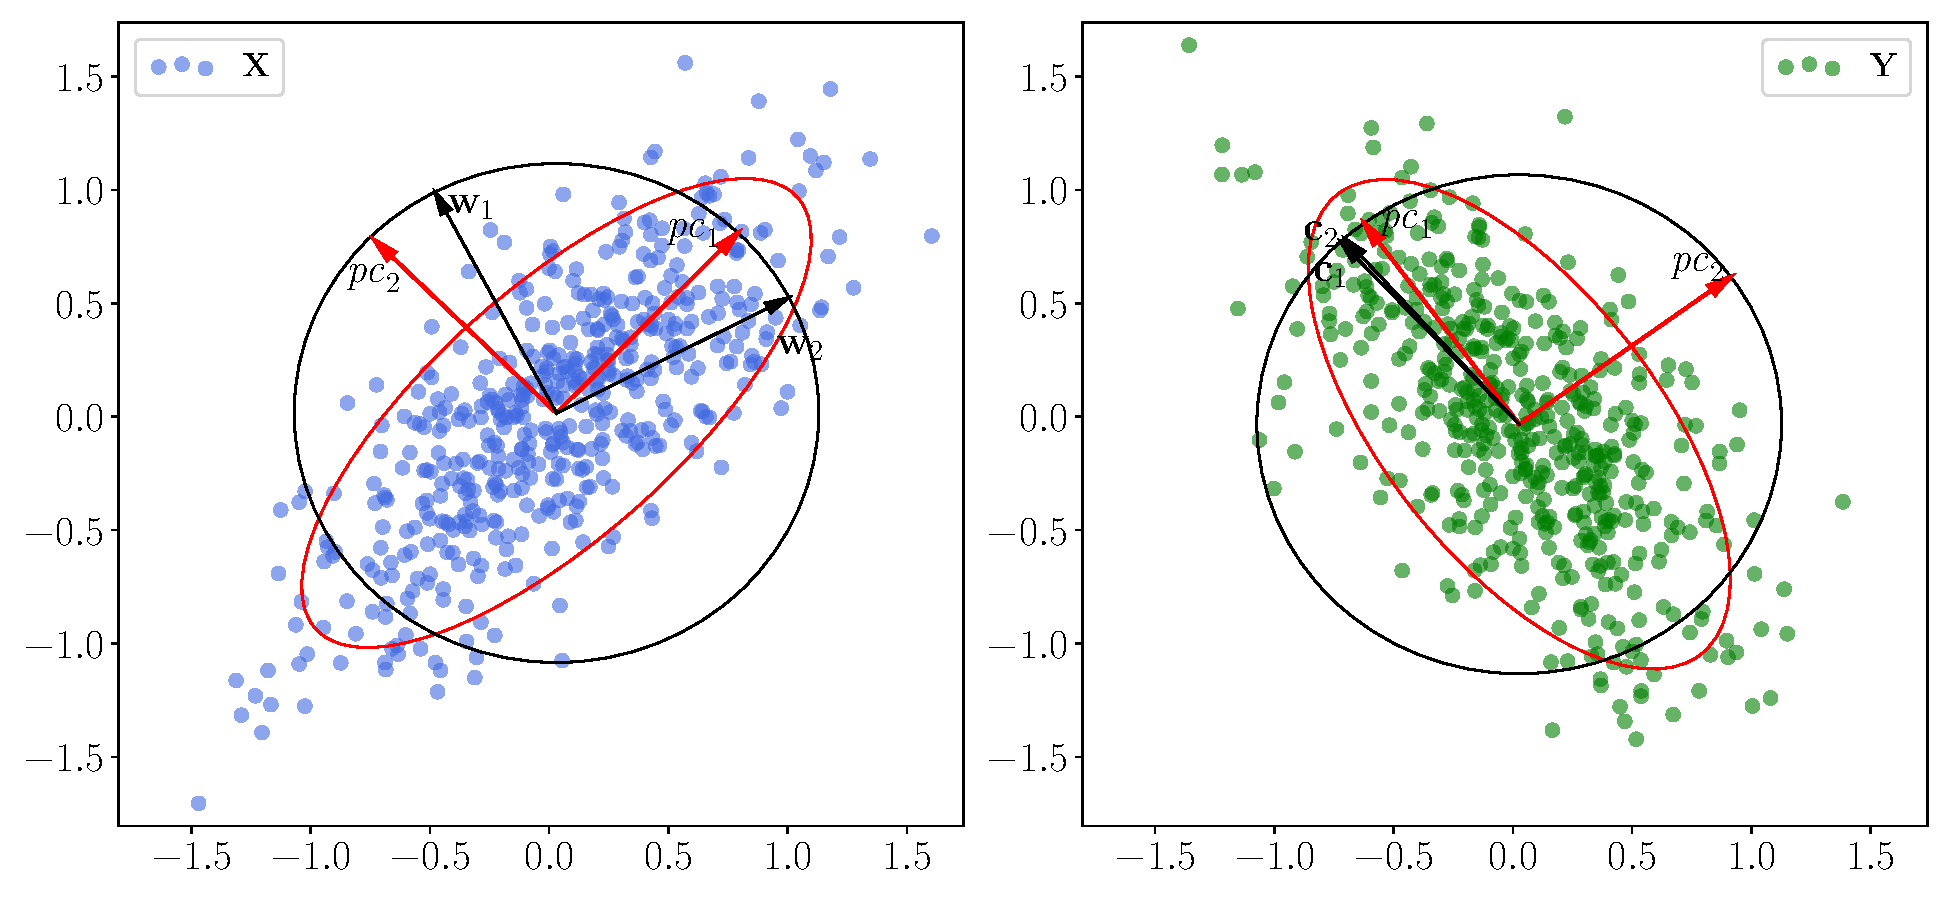
\includegraphics[width=\linewidth]{figs/ch1/pls_toy_example}
	\caption{Модельный пример работы алгоритмов PCA и PLS}
	\label{ch1:fig:pls_toy_example}
\end{figure}

При снижении размерности пространств до одного признака алгоритм PCA выберет первую главную компоненту $pc_1$, отбросив компоненту $pc_2$, так как первая компонента объясняет большую части дисперсии исходной матрицы $\bX$. 
При этом матрица $\bY$ не зависит от $pc_1$. 
Тем самым финальная модель окажется не оптимальной.
Алгоритм PLS позволяет побороться с данной проблемой.

\subsection{CCA}

Канонический корреляционный анализ (canonical correlation analysis, CCA) широко применяется для поиска взаимосвязи между двумя наборами переменных~\cite{hotelling1992relations,anderson1962introduction}. 
Оптимизационная задача CCA похожа на оптимизационную задачу PLS~\eqref{ch1:eq:pls_max_cov} с той лишь разницей, что вместо максимизации ковариации CCA максимизирует корреляцию:
\begin{equation}
	\max_{\|\bp\|_{2}=\|\bq\|_{2}=1}[ corr(\bX \bp, \bY \bq)^{2}] = \max_{\bp, \bq} \frac{\bp^{\T} \bX^{\T} \bY \bq}{\sqrt{\bp^{\T} \bX^{\T}  \bX \bp} \sqrt{\bq^{\T} \bY^{\T}  \bY\bq}}.
	\label{ch1:eq:cca_max_corr}
\end{equation}

Задача~\eqref{ch1:eq:cca_max_corr} может быть также решена с помощью алгоритма~\ref{ch1:pls_pseudocode} с модификацией в шаге (11): $\bq_k := \bY_k^{\T}\bu_k/(\bu_k^{\T}\bu_k)$.
На Рис.~\ref{ch1:fig:cca_toy_example} показан результат работы алгоритма. Основное различие состоит в том, что вектора $\bc_1$ и $\bc_2$ в данном случае становятся ортогональными.

\begin{figure}[h]
	\centering
	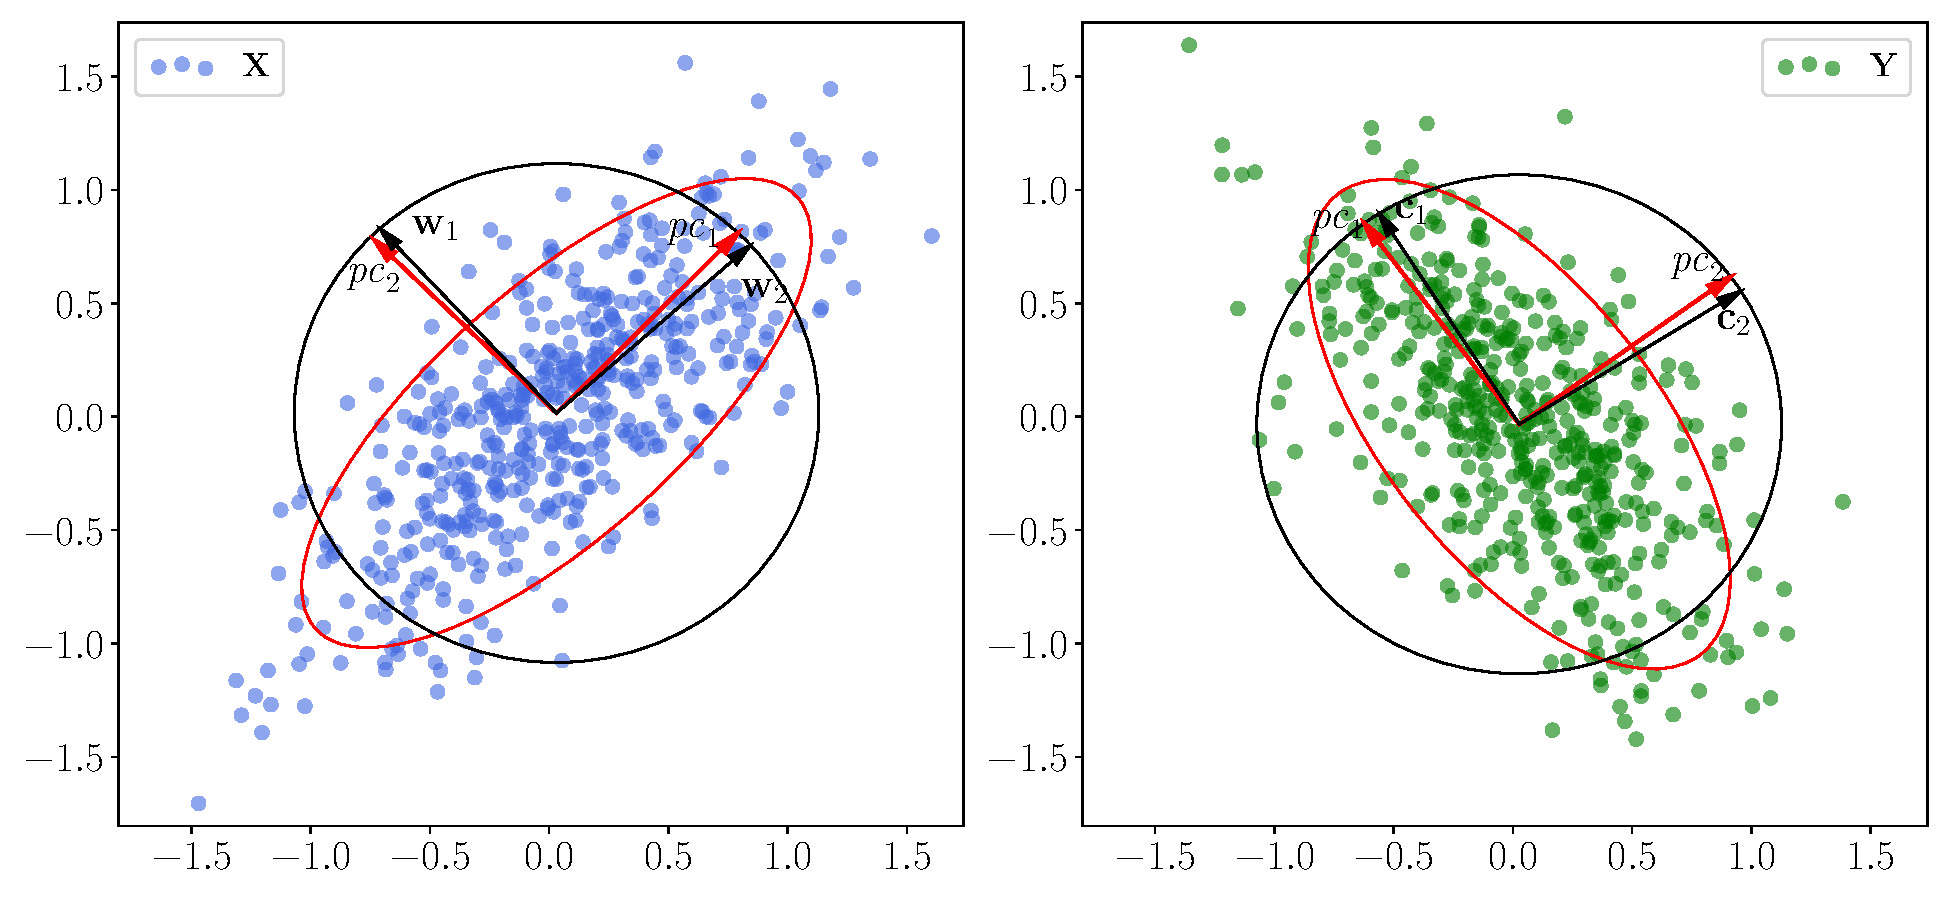
\includegraphics[width=\linewidth]{figs/ch1/cca_toy_example}
	\caption{Модельный пример работы алгоритмов PCA и CCA}
	\label{ch1:fig:cca_toy_example}
\end{figure}

В Таблице~\ref{ch1:tbl:toy_example_results} приведены значения квадратичной ошибки $\mathcal{L}(\bTheta, \bX, \bY)$ для алгоритмов линейной регрессии, PCA и PLS.

Нелинейный ядерный CCA~\cite{akaho2006kernel,melzer2001nonlinear,bach2002kernel,hardoon2004canonical} является обобщением базового метода. 
CCA и ядерный CCA широко используются для задач обучения без учителя~\cite{hardoon2007unsupervised,vinokourov2003inferring}. 
Метод имеет область применения от анализа хемометрических~\cite{montanarella1995chemometric} и биологических~\cite{vert2003graph} данных до обработки естественного языка~\cite{haghighi2008learning,dhillon2011multi}, аудиосигналов~\cite{choukri1986adaptation,rudzicz2010adaptive} и компьютерного зрения~\cite{kim2007tensor}.

В работе~\cite{andrew2013deep} был впервые предложено обобщение алгоритма CCA, работающего с нейросетями. 
Предложенный алгоритм DeepCCA максимизирует корреляцию между представлениями, полученными на выходе нейросети. 
Принцип работы алгоритма изображен на рисунке~\ref{ch1:fig:deepcca_schema}.
В статье~\cite{wang2015deep} приведен обширный обзор модификаций нейросетевого CCA для работы с многовидовыми данными.
Главным недостатком нейросетевого CCA является вычислительная сложность. 
В работе~\cite{chang2018scalable} предложена релаксация исходного лосса, которая способна масштабироваться под работу с большими глубокими моделями.

\begin{figure}[h]
	\centering
	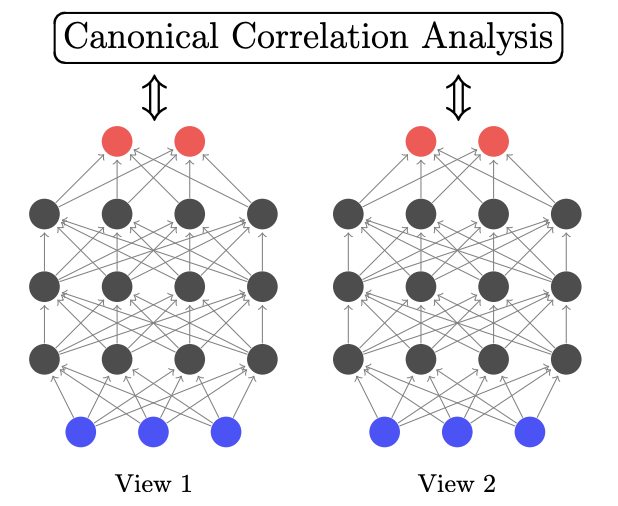
\includegraphics[width=0.5\linewidth]{figs/ch1/deepcca_schema}
	\caption{Схематичный пример работы алгоритма DeepCCA из работы~\cite{andrew2013deep}}
	\label{ch1:fig:deepcca_schema}
\end{figure}

\begin{table}[]
	\centering
	\begin{tabular}{|c|c|c|c|}
		\hline
		\textbf{Линейная регрессия} & \textbf{PCA}   & \textbf{PLS}  &  \textbf{CCA}  \\ \hline
		0.01 &  0.24   &  0.13 &  0.13 \\ \hline
	\end{tabular}
	\caption{Средняя квадратичная ошибка на модельном примере для алгоритмов линейной регрессии, PCA, PLS, CCA}
	\label{ch1:tbl:toy_example_results}
\end{table} 


\subsection{High order PLS/CCA}

\subsection{Многовидовые данные}

На практике возникают задачи, где каждый объект имеет несколько представлений. 
Каждое представление может представлять одну из модальностей. 
Примерами таких представлений и модальностей могут быть выровненные аудио и видео~\cite{kidron2005pixels,chaudhuri2009multi}, аудио и артикуляция~\cite{arora2012kernel}, изображение и текстовая аннотация~\cite{hardoon2004canonical,socher2010connecting,hodosh2013framing}, параллельный корпус текстов~\cite{vinokourov2003inferring,haghighi2008learning,ap2014autoencoder,faruqui2014improving}.

В случае если для каждого объекта имеется более двух представлений, то для построения скрытого пространства для каждого из них применяются два класса подходов. 
Первый подход состоит в построении скрытого пространства для каждой пары представлений объекта~\cite{masci2013multimodal,rajendran2015bridge}. 
Второй же подход состоит в построении общего единого скрытого пространства для всех представлений~\cite{kumar2011co,sharma2012generalized}.

\hrulefill

Преобразование PCA задается ортогональной матрицей $\bP$. Функция кодирования объектов имеет вид $\varphi_e(\bx) = \bP^{\T}\bx$. Функция декодирования объектов имеет вид $\varphi_d(\bt) = \bP\bt$. 

Функция кодирования и декодирования ответов являются тождественными преобразованиями $\psi_e(\by) =  \by = \bu = \psi_d(\bu)$. Преобразование $h$ является линейным.

Метод PCA не согласует объекты $\bx$ и ответы $\by$.


\hrulefill

Для PLS  функции кодирования имеют вид:
\begin{equation}
	\varphi_e(\bx) = \bW_{\bx}^{\T}\bx , \;\;
	\psi_e(\bY) = \bW_{\by}^{\T}\by ,
\end{equation} 
где матрицы весов $\bW_{\bx} \in \mathbb{R}^{m \times p}, \bW_{\by} \in \mathbb{R}^{k \times p}$. Столбцы матриц весов $\bw_{\bx}^{*}$ и $\bw_{\by}^{*}$ 
находятся путем максимизации функции согласования $g(\bX \bw_{\bx}, \bY \bw_{\by}) = cov (\bX \bw_{\bx}, \bY \bw_{\by})^{2}$:
\begin{equation}
	(\bw_{\bx}^{*}, \bw_{\by}^{*}) = \argmax_{\|\bw_{\by}\|_{2}=\|\bw_{\by}\|_{2}=1}[ cov(\bX \bw_{\bx}, \bY \bw_{\by})^{2}]
	\label{eq:PLSpr3}
\end{equation}
где $cov(\bX \bw_{\bx}, \bY \bw_{\by})$~-- выборочная ковариация между векторами.

Функции декодирования принимают следующий вид:
\begin{equation}
	\varphi_d(\bt) = \bP\bt, \;\;
	\psi_d(\bu) = \bQ\bu.
\end{equation} 

\hrulefill

Канонический корреляционный анализ (canonical correlation analysis, CCA) находит два набора базисных векторов $\{\bw_{\bx_i}\}_{i=1}^{p}, \; \bw_{\bx} \in \mathbb{R}^{m}$ и $\{\bw_{\by_i}\}_{i=1}^{p}, \; \bw_{\by} \in \mathbb{R}^{k}$, один для $\bX$ и другой для $\bY$, так что коэффициент корреляция между проекциями переменных на эти базисные векторы была максимальной. Функция согласования для CCA
\begin{equation}
	g(\bX \bw_{\bx}, \bY \bw_{\by}) = corr(\bX \bw_{\bx}, \bY \bw_{\by}),
\end{equation} 
где $corr(\bX \bw_{\bx}, \bY \bw_{\by})$~-- коэффициент корреляции между векторами.

Таким образом, функии кодирования
\begin{equation}
	\varphi_e(\bx) = \bW_{\bx}^{\T}\bx , \;\;
	\psi_e(\bY) = \bW_{\by}^{\T}\by ,
\end{equation}

где первые столбцы матриц весов находится, как вектора максимизирующие функцию согласования $g$. Далее ищутся вектора, максимизирующие $g$, но с ограничением, что они не коррелируют с первой парой векторов. Процедура продолжается до тех пор, пока количество векторов не станет равным $p$. 
 
\hrulefill
 
Для постановки задачи декодирования введём предположения о структурах пространств $\bbX$ и $\bbY$.
\begin{assumption}
	Рассмотрим случай, когда пространства $\bbX$ и $\bbY$ избыточны. Это означает, что объекты $\bx$ и $\by$ живут на некоторых многообразиях низкой размерности. В простейшем случае такие многообразия могут являться линейными подпространствами.
\end{assumption}

\begin{definition}
	Назовём пространство $\bbT \subset \bbR^l$ \textit{скрытым пространством} для пространства $\bbX \in \bbR^n$ ($l \leq n$), если существуют функция $\varphi_e: \bbX \to \bbT$ и функция $\varphi_d: \bbT  \to \bbX$ такие что
	\[
		\forall \bx \in \bbX \quad \exists \bt \in \bbT: \varphi_d (\varphi_e(\bx)) = \varphi_d(\bt) = \bx.
	\]
	Функцию $\varphi_e(\bx)$ будем называть \textit{функцией кодирования} объекта $\bx$, функцию $\varphi_d(\bt)$ будем называть \textit{функцией декодирования}. 
	
	
	Аналогично введём определение \textit{скрытого пространства}~$\bbU \subset \bbR^s$ для целевого пространства $\bbY$, \textit{функции кодирования} $\psi_e: \bbY \to \bbU$ и \textit{декодирования} $\psi_d: \bbU  \to \bbY$
	\[
	\forall \by \in \bbY \quad  \exists \bu \in \bbU: \psi_d (\psi_e(\by)) = \psi_d(\bu) = \by.
	\]
\end{definition}

\begin{definition}
	Будем считать, что пространство $\bbT \subset \bbR^l$ задаёт \textit{внутреннюю структуру} пространства $\bbX \in \bbR^n$, если пространство $\bbT$ является скрытым для пространства $\bbX$.
\end{definition}

\begin{definition}
	Между пространствами $\bbX$ и $\bbY$ существует \textit{согласующее отображение}, если существуют пространства $\bbT$ и $\bbU$, задающие внутренние структуры для пространств $\bbX$ и $\bbY$ соответственно, и существует \textit{функция согласования} $g: \bbT \rightarrow \bbU$, такая что
	\[
	 \forall \bu \in \bbU \quad \exists \bt:  \bu = g(\bt).
	\]
\end{definition}

\begin{assumption}
	Предположим, что в задаче предсказания~\eqref{ch1:eq:loss_min} пространства $\bbT$ и $\bbU$ задают внутреннюю структуру пространств $\bbX$ и $\bbY$. 
	Предположим также, что для данных скрытых пространств $\bbT$ и $\bbU$ существует функция согласования~$g: \bbT \rightarrow \bbU$. Тогда выполнено
	\[
	\forall \by \in \bbY \quad \exists \bx \in \bbX: \by = \psi_d(\bu) = \psi_d(g(\bt)) = \psi_d(g(\phi_e(\bx))). 
	\]
	
	Тогда общая схема задачи декодирования принимает вид следующей коммутативной диаграммы:
	\begin{equation}
	\begin{tikzpicture}
	\matrix (m) [matrix of math nodes,row sep=3em,column sep=4em,minimum width=2em]
	{
		\bbX \subset \bbR^n & \bbY \subset \bbR^r \\
		\bbT \subset \bbR^l & \bbU \subset \bbR^s \\};
	\path[-stealth]
	(m-1-1) edge node [above] {$f$} (m-1-2)
	(m-2-1) edge [bend right=10] node [right] {$\varphi_d$} (m-1-1)
	(m-2-2) edge [bend left=10] node [left] {$\psi_d$} (m-1-2)
	(m-1-1) edge [bend right=10] node [left] {$\varphi_e$} (m-2-1)
	(m-1-2) edge [bend left=10] node [right] {$\psi_e$} (m-2-2)
	(m-2-1) edge node [above] {$h$} (m-2-2);
	\end{tikzpicture}
	\label{ch1:eq:decoding_scheme}
	\end{equation}
\end{assumption}

\begin{definition}
	Согласно схеме~\eqref{ch1:eq:decoding_scheme}, определим модель декодирования $f: \bbX \rightarrow \bbY$ как суперпозицию
	 \begin{equation}
	 	f = \psi_d \circ g \circ \varphi_e.
	 	\label{ch1:eq:def_decoding_function}
	 \end{equation}
\end{definition}

Рассмотрим случай квадратичной функции потерь:
\[
\cL(f, \bX, \bY) = \sum_{i=1}^m \| \by_i - f(\bx_i) \|^2.
\]

\begin{statement}
	\label{ch1:st:decod_lip}
	Пусть функция декодирования $\psi_d$ модели декодирования~$f$~\eqref{ch1:eq:def_decoding_function} Липшицева с константой $L$. Тогда 
	\[
		\cL(f, \bX, \bY) \leq L \cdot \cL(g, \bT, \bU).
	\]
\end{statement}

\begin{proof}
	\begin{multline*}
		\cL(f, \bX, \bY) = \sum_{i=1}^m \| \psi_d (g (\phi_e(\bx_i))) - \by_i \|^2  = \sum_{i=1}^m \| \psi_d (g (\bt_i)) - \psi_d (\bu_i) \|^2 \\\leq L \sum_{i=1}^m \| g (\bt_i) - \bu_i \|^2 = L \cdot \cL(g, \bT, \bU).
	\end{multline*}
\end{proof}
\begin{theorem}
	Рассмотрим две модели:
	\begin{enumerate}
		\item Первая модель $f_1$ доставляет минимум ошибке $\cL(f, \bX, \bY)$
		\[
		f_1 = \argmin_f \cL(f, \bX, \bY).
		\]
		При этом $\bY = f_1(\bX) + \bE_1$, где $\bE_1 \in \bbR^{m \times r}$~--- матрица ошибок модели $f_1$.
		
		\item Вторая модель $f_2$~--- модель декодирования~\eqref{ch1:eq:def_decoding_function} c Липшецевой функцией декодирования $\psi_d$ с константой $L$ и функцией согласования, удовлетворяющей условию
		\[
			g = \argmin_g \cL(g, \bT, \bU).
		\]
		При этом $\bU = g(\bT) + \bE_2$, где $\bE_2 \in \bbR^{m \times s}$~--- матрица ошибок функции согласования $g$.
	\end{enumerate}
	Пусть для константы Липшица $L$ функции декодирования $\psi_d$ выполнено следующее условие
	\begin{equation}
		L \leq \frac{\|\bE_1\|_F^2}{\|\bE_2\|_F^2}.
		\label{ch1:eq:lip_ineq}
	\end{equation}
	Тогда функция ошибки $\cL(f_2, \bX, \bY)$ модели $f_2$ не превосходит функции ошибки $\cL(f_1, \bX, \bY)$ модели $f_1$.
\end{theorem}

\begin{proof}
	\[
		\mathcal{L} (f_1, \bX, \bY) = \sum_{i=1}^m \| \mathbf{f}_1(\bx_i) - \by_i\|^2 = \| \bE_1 \|_F^2.
	\]
	\[
	\mathcal{L} (g, \bT, \bU) = \sum_{i=1}^m \| \mathbf{g}(\bt_i) - \bu_i\|^2 = \| \bE_2 \|_F^2.
	\]
	Воспользуемся утверждением~\ref{ch1:st:decod_lip} и условием~\eqref{ch1:eq:lip_ineq}
	\[
		\mathcal{L} (f_2, \bX, \bY) \leq L \cdot \cL(g, \bT, \bU) = L \| \bE_2 \|_F^2 \leq \| \bE_1 \|_F^2 = \cL(f_1, \bX, \bY).
	\]
\end{proof}

\hrulefill

\begin{definition}
	Функция $g: \bbR^l \times \bbR^l \to \bbR$, связывающая два низкоразмерных латентных представления, назовём \textit{функцией согласования}.
\end{definition}
где $\varphi_e: \bbR^m \to \bbR^l$~--  функция кодирования объектов; $\psi_e: \bbR^r \to \bbR^l$~--  функция кодирования ответов; $\varphi_d: \bbR^l \to \bbR^n$~--  функция декодирования объектов; $\psi_d: \bbR^l \to \bbR^r$~--  функция декодирования ответов; $\bT = [\varphi_e(\bx_1), \cdots, \varphi_e(\bx_m)]^{\T}  \in \bbR^{m\times l}$ и $\bU =[\psi_e(\by_1), \cdots, \psi_e(\by_m)]^{\T} \in \bbR^{m\times l}$~-- матрицы представлений данных в латентном пространстве низкой размерности; $g: \bbR^l \times \bbR^l \to \bbR$~-- функция согласования.

Оптимальные параметры $\bW_{\varphi_e}^{*}, \bW_{\psi_e}^{*}$ для функций кодирования $\varphi_e$  и $\psi_e$ находятся из следующей задачи параметрической оптимизации:
\begin{equation}
(\bW_{\varphi_e}^{*}, \bW_{\psi_e}^{*}) = \argmax_{(\bW_{\varphi_e}, \bW_{\psi_e})} [g(\varphi_e(\bX; \bW_{\varphi_e}), \psi_e(\bY; \bW_{\psi_e})))].
\label{ch1:eq:alignment_argmax}
\end{equation}

{\color{red} Изменить} Так как параметры функции кодирования подбирались из условия максимизации функции согласования~\eqref{ch1:eq:alignment_argmax} , то после перехода в латентное пространство между $\mathbf{T}$ и $\mathbf{U}$ существует зависимость
\begin{equation}
\bU = h(\bT) +  \boldsymbol{\eta},
\label{ch1:eq:alignment_regression}
\end{equation}
где $h: \mathbb{R}^{n \times p} \to \mathbb{R}^{n \times p}$~-- функция регрессионной зависимости,  $\boldsymbol{\eta}$~-- матрица регрессивных ошибок.

Оптимальная $h$ находится минимизацией функции ошибки. Используем квадратичную функцию ошибки потерь $\mathcal{L}$ на $\bT$ и $\bU$:
\begin{equation}
\mathcal{L}(h | {\bT}, {\bU}) = {\left\| \underset{n \times p}{\bU}  - h(\underset{m \times p}{\bT}) \right\| }_2^2 \rightarrow\min_{h}.
\label{ch1:eq:alignment_regression_loss}
\end{equation}

Финальная прогностическая модель имеет вид:
$\widehat{\by} = \psi_d(h(\varphi_e(\bx)))$, то есть

\begin{equation}
f = \psi_d \circ h \circ \varphi_e
\label{eq:f}
\end{equation}

\begin{figure}[!ht]
	\centering
	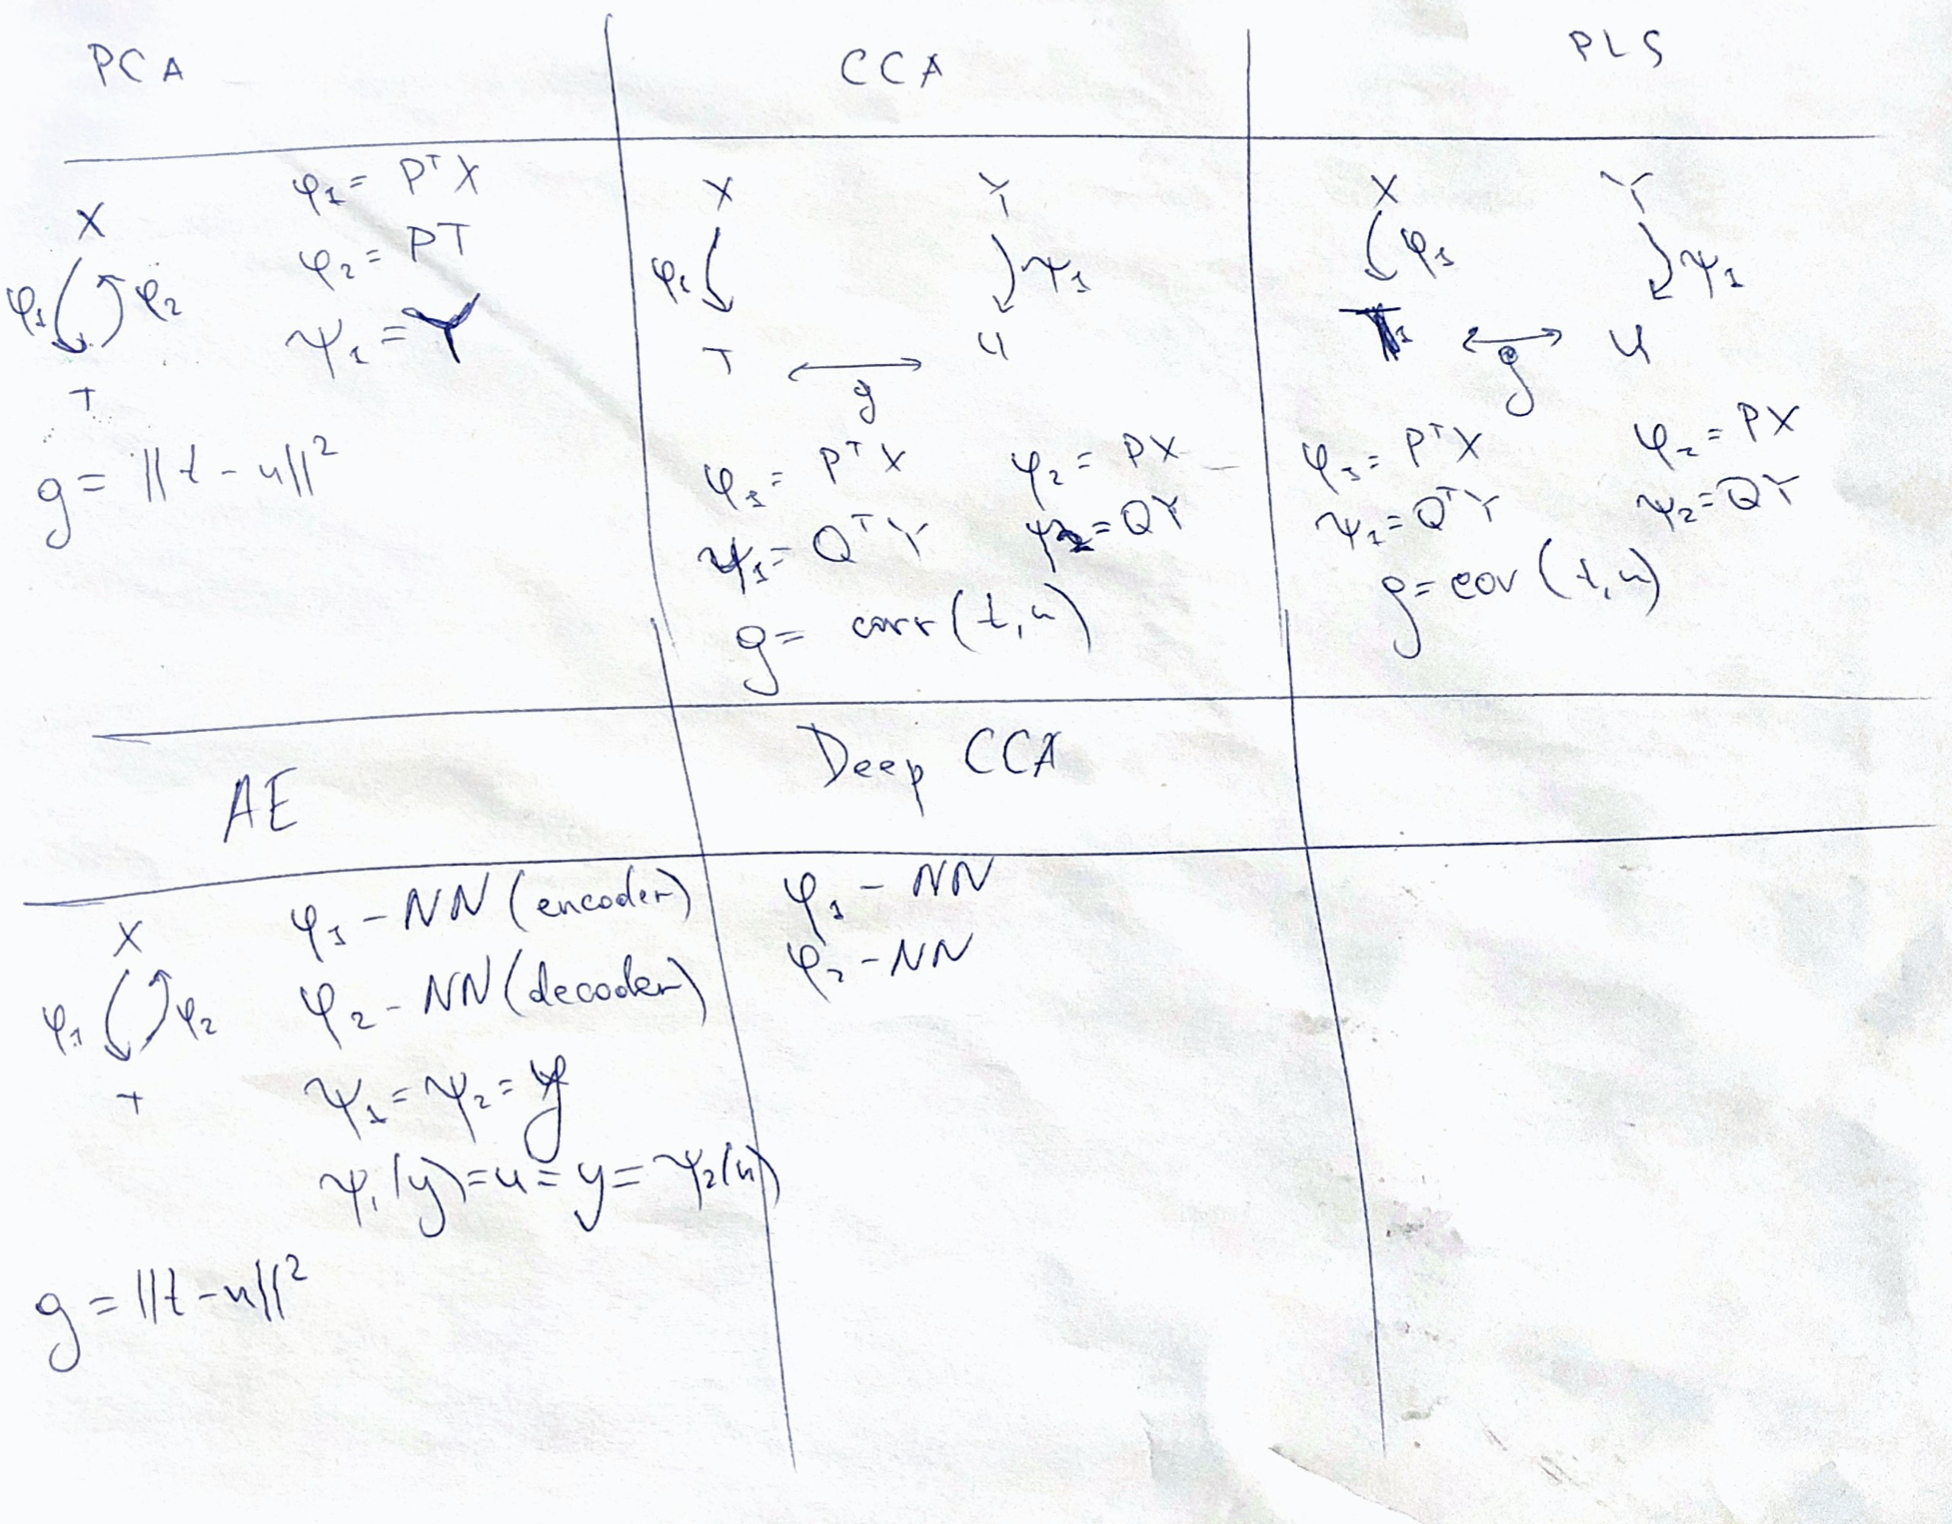
\includegraphics[width=\linewidth]{figs/ch1/Examples}
	\caption{Примеры алгоритмов, работающих по схеме \ref{ch1:eq:decoding_scheme}}
	\label{ch1:fig:PLSFigure}
\end{figure}

\subsection{Deep CCA}

Deep CCA~-- нелинейной модификация CCA. DCCA преобразует исходные данные с помощью многослойной нейронной сети таким образом, что результирующее представление становится согласованным. Предполагается, что есть $d$ слоев нейроной сети. 

Выходом первого слоя для экземпляра $\bx$ будет $\mathbf{h}_1 = s(\bW^{1}_{\bx}\bx + \bb^{1}_{\bx}) \in \mathbb{R}^{c_1}$, где $\bW_{\bx}^{1} \in \mathbb{R}^{c_1 \times m}$~-- матрица весов, $\bb_{x}^{1} \in \mathbb{R}^{c_1}$~-- вектор смещения, $s: \mathbb{R} \to \mathbb{R}$~-- нелинейная функция, которая действует покомпонентно. Далее выход первого слоя используется для вычисления выхода второго слоя $\mathbf{h}_{2} = s(\bW^{2}_{\bx}\mathbf{h}_{1} + \bb^{2}_{\bx}) \in \mathbb{R}^{c_2}$ и так далее до тех пор пока не будет найдено конечное представление $\varphi_e(\bx) = s(\bW^{d}_{\bx}\mathbf{h}_{d-1} + \bb^{d}_{\bx}) \in \mathbb{R}^{p}$. Аналогично находится представление для $\by$: $\psi_e(\by) = s(\bW^{d}_{\by}\mathbf{h}_{d-1} + \bb^{d}_{\by}) \in \mathbb{R}^{p}.$

Обозначим $\theta_{\bx}$, $\theta_{\by}$~-- параметры для функций кодирования, то есть матрицы весов и векторы смещений. Оптимальные параметры $\theta_{\bx}^{*}$, $\theta_{\by}^{*}$ находятся из задачи оптимизации:
\begin{equation}
(\theta_{\bx}^{*}, \theta_{\by}^{*}) = \argmax _{(\theta_{\bx}, \theta_{\by})} [g(\varphi_e(\bX; \theta_{\bx}), \psi_e(\bY; \theta_{2}))] = \argmax _{(\theta_{\bx}, \theta_{\by})} [corr(\varphi_e(\bX; \theta_{\bx}), \psi_e(\bY; \theta_{2}))].
\end{equation}

%%%%%%%%%%%%%%%%%%%%%%%%%%%%%%%%%%%%%%%%%%%%%%%%
\section{Вычислительный эксперимент}
%%%%%%%%%%%%%%%%%%%%%%%%%%%%%%%%%%%%%%%%%%%%%%%%

Временные ряды электроэнергии состоят из почасовых записей (52512 наблюдений). 
Строка матрицы~$\bX$~--– локальная история сигнала за одну неделю $n = 24 \times 7$. Строка матрицы~$\bY$~--- локальный прогноз потребления электроэнергии в следующие 24 часа $r = 24$. В этом случае матрицы~$\bX$ и~$\bY$ являются авторегрессионными матрицами.

Вычислительный эксперимент также проводился на данных электрокортикограмм (ECoG) из проекта NeuroTycho~\cite{shimoda2012decoding}.
Данные ECoG состоят из 32-канальных сигналов напряжения, снятых с головного мозга.
Цель состоит в предсказании по входному сигналу ECoG 3D позиции рук в последующие моменты времени.
Исходные сигналы напряжения преобразуются в пространственно-временное представление с помощью вейвлет-преобразования с материнским вейвлетом Морле.
Процедура извлечения признаков из исходных данных подробно описана в~\cite{chao2010long,eliseyev2016penalized}.
Описание исходного сигнала в каждый момент времени имеет размерность 32 (каналы) $\times $ 27 (частоты) = 864.
Каждый объект представляет собой локальный отрезок времени длительностью $\Delta t = 1s$. Временной шаг между объектами $\delta t = 0.05 s$.
Матрицы имеют размеры $\bX \in \bbR^{18900 \times 864}$ и $\bY \in \bbR^{18900 \times 3k}$, где $k$ - число отсчётов времени прогнозирования.
Данные разбиты на тренировочную и тестовую части в соотношении 0,67. 
Пример исходных сигналов мозга и соответствующей траектории руки показан на рисунке~\ref{ch2:fig:ecog_data}.

\begin{figure}
	\centering
	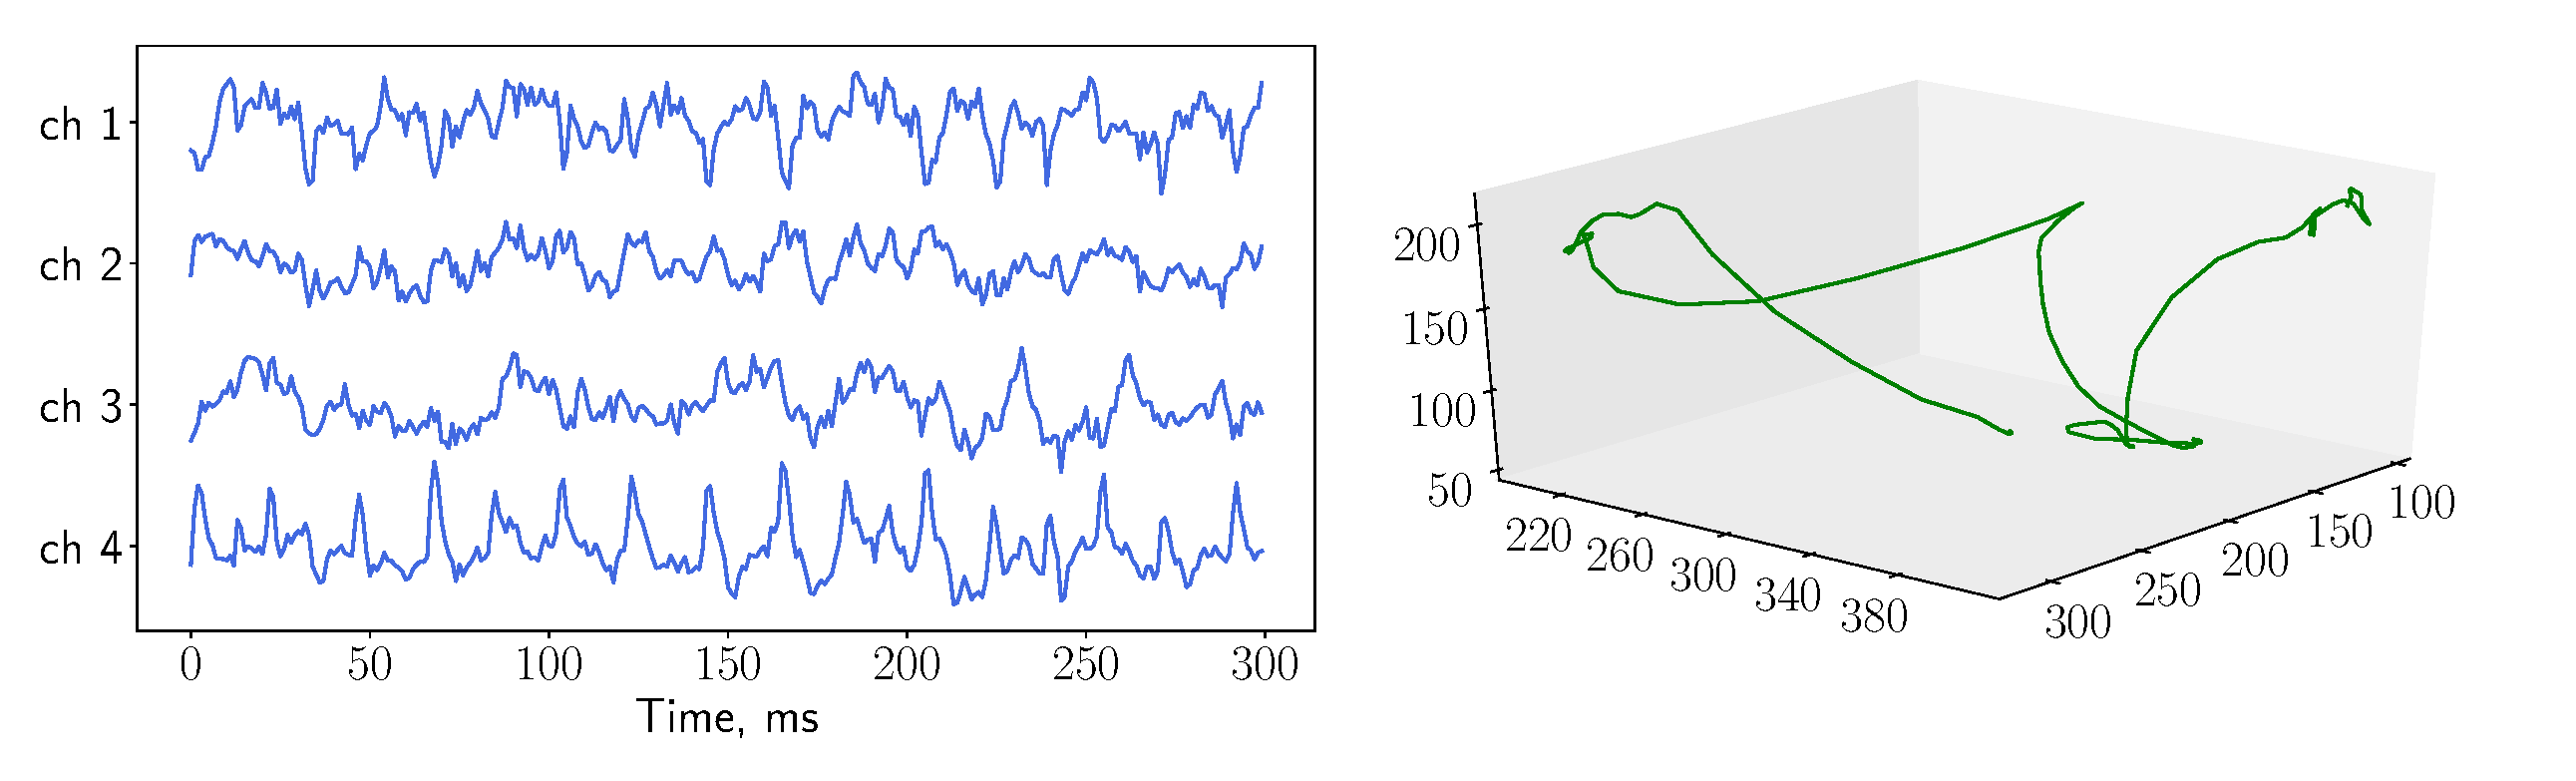
\includegraphics[width=\linewidth]{figs/ch2/ecog_data}
	\caption{Сигналы мозга (левый график) и 3D координаты руки (правый график)}
	\label{ch1:fig:ecog_data}
\end{figure}

Введём среднеквадратичную ошибку для некоторых матриц $\mathbf{A} = [a_{ij}]$ и $\mathbf{B} = [b_{ij}]$
\[
\text{MSE} (\mathbf{A}, \mathbf{B}) = \sum_{i,j} (a_{ij} - b_{ij})^2.
\]
Для оценивания качества аппроксимации вычисляется значение нормированной среднеквадратичной ошибки
\begin{equation}
\text{NMSE}(\bY,  \mathbf{\hat{Y}}) = \frac{\text{MSE} (\bY, \mathbf{\hat{Y}})}{\text{MSE} (\bY, \mathbf{\bar{Y}})},
\label{ch1:eq:nmse}
\end{equation}
где $\mathbf{\hat{Y}}$~--- прогноз модели, $\mathbf{\bar{Y}}$~--- константный прогноз средним значением по столбцам матрицы.

\subsection*{Данные потребления электроэнергии}

Для нахождения оптимальной размерности $l$ латентного пространства все данные потребления электроэнергии были разбиты на обучающую и валидационную части. 
Обучающая выборка состоит из $700$ объектов, валидационная из $370$. Зависимость нормированной квадратичной ошибки~\eqref{ch1:eq:nmse} от размерности $l$ латентного пространства представлена на Рис.~\ref{ch1:fig:energy_n_comp}. 
Сначала ошибка резко падает при увеличении размерности скрытого пространства, а затем стабилизируется.

\begin{figure}[ht]
	\centering
	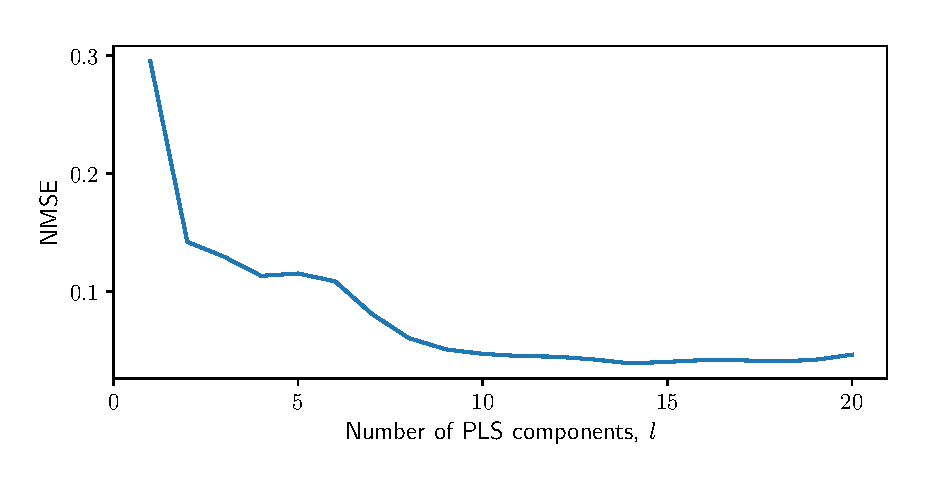
\includegraphics[width=0.75\linewidth]{figs/ch1/energy_n_comp}
	\caption{Прогноз потребления электроэнергии алгоритмом PLS при размерности латентного пространства $l$=14}
	\label{ch1:fig:energy_n_comp}
\end{figure}

Минимальная ошибка наблюдается при $l=14$. 
Построим прогноз потребления электроэнергии при данном $l$. 
Результат аппроксимации изображен на Рис.~\ref{ch1:fig:energy_prediction}. Алгоритм PLS восстановил авторегрессионную зависимость и обнаружил дневную сезонность.

\begin{figure}[ht]
	\centering
	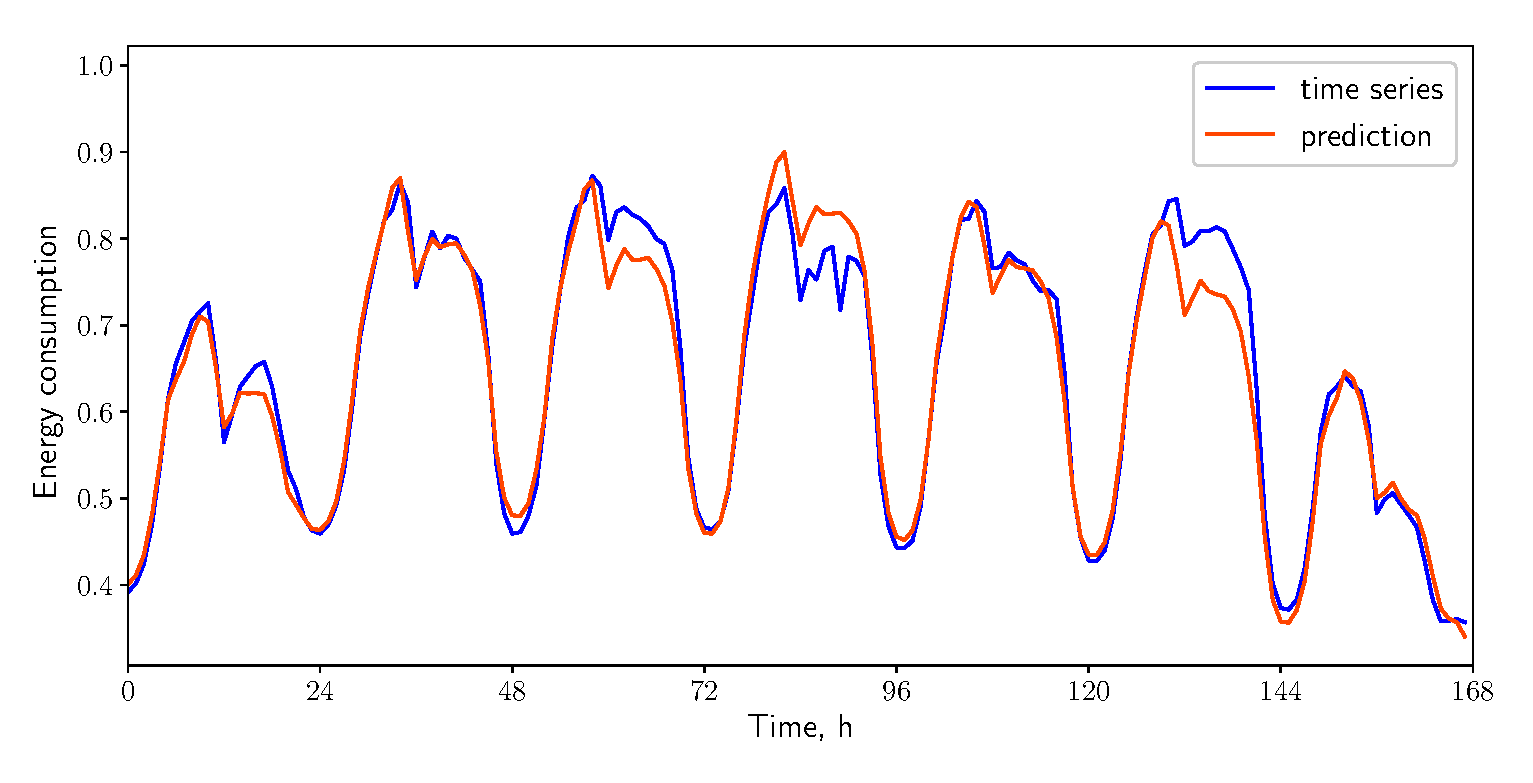
\includegraphics[width=0.95\textwidth]{figs/ch1/energy_prediction}
	\caption{Зависимость ошибки от размерности латентного пространства для данных потребления электроэнергии}
	\label{ch1:fig:energy_prediction}
\end{figure}

\subsection*{Данные электрокортикограммы}

На Рис.~\ref{ch1:fig:ecog_n_comp} представлена зависимость нормированной квадратичной ошибки~\eqref{ch1:eq:nmse} от размерности латентного пространства. Ошибка аппроксимации меняется незначительно при $l > 5$.
Таким образом совместное описание пространственно-временного спектрального представления объектов и пространственного положения руки может быть представлено вектором размерности $l \ll n$.
Зафиксируем $l = 5$. 
Пример аппроксимации положения руки изображен на Рис.~\ref{ch1:fig:ecog_prediction}. 
Сплошными линиями изображены истинные координаты руки по всем осям, пунктирными линиями показана аппроксимация методом PLS.
 
\begin{figure}[ht]
	\centering
	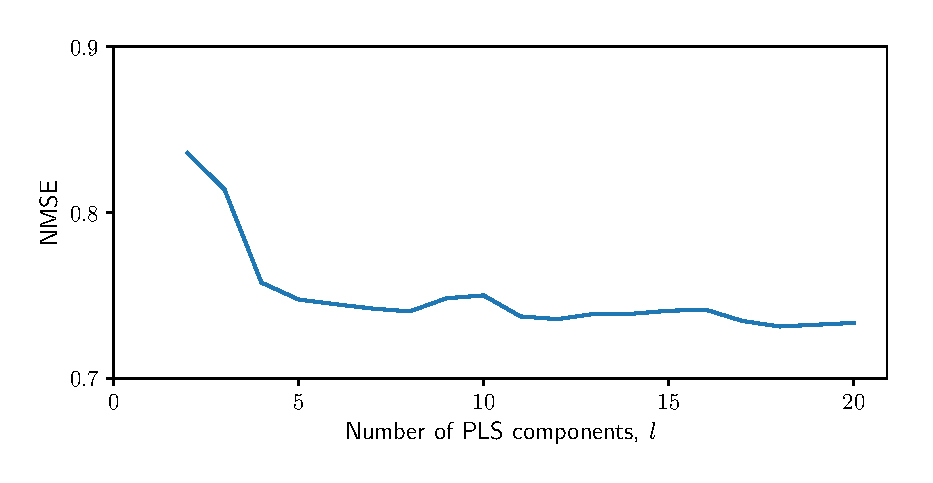
\includegraphics[width=0.75\linewidth]{figs/ch1/ecog_n_comp}	
	\caption{Зависимость ошибки от размерности латентного пространства для данных ECoG}
	\label{ch1:fig:ecog_n_comp}
\end{figure}

\begin{figure}[ht]
	\centering
	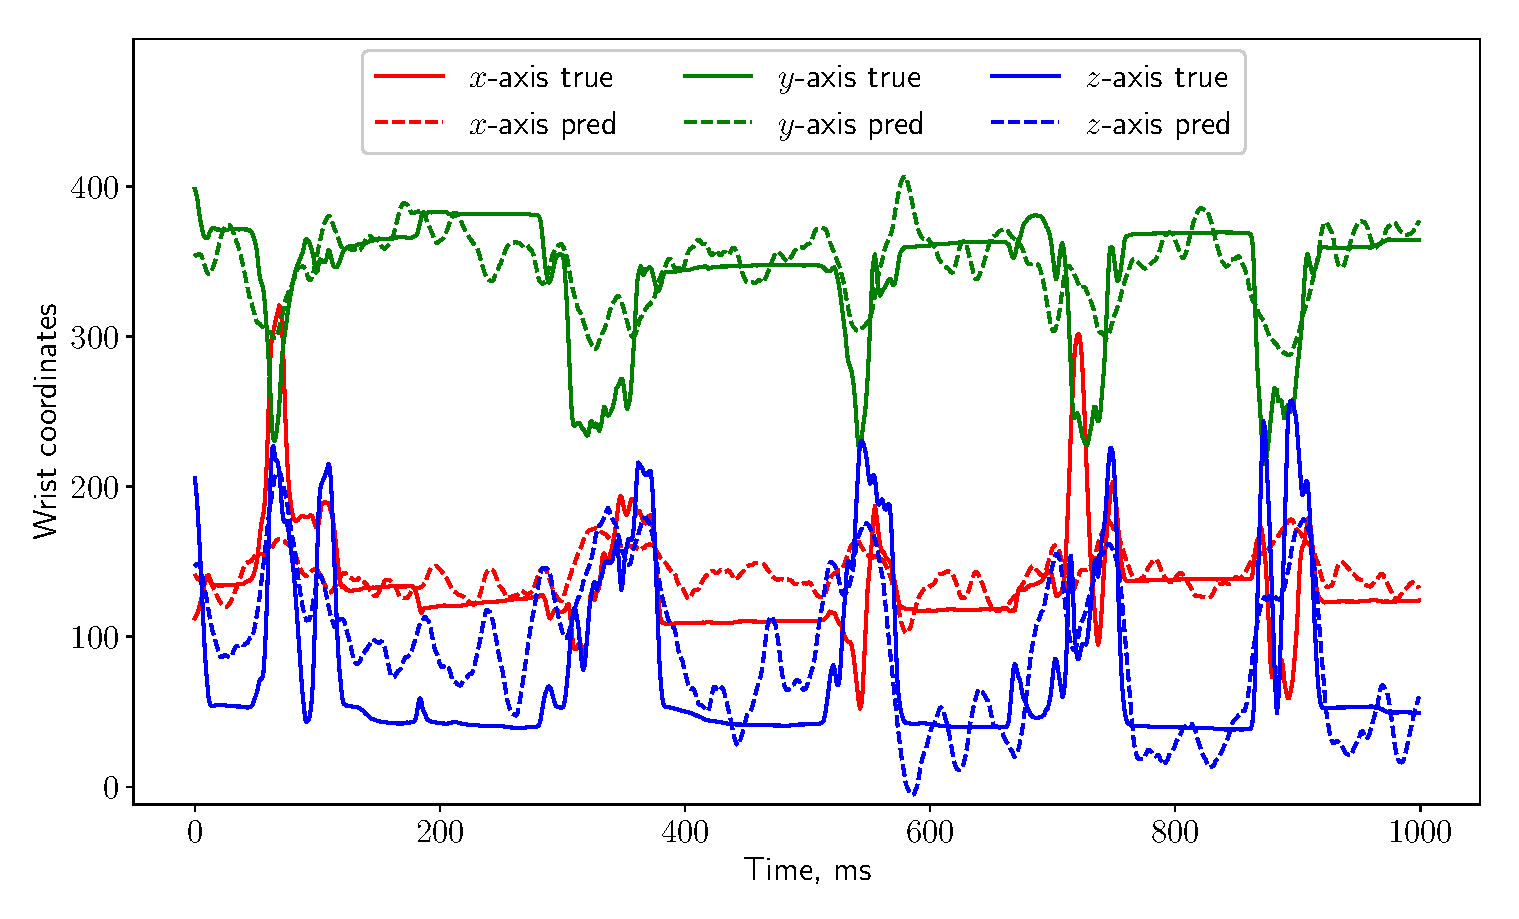
\includegraphics[width=\textwidth]{figs/ch1/ecog_prediction}
	\caption{Прогноз движения руки данных ECoG алгоритмом PLS при размерности латентного пространства $l=5$}
	\label{ch1:fig:ecog_prediction}
\end{figure}



\newpage{}
\chapter{Решение задачи декодирования в пространстве высокой размерности}
\label{chap:ch2}

\section{Формальная постановка задачи}

Для постановки задачи декодирования введём предположения о структурах пространств $\bbX$ и $\bbY$.
\begin{assumption}
	Рассмотрим случай, когда пространства $\bbX$ и $\bbY$ избыточны. Это означает, что объекты $\bx$ и $\by$ живут на некоторых многообразиях низкой размерности. В простейшем случае такие многообразия могут являться линейными подпространствами.
\end{assumption}

\begin{definition}
	Назовём пространство $\bbT \subset \bbR^l$ \textit{скрытым пространством} для пространства $\bbX \in \bbR^n$ ($l \leq n$), если существуют функция $\varphi_e: \bbX \to \bbT$ и функция $\varphi_d: \bbT  \to \bbX$ такие что
	\[
	\forall \bx \in \bbX \quad \exists \bt \in \bbT: \varphi_d (\varphi_e(\bx)) = \varphi_d(\bt) = \bx.
	\]
	Функцию $\varphi_e(\bx)$ будем называть \textit{функцией кодирования} объекта $\bx$, функцию $\varphi_d(\bt)$ будем называть \textit{функцией декодирования}. 
	
	
	Аналогично введём определение \textit{скрытого пространства}~$\bbU \subset \bbR^s$ для целевого пространства $\bbY$, \textit{функции кодирования} $\psi_e: \bbY \to \bbU$ и \textit{декодирования} $\psi_d: \bbU  \to \bbY$
	\[
	\forall \by \in \bbY \quad  \exists \bu \in \bbU: \psi_d (\psi_e(\by)) = \psi_d(\bu) = \by.
	\]
\end{definition}

\begin{definition}
	Будем считать, что пространство $\bbT \subset \bbR^l$ задаёт \textit{внутреннюю структуру} пространства $\bbX \in \bbR^n$, если пространство $\bbT$ является скрытым для пространства $\bbX$.
\end{definition}

\begin{definition}
	Между пространствами $\bbX$ и $\bbY$ существует \textit{согласующее отображение}, если существуют пространства $\bbT$ и $\bbU$, задающие внутренние структуры для пространств $\bbX$ и $\bbY$ соответственно, и существует \textit{функция согласования} $g: \bbT \rightarrow \bbU$, такая что
	\[
	\forall \bu \in \bbU \quad \exists \bt:  \bu = g(\bt).
	\]
\end{definition}

\begin{assumption}
	Предположим, что в задаче предсказания~\eqref{ch1:eq:loss_min} пространства $\bbT$ и $\bbU$ задают внутреннюю структуру пространств $\bbX$ и $\bbY$. 
	Предположим также, что для данных скрытых пространств $\bbT$ и $\bbU$ существует функция согласования~$g: \bbT \rightarrow \bbU$. Тогда выполнено
	\[
	\forall \by \in \bbY \quad \exists \bx \in \bbX: \by = \psi_d(\bu) = \psi_d(g(\bt)) = \psi_d(g(\phi_e(\bx))). 
	\]
	
	Тогда общая схема задачи декодирования принимает вид следующей коммутативной диаграммы:
	\begin{equation}
		\begin{tikzpicture}
			\matrix (m) [matrix of math nodes,row sep=3em,column sep=4em,minimum width=2em]
			{
				\bbX \subset \bbR^n & \bbY \subset \bbR^r \\
				\bbT \subset \bbR^l & \bbU \subset \bbR^s \\};
			\path[-stealth]
			(m-1-1) edge node [above] {$f$} (m-1-2)
			(m-2-1) edge [bend right=10] node [right] {$\varphi_d$} (m-1-1)
			(m-2-2) edge [bend left=10] node [left] {$\psi_d$} (m-1-2)
			(m-1-1) edge [bend right=10] node [left] {$\varphi_e$} (m-2-1)
			(m-1-2) edge [bend left=10] node [right] {$\psi_e$} (m-2-2)
			(m-2-1) edge node [above] {$h$} (m-2-2);
		\end{tikzpicture}
		\label{ch1:eq:decoding_scheme}
	\end{equation}
\end{assumption}

\begin{definition}
	Согласно схеме~\eqref{ch1:eq:decoding_scheme}, определим модель декодирования $f: \bbX \rightarrow \bbY$ как суперпозицию
	\begin{equation}
		f = \psi_d \circ g \circ \varphi_e.
		\label{ch1:eq:def_decoding_function}
	\end{equation}
\end{definition}

\section{Доказательство корректности работы алгоритмов PLS и CCA}

Псевдокод метода регрессии PLS приведен в алгоритме~\ref{ch1:pls_pseudocode}.
Алгоритм итеративно на каждом из $l$ шагов вычисляет по одному столбцу $\bt_k$, $\bu_k$, $\bp_k$, $\bq_k$ матриц $\bT$, $\bU$, $\bP$, $\bQ$ соответственно. 
После вычисления следующего набора векторов из матриц $\bX$, $\bY$ вычитаются очередные одноранговые аппроксимации. 
При этом предполагается, что исходные матрицы~$\bX$ и~$\bY$ нормированы (имеют нулевое среднее и единичное среднее отклонение).

\begin{algorithm}[h]
	\caption{Алгоритм PLS}
	\label{ch1:pls_pseudocode}
	\begin{algorithmic}[1]
		\REQUIRE $\bX, \bY, l$;
		\ENSURE $\bT, \bP, \bQ$;
		\STATE нормировать матрицы $\bX$ и $\bY$ по столбцам
		\STATE инициализировать $\bu_0$ (первый столбец матрицы $\bY$)
		\STATE $\bX_1 = \bX; \bY_1 = \bY$
		\FOR{$k=1,\dots, l$}
		\REPEAT
		\vspace{0.1cm}
		\STATE $\bw_k := \bX_k^{\T} \bu_{k-1} / (\bu_{k-1}^{\T} \bu_{k-1}); \quad \bw_k: = \frac{\bw_k}{\| \bw_k \|}$
		\vspace{0.1cm}
		\STATE $\bt_k := \bX_k \bw_k$
		\vspace{0.1cm}
		\STATE $\bc_k := \bY_k^{\T} \bt_k / (\bt_k^{\T} \bt_k); \quad \bc_k: = \frac{\bc_k}{\| \bc_k \|}$
		\vspace{0.1cm}
		\STATE $\bu_k := \bY_k \bc_k$
		\UNTIL{$\bt_k$ не стабилизируется}
		\vspace{0.1cm}
		\STATE $\bp_k:= \bX_k^{\T}\bt_k/(\bt_k^{\T}\bt_k),\ 
		\bq_k := \bY_k^{\T}\bt_k/(\bt_k^{\T}\bt_k)$
		\vspace{0.2cm}
		\STATE $\bX_{k+1} :=  \bX_k - \bt_k \bp_k^{\T}$
		\vspace{0.2cm}
		\STATE $\bY_{k + 1} :=  \bY_k - \bt_k \bq_k^{\T}$ 
		\ENDFOR
	\end{algorithmic}
\end{algorithm}

Вектора $\bt_k$ и $\bu_k$ из внутреннего цикла алгоритма~\ref{ch1:pls_pseudocode}
содержат информацию о матрице объектов $\bX$ и матрице ответов $\bY$ соответственно. 
Блоки из шагов (6)-(7) и шагов (8)-(9)~--- аналоги алгоритма PCA для матриц $\bX$ и $\bY$~\cite{geladi1988pls}. 
Последовательное выполнение блоков позволяет учесть взаимную связь между матрицами $\bX$ и $\bY$.

Теоретическое обоснование алгоритма PLS следует из следующих утверждений.
\begin{statement}
	Максимизации ковариации между векторами $\bt_k$ и $\bu_k$ сохраняет дисперсию матриц~$\bX$ и~$\bY$ и учитывает их линейную зависимость.
\end{statement}
\begin{proof}
	Утверждение следует из равенства
	\[
	\text{cov} (\bt_k, \bu_k) = \text{corr} (\bt_k, \bu_k) \cdot \sqrt{\text{var}(\bt_k)} \cdot \sqrt{\text{var}(\bu_k)}.
	\]
	Максимизация дисперсий векторов $\bt_k$ и $\bu_k$ отвечает за сохранение информации об исходных матрицах, 
	корреляция между векторами отвечает взаимосвязи между $\bX$ и~$\bY$. 
\end{proof}

Во внутреннем цикле алгоритма вычисляются нормированные вектора весов $\bw_k$ и $\bc_k$. 
Из данных векторов строятся матрицы весов $\bW$ и $\bC$ соответственно.

\begin{statement}
	В результате выполнения внутреннего цикла вектора $\bw_k$ и $\bc_k$ будут собственными векторами матриц $\bX_k^{\T} \bY_k \bY_k^{\T} \bX_k$ и $\bY_k^{\T} \bX_k \bX_k^{\T} \bY_k$, соответствующими максимальным собственным значениям.
	
	\begin{equation*}
		\bw_k \varpropto \bX_k^{\T} \bu_{k-1} \varpropto \bX_k^{\T} \bY_k \bc_{k-1} \varpropto \bX_k^{\T} \bY_k \bY_k^{\T} \bt_{k-1} \varpropto \bX_k^{\T} \bY_k \bY_k^{\T} \bX_k \bw_{k-1},
	\end{equation*}
	\begin{equation*}
		\bc_k \varpropto \bY_k^{\T} \bt_k \varpropto \bY_k^{\T} \bX_k \bw_k \varpropto \bY_k^{\T} \bX_k \bX_k^{\T} \bu_{k-1} \varpropto \bY_k^{\T} \bX_k \bX_k^{\T} \bY_k \bc_{k-1},
	\end{equation*}
	где символ $\varpropto$ означает равенство с точностью до мультипликативной константы. 
	\label{st:eig}
\end{statement}
\begin{proof}
	Утверждение следует из того факта, что правила обновления векторов $\bw_k$, $\bc_k$ совпадают с итерацией алгоритма поиска максимального собственного значения. 
	Данный алгоритм основан на следующем факте.
	
	Если матрица $\mathbf{A}$ диагонализуема, $\bx$~--- некоторый вектор, то
	
	\[
	\lim_{k \rightarrow \infty} \mathbf{A}^k \bx = \lambda_{\max}(\mathbf{A}) \cdot \mathbf{v}_{\max},
	\]
	где $ \lambda_{\max} (\mathbf{A})$~--- максимальное собственное значение матрицы $\mathbf{A}$, $\mathbf{v}_{\max}$~---собственный вектор матрицы $\mathbf{A}$, соответствующий~$\lambda_{\max} (\mathbf{A})$.
	
\end{proof}

\begin{statement}
	Обновление векторов по шагам (6)--(9) алгоритма~\ref{ch1:pls_pseudocode} соответствует максимизации ковариации между векторами~$\bt_k$ и~$\bu_k$.
\end{statement}
\begin{proof}
	Максимальная ковариация между векторами~$\bt_k$ и~$\bu_k$ равна максимальному собственному значению матрицы~$\bX_k^{\T} \bY_k \bY_k^{\T} \bX_k$:
	\begin{align*}
		\max_{\bt_k, \bu_k}  \text{cov} (\bt_k, \bu_k)^2 &= \max_{\substack{\|\bw_k\|=1 \\ \|\bc_k\| = 1}} \text{cov} \left( \bX_k \bw_k, \bY_k \bc_k \right)^2 = \max_{\substack{\|\bw_k\|=1 \\ \|\bc_k\| = 1}} \text{cov} \left(\bc_k^{\T}  \bY_k^{\T} \bX_k \bw_k \right)^2 = \\
		&= \max_{\|\bw_k\| = 1} \text{cov} \left\|\bY_k^{\T} \bX_k \bw_k \right\|^2 = \max_{\|\bw_k\| = 1} \bw_k^{\T} \bX_k^{\T} \bY_k \bY_k^{\T} \bX_k \bw_k = \\
		& = \lambda_{\max} \left( \bX_k^{\T} \bY_k \bY_k^{\T} \bX_k \right),
	\end{align*}
	где~$\lambda_{\max} (\mathbf{A})$~--- максимальное собственное значение матрицы $\mathbf{A}$.
	Применяя утверждение~\ref{st:eig}, получаем требуемое.
\end{proof}

После завершения внутреннего цикла на шаге (11) вычисляются вектора $\bp_k$, $\bq_k$ проецированием столбцов матриц $\bX_k$ и $\bY_k$ на вектор $\bt_k$. 
Для перехода на следующий шаг необходимо вычесть из матриц $\bX_k$ и $\bY_k$ одноранговые аппроксимации $\bt_k \bp_k^{\T}$ и $\bt_k \bq_k^{\T}$
\begin{equation*}
	\bX_{k + 1} = \bX_{k} - \bt_k \bp_k^{\T} = \bX - \sum_k \bt_k \bp_k^{\T},
\end{equation*}
\begin{equation*}
	\bY_{k + 1} = \bY_{k} - \bt_k \bq_k^{\T} = \bY - \sum_k \bt_k \bq_k^{\T}.
\end{equation*}
При этом каждый следующий вектор~$\bt_k$ оказывается ортогонален всем векторам~$\bt_i$, $i=1, \dots, k$.

Для получения прогнозов модели и нахождения параметров модели 
домножим справа формулу~\eqref{ch1:eq:PLS_X} на матрицу $\bW$. Строки матрицы невязок $\bE$ ортогональны столбцам матрицы $\bW$, поэтому 
\[
\bX \bW = \bT \bP^{\T} \bW.
\] 

Линейное преобразование между объектами в исходном и латентном пространстве имеет вид
\begin{equation}
	\bT = \bX \bW^*,
	\label{ch1:eq:W*}
\end{equation}
где $\bW^* = \bW (\bP^{\T} \bW)^{-1}$. 

Матрица параметров модели~\ref{ch1:eq:lin_reg_model} находится из уравнений~\eqref{ch1:eq:PLS_Y},~\eqref{ch1:eq:W*}
\begin{equation*}
	\bY = \bT \bQ^{\T} + \bE = \bX \bW^* \bQ^{\T} + \bE = \bX \bTheta + \bE.
	\label{ch1:eq:pls_model}
\end{equation*}
Таким образом, параметры модели~\eqref{ch1:eq:lin_reg_model} равны
\begin{equation}
	\bTheta = \bW (\bP^{\T} \bW)^{-1} \bQ^{\T}.
	\label{ch1:eq:linear_regression_model_parameters}
\end{equation}

Финальная модель~\eqref{ch1:eq:pls_model} является линейной, низкоразмерной в скрытом пространстве. 
Это снижает избыточность данных и повышает стабильность модели.

\hrulefill

{\color{red} Разгрести}

Задача~\eqref{ch1:eq:cca_max_corr} может быть также решена с помощью алгоритма~\ref{ch1:pls_pseudocode} с модификацией в шаге (11): $\bq_k := \bY_k^{\T}\bu_k/(\bu_k^{\T}\bu_k)$.


\hrulefill

Преобразование PCA задается ортогональной матрицей $\bP$. Функция кодирования объектов имеет вид $\varphi_e(\bx) = \bP^{\T}\bx$. Функция декодирования объектов имеет вид $\varphi_d(\bt) = \bP\bt$. 

Функция кодирования и декодирования ответов являются тождественными преобразованиями $\psi_e(\by) =  \by = \bu = \psi_d(\bu)$. Преобразование $h$ является линейным.

Метод PCA не согласует объекты $\bx$ и ответы $\by$.


\hrulefill

Для PLS  функции кодирования имеют вид:
\begin{equation}
	\varphi_e(\bx) = \bW_{\bx}^{\T}\bx , \;\;
	\psi_e(\bY) = \bW_{\by}^{\T}\by ,
\end{equation} 
где матрицы весов $\bW_{\bx} \in \mathbb{R}^{m \times p}, \bW_{\by} \in \mathbb{R}^{k \times p}$. Столбцы матриц весов $\bw_{\bx}^{*}$ и $\bw_{\by}^{*}$ 
находятся путем максимизации функции согласования $g(\bX \bw_{\bx}, \bY \bw_{\by}) = cov (\bX \bw_{\bx}, \bY \bw_{\by})^{2}$:
\begin{equation}
	(\bw_{\bx}^{*}, \bw_{\by}^{*}) = \argmax_{\|\bw_{\by}\|_{2}=\|\bw_{\by}\|_{2}=1}[\text{cov}(\bX \bw_{\bx}, \bY \bw_{\by})^{2}]
	\label{eq:PLSpr3}
\end{equation}
где $cov(\bX \bw_{\bx}, \bY \bw_{\by})$~-- выборочная ковариация между векторами.

Функции декодирования принимают следующий вид:
\begin{equation}
	\varphi_d(\bt) = \bP\bt, \;\;
	\psi_d(\bu) = \bQ\bu.
\end{equation} 

\hrulefill

Канонический корреляционный анализ (canonical correlation analysis, CCA) находит два набора базисных векторов $\{\bw_{\bx_i}\}_{i=1}^{p}, \; \bw_{\bx} \in \mathbb{R}^{m}$ и $\{\bw_{\by_i}\}_{i=1}^{p}, \; \bw_{\by} \in \mathbb{R}^{k}$, один для $\bX$ и другой для $\bY$, так что коэффициент корреляция между проекциями переменных на эти базисные векторы была максимальной. Функция согласования для CCA
\begin{equation}
	g(\bX \bw_{\bx}, \bY \bw_{\by}) = \text{corr}(\bX \bw_{\bx}, \bY \bw_{\by}),
\end{equation} 
где $corr(\bX \bw_{\bx}, \bY \bw_{\by})$~-- коэффициент корреляции между векторами.

Таким образом, функии кодирования
\begin{equation}
	\varphi_e(\bx) = \bW_{\bx}^{\T}\bx , \;\;
	\psi_e(\bY) = \bW_{\by}^{\T}\by ,
\end{equation}
где первые столбцы матриц весов находится, как вектора максимизирующие функцию согласования $g$. Далее ищутся вектора, максимизирующие $g$, но с ограничением, что они не коррелируют с первой парой векторов. Процедура продолжается до тех пор, пока количество векторов не станет равным $p$. 
 
\hrulefill
 
Рассмотрим случай квадратичной функции потерь:
\[
\cL(f, \bX, \bY) = \sum_{i=1}^m \| \by_i - f(\bx_i) \|^2.
\]

\begin{statement}
	\label{ch1:st:decod_lip}
	Пусть функция декодирования $\psi_d$ модели декодирования~$f$~\eqref{ch1:eq:def_decoding_function} Липшицева с константой $L$. Тогда 
	\[
		\cL(f, \bX, \bY) \leq L \cdot \cL(g, \bT, \bU).
	\]
\end{statement}

\begin{proof}
	\begin{multline*}
		\cL(f, \bX, \bY) = \sum_{i=1}^m \| \psi_d (g (\phi_e(\bx_i))) - \by_i \|^2  = \sum_{i=1}^m \| \psi_d (g (\bt_i)) - \psi_d (\bu_i) \|^2 \\\leq L \sum_{i=1}^m \| g (\bt_i) - \bu_i \|^2 = L \cdot \cL(g, \bT, \bU).
	\end{multline*}
\end{proof}
\begin{theorem}
	Рассмотрим две модели:
	\begin{enumerate}
		\item Первая модель $f_1$ доставляет минимум ошибке $\cL(f, \bX, \bY)$
		\[
		f_1 = \argmin_f \cL(f, \bX, \bY).
		\]
		При этом $\bY = f_1(\bX) + \bE_1$, где $\bE_1 \in \bbR^{m \times r}$~--- матрица ошибок модели $f_1$.
		
		\item Вторая модель $f_2$~--- модель декодирования~\eqref{ch1:eq:def_decoding_function} c Липшецевой функцией декодирования $\psi_d$ с константой $L$ и функцией согласования, удовлетворяющей условию
		\[
			g = \argmin_g \cL(g, \bT, \bU).
		\]
		При этом $\bU = g(\bT) + \bE_2$, где $\bE_2 \in \bbR^{m \times s}$~--- матрица ошибок функции согласования $g$.
	\end{enumerate}
	Пусть для константы Липшица $L$ функции декодирования $\psi_d$ выполнено следующее условие
	\begin{equation}
		L \leq \frac{\|\bE_1\|_F^2}{\|\bE_2\|_F^2}.
		\label{ch1:eq:lip_ineq}
	\end{equation}
	Тогда функция ошибки $\cL(f_2, \bX, \bY)$ модели $f_2$ не превосходит функции ошибки $\cL(f_1, \bX, \bY)$ модели $f_1$.
\end{theorem}

\begin{proof}
	\[
		\mathcal{L} (f_1, \bX, \bY) = \sum_{i=1}^m \| \mathbf{f}_1(\bx_i) - \by_i\|^2 = \| \bE_1 \|_F^2.
	\]
	\[
	\mathcal{L} (g, \bT, \bU) = \sum_{i=1}^m \| \mathbf{g}(\bt_i) - \bu_i\|^2 = \| \bE_2 \|_F^2.
	\]
	Воспользуемся утверждением~\ref{ch1:st:decod_lip} и условием~\eqref{ch1:eq:lip_ineq}
	\[
		\mathcal{L} (f_2, \bX, \bY) \leq L \cdot \cL(g, \bT, \bU) = L \| \bE_2 \|_F^2 \leq \| \bE_1 \|_F^2 = \cL(f_1, \bX, \bY).
	\]
\end{proof}

\hrulefill

\begin{definition}
	Функция $g: \bbR^l \times \bbR^l \to \bbR$, связывающая два низкоразмерных латентных представления, назовём \textit{функцией согласования}.
\end{definition}
где $\varphi_e: \bbR^m \to \bbR^l$~--  функция кодирования объектов; $\psi_e: \bbR^r \to \bbR^l$~--  функция кодирования ответов; $\varphi_d: \bbR^l \to \bbR^n$~--  функция декодирования объектов; $\psi_d: \bbR^l \to \bbR^r$~--  функция декодирования ответов; $\bT = [\varphi_e(\bx_1), \cdots, \varphi_e(\bx_m)]^{\T}  \in \bbR^{m\times l}$ и $\bU =[\psi_e(\by_1), \cdots, \psi_e(\by_m)]^{\T} \in \bbR^{m\times l}$~-- матрицы представлений данных в латентном пространстве низкой размерности; $g: \bbR^l \times \bbR^l \to \bbR$~-- функция согласования.

Оптимальные параметры $\bW_{\varphi_e}^{*}, \bW_{\psi_e}^{*}$ для функций кодирования $\varphi_e$  и $\psi_e$ находятся из следующей задачи параметрической оптимизации:
\begin{equation}
(\bW_{\varphi_e}^{*}, \bW_{\psi_e}^{*}) = \argmax_{(\bW_{\varphi_e}, \bW_{\psi_e})} [g(\varphi_e(\bX; \bW_{\varphi_e}), \psi_e(\bY; \bW_{\psi_e})))].
\label{ch1:eq:alignment_argmax}
\end{equation}

{\color{red} Изменить} Так как параметры функции кодирования подбирались из условия максимизации функции согласования~\eqref{ch1:eq:alignment_argmax} , то после перехода в латентное пространство между $\mathbf{T}$ и $\mathbf{U}$ существует зависимость
\begin{equation}
\bU = h(\bT) +  \boldsymbol{\eta},
\label{ch1:eq:alignment_regression}
\end{equation}
где $h: \mathbb{R}^{n \times p} \to \mathbb{R}^{n \times p}$~-- функция регрессионной зависимости,  $\boldsymbol{\eta}$~-- матрица регрессивных ошибок.

Оптимальная $h$ находится минимизацией функции ошибки. Используем квадратичную функцию ошибки потерь $\mathcal{L}$ на $\bT$ и $\bU$:
\begin{equation}
\mathcal{L}(h | {\bT}, {\bU}) = {\left\| \underset{n \times p}{\bU}  - h(\underset{m \times p}{\bT}) \right\| }_2^2 \rightarrow\min_{h}.
\label{ch1:eq:alignment_regression_loss}
\end{equation}

Финальная прогностическая модель имеет вид:
$\widehat{\by} = \psi_d(h(\varphi_e(\bx)))$, то есть

\begin{equation}
f = \psi_d \circ h \circ \varphi_e
\label{eq:f}
\end{equation}

\begin{figure}[!ht]
	\centering
	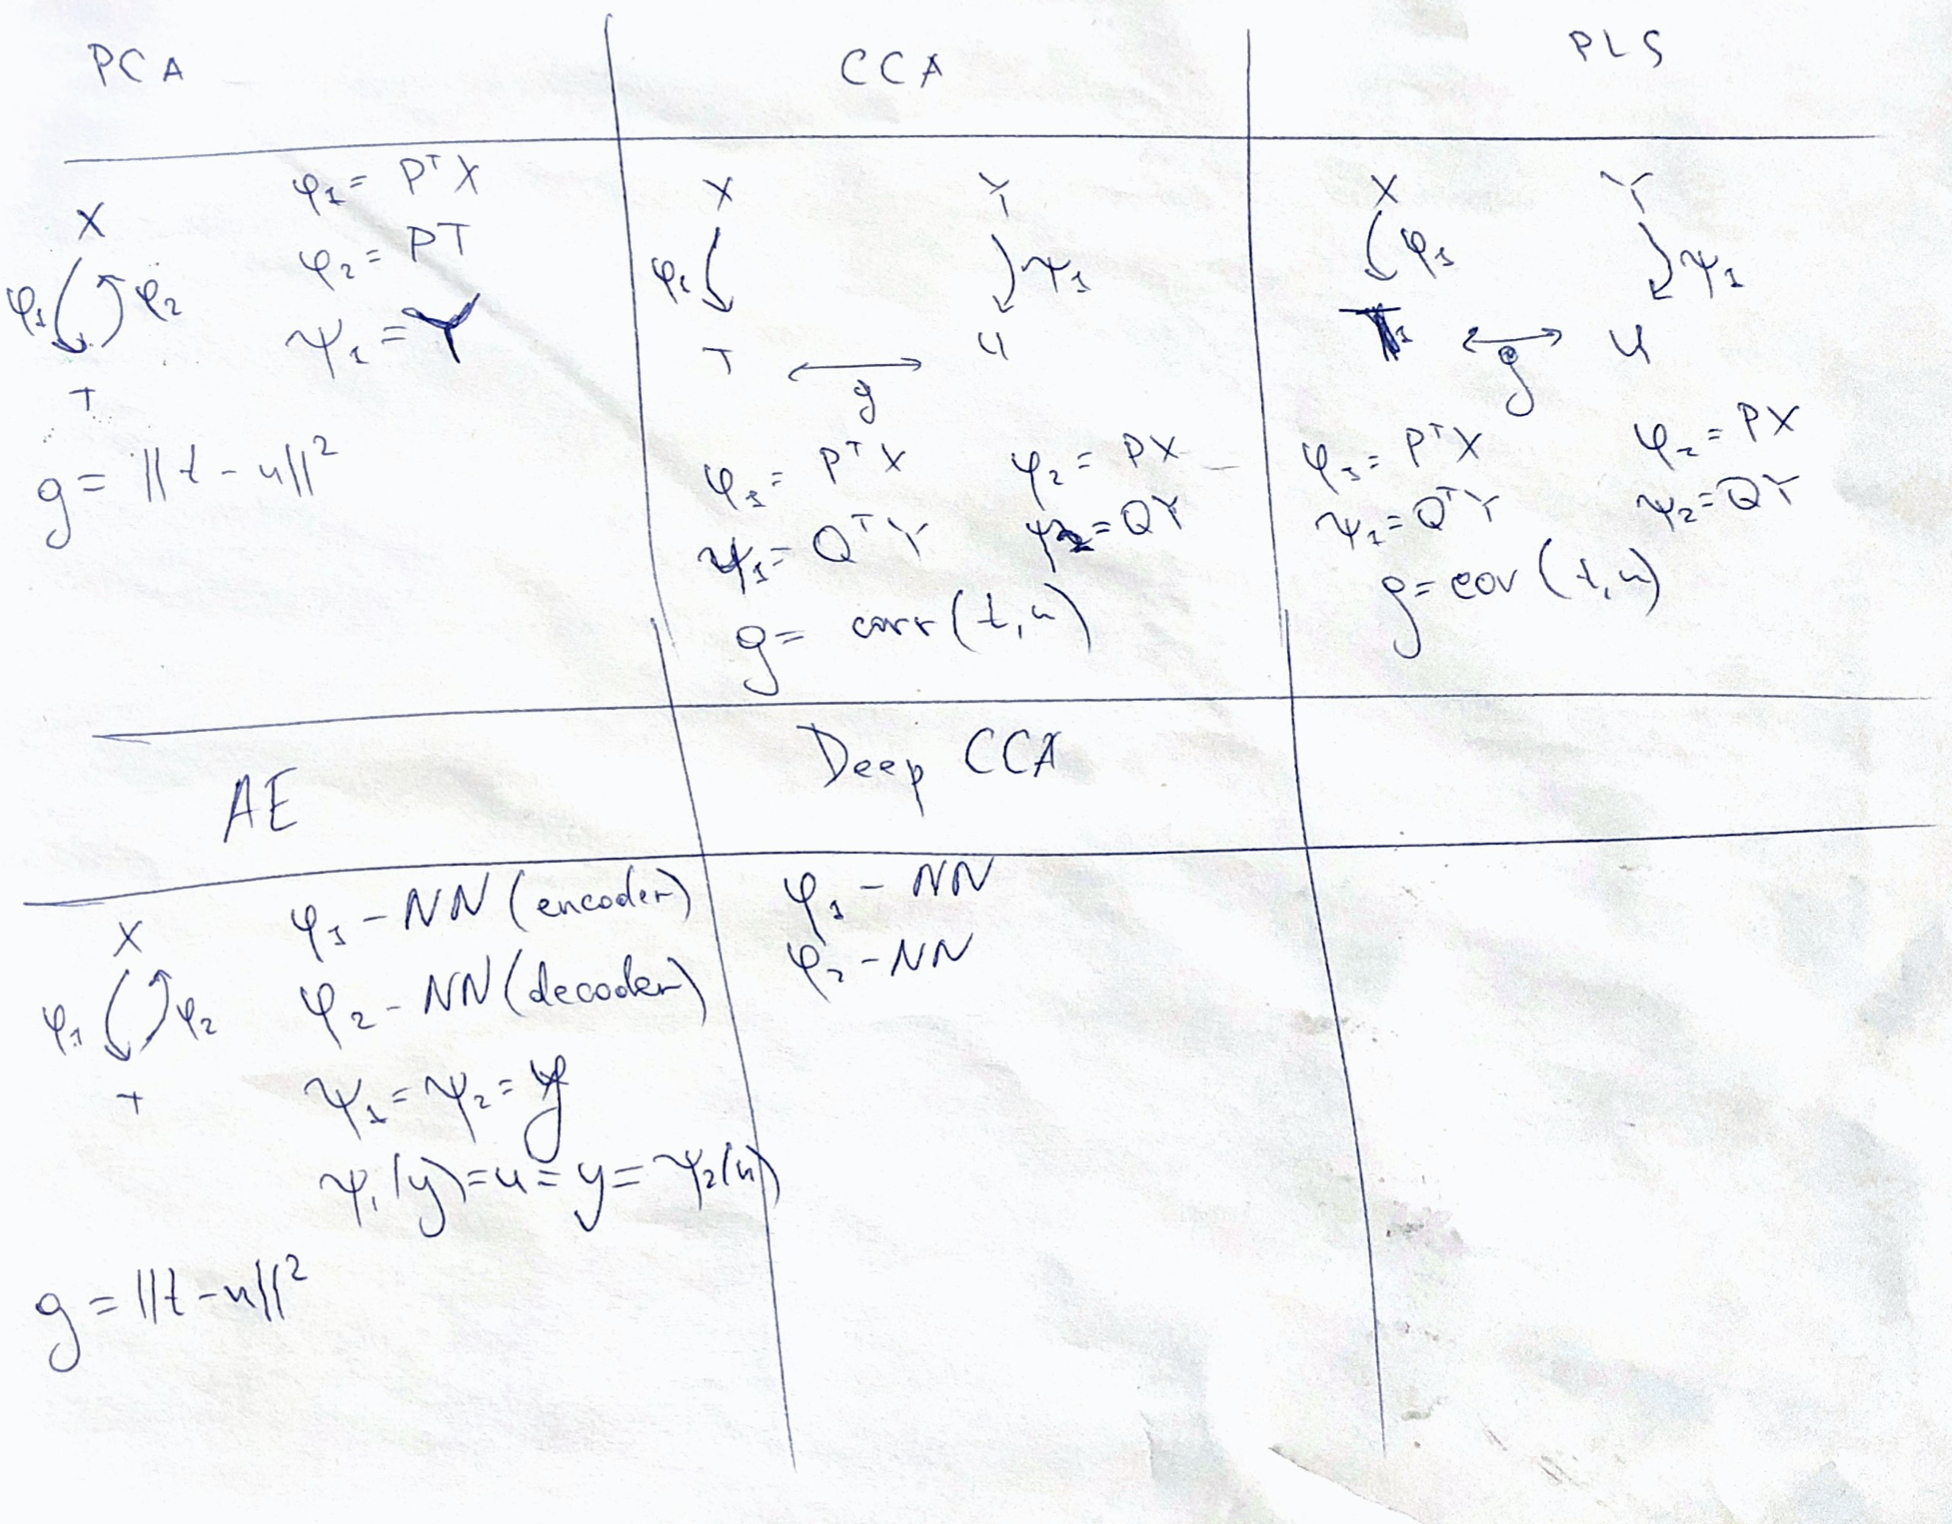
\includegraphics[width=\linewidth]{figs/ch1/Examples}
	\caption{Примеры алгоритмов, работающих по схеме \ref{ch1:eq:decoding_scheme}}
	\label{ch1:fig:PLSFigure}
\end{figure}

\subsection{Deep CCA}

Deep CCA~-- нелинейной модификация CCA. DCCA преобразует исходные данные с помощью многослойной нейронной сети таким образом, что результирующее представление становится согласованным. Предполагается, что есть $d$ слоев нейроной сети. 

Выходом первого слоя для экземпляра $\bx$ будет $\mathbf{h}_1 = s(\bW^{1}_{\bx}\bx + \bb^{1}_{\bx}) \in \mathbb{R}^{c_1}$, где $\bW_{\bx}^{1} \in \mathbb{R}^{c_1 \times m}$~-- матрица весов, $\bb_{x}^{1} \in \mathbb{R}^{c_1}$~-- вектор смещения, $s: \mathbb{R} \to \mathbb{R}$~-- нелинейная функция, которая действует покомпонентно. Далее выход первого слоя используется для вычисления выхода второго слоя $\mathbf{h}_{2} = s(\bW^{2}_{\bx}\mathbf{h}_{1} + \bb^{2}_{\bx}) \in \mathbb{R}^{c_2}$ и так далее до тех пор пока не будет найдено конечное представление $\varphi_e(\bx) = s(\bW^{d}_{\bx}\mathbf{h}_{d-1} + \bb^{d}_{\bx}) \in \mathbb{R}^{p}$. Аналогично находится представление для $\by$: $\psi_e(\by) = s(\bW^{d}_{\by}\mathbf{h}_{d-1} + \bb^{d}_{\by}) \in \mathbb{R}^{p}.$

Обозначим $\theta_{\bx}$, $\theta_{\by}$~-- параметры для функций кодирования, то есть матрицы весов и векторы смещений. Оптимальные параметры $\theta_{\bx}^{*}$, $\theta_{\by}^{*}$ находятся из задачи оптимизации:
\begin{equation}
(\theta_{\bx}^{*}, \theta_{\by}^{*}) = \argmax _{(\theta_{\bx}, \theta_{\by})} [g(\varphi_e(\bX; \theta_{\bx}), \psi_e(\bY; \theta_{2}))] = \argmax _{(\theta_{\bx}, \theta_{\by})} [corr(\varphi_e(\bX; \theta_{\bx}), \psi_e(\bY; \theta_{2}))].
\end{equation}

%%%%%%%%%%%%%%%%%%%%%%%%%%%%%%%%%%%%%%%%%%%%%%%%
\section{Вычислительный эксперимент}
%%%%%%%%%%%%%%%%%%%%%%%%%%%%%%%%%%%%%%%%%%%%%%%%

Временные ряды электроэнергии состоят из почасовых записей (52512 наблюдений). 
Строка матрицы~$\bX$~--– локальная история сигнала за одну неделю $n = 24 \times 7$. Строка матрицы~$\bY$~--- локальный прогноз потребления электроэнергии в следующие 24 часа $r = 24$. В этом случае матрицы~$\bX$ и~$\bY$ являются авторегрессионными матрицами.

Вычислительный эксперимент также проводился на данных электрокортикограмм (ECoG) из проекта NeuroTycho~\cite{shimoda2012decoding}.
Данные ECoG состоят из 32-канальных сигналов напряжения, снятых с головного мозга.
Цель состоит в предсказании по входному сигналу ECoG 3D позиции рук в последующие моменты времени.
Исходные сигналы напряжения преобразуются в пространственно-временное представление с помощью вейвлет-преобразования с материнским вейвлетом Морле.
Процедура извлечения признаков из исходных данных подробно описана в~\cite{chao2010long,eliseyev2016penalized}.
Описание исходного сигнала в каждый момент времени имеет размерность 32 (каналы) $\times $ 27 (частоты) = 864.
Каждый объект представляет собой локальный отрезок времени длительностью $\Delta t = 1s$. Временной шаг между объектами $\delta t = 0.05 s$.
Матрицы имеют размеры $\bX \in \bbR^{18900 \times 864}$ и $\bY \in \bbR^{18900 \times 3k}$, где $k$ - число отсчётов времени прогнозирования.
Данные разбиты на тренировочную и тестовую части в соотношении 0,67. 
Пример исходных сигналов мозга и соответствующей траектории руки показан на рисунке~\ref{ch2:fig:ecog_data}.

\begin{figure}
	\centering
	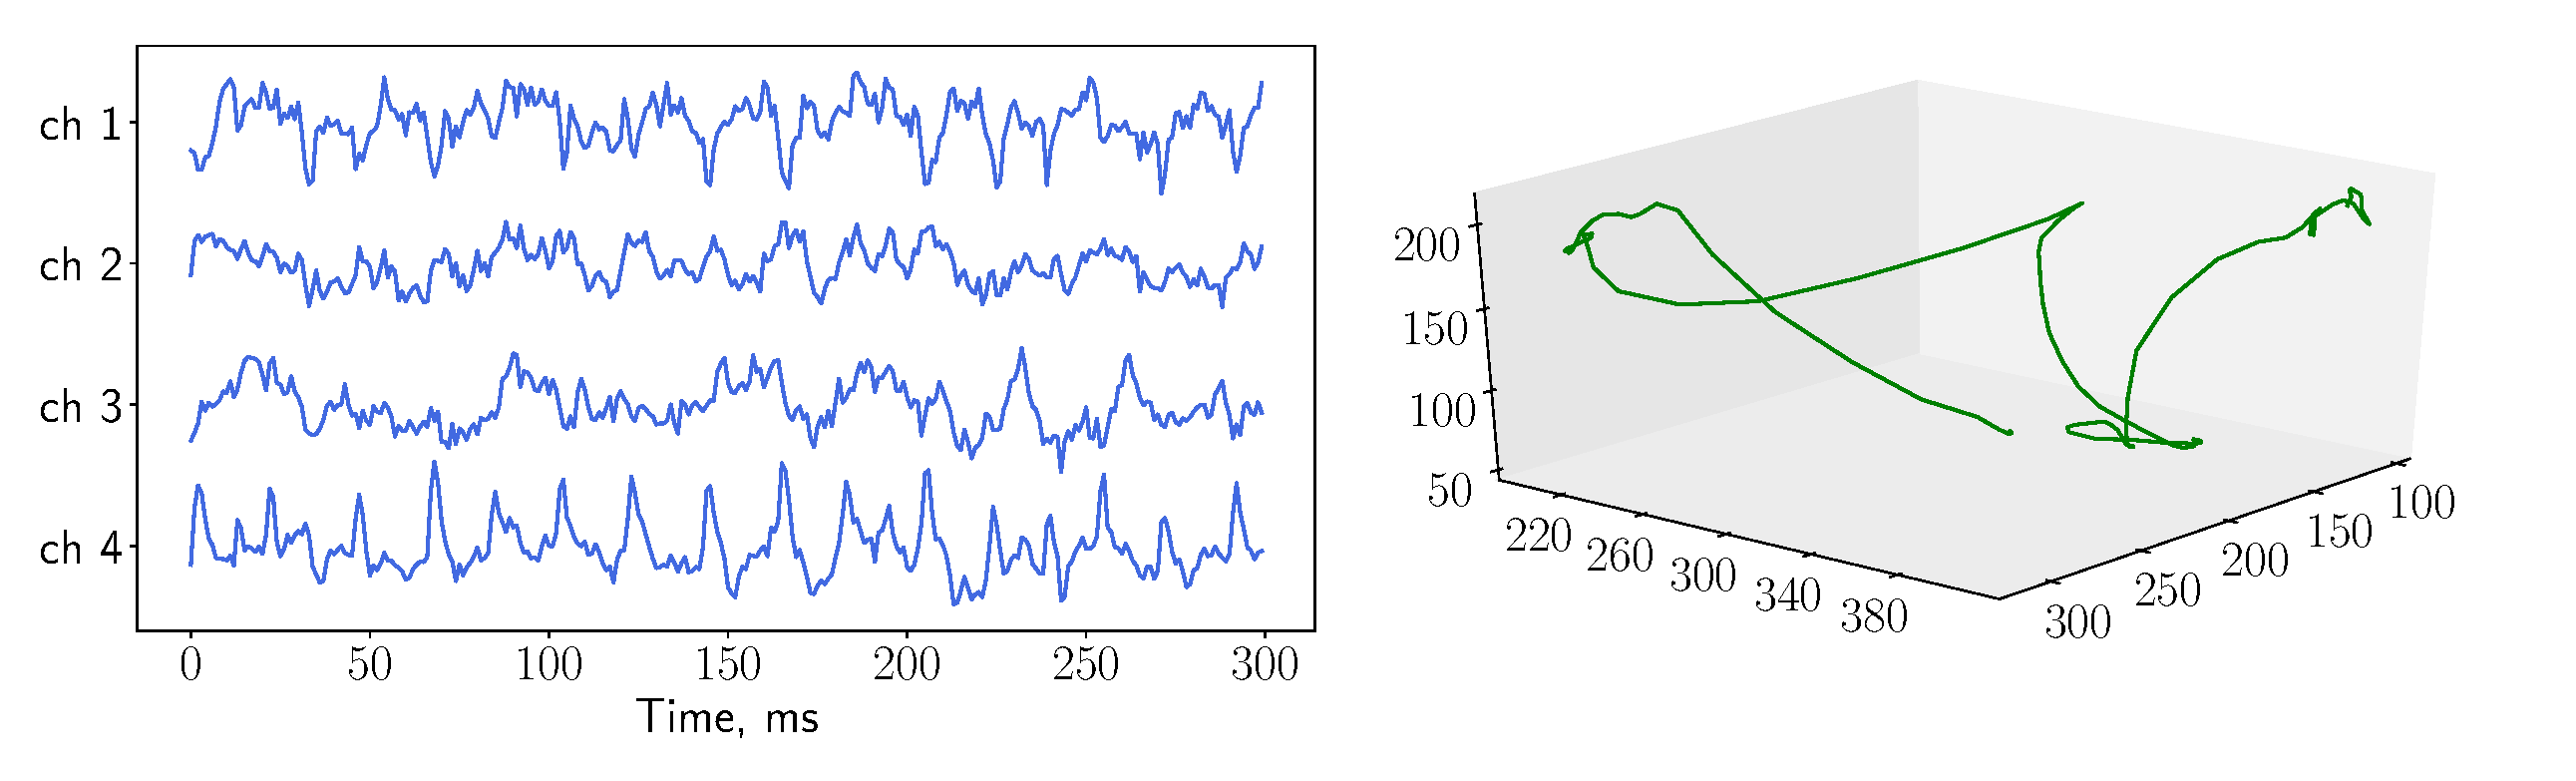
\includegraphics[width=\linewidth]{figs/ch2/ecog_data}
	\caption{Сигналы мозга (левый график) и 3D координаты руки (правый график)}
	\label{ch1:fig:ecog_data}
\end{figure}

Введём среднеквадратичную ошибку для некоторых матриц $\mathbf{A} = [a_{ij}]$ и $\mathbf{B} = [b_{ij}]$
\[
\text{MSE} (\mathbf{A}, \mathbf{B}) = \sum_{i,j} (a_{ij} - b_{ij})^2.
\]
Для оценивания качества аппроксимации вычисляется значение нормированной среднеквадратичной ошибки
\begin{equation}
\text{NMSE}(\bY,  \mathbf{\hat{Y}}) = \frac{\text{MSE} (\bY, \mathbf{\hat{Y}})}{\text{MSE} (\bY, \mathbf{\bar{Y}})},
\label{ch1:eq:nmse}
\end{equation}
где $\mathbf{\hat{Y}}$~--- прогноз модели, $\mathbf{\bar{Y}}$~--- константный прогноз средним значением по столбцам матрицы.

\subsection*{Данные потребления электроэнергии}

Для нахождения оптимальной размерности $l$ латентного пространства все данные потребления электроэнергии были разбиты на обучающую и валидационную части. 
Обучающая выборка состоит из $700$ объектов, валидационная из $370$. Зависимость нормированной квадратичной ошибки~\eqref{ch1:eq:nmse} от размерности $l$ латентного пространства представлена на Рис.~\ref{ch1:fig:energy_n_comp}. 
Сначала ошибка резко падает при увеличении размерности скрытого пространства, а затем стабилизируется.

\begin{figure}[ht]
	\centering
	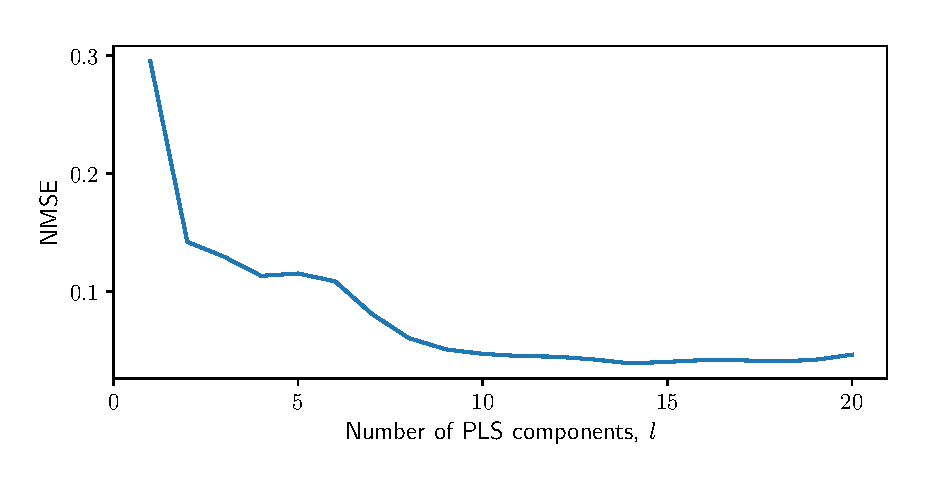
\includegraphics[width=0.75\linewidth]{figs/ch1/energy_n_comp}
	\caption{Прогноз потребления электроэнергии алгоритмом PLS при размерности латентного пространства $l$=14}
	\label{ch1:fig:energy_n_comp}
\end{figure}

Минимальная ошибка наблюдается при $l=14$. 
Построим прогноз потребления электроэнергии при данном $l$. 
Результат аппроксимации изображен на Рис.~\ref{ch1:fig:energy_prediction}. Алгоритм PLS восстановил авторегрессионную зависимость и обнаружил дневную сезонность.

\begin{figure}[ht]
	\centering
	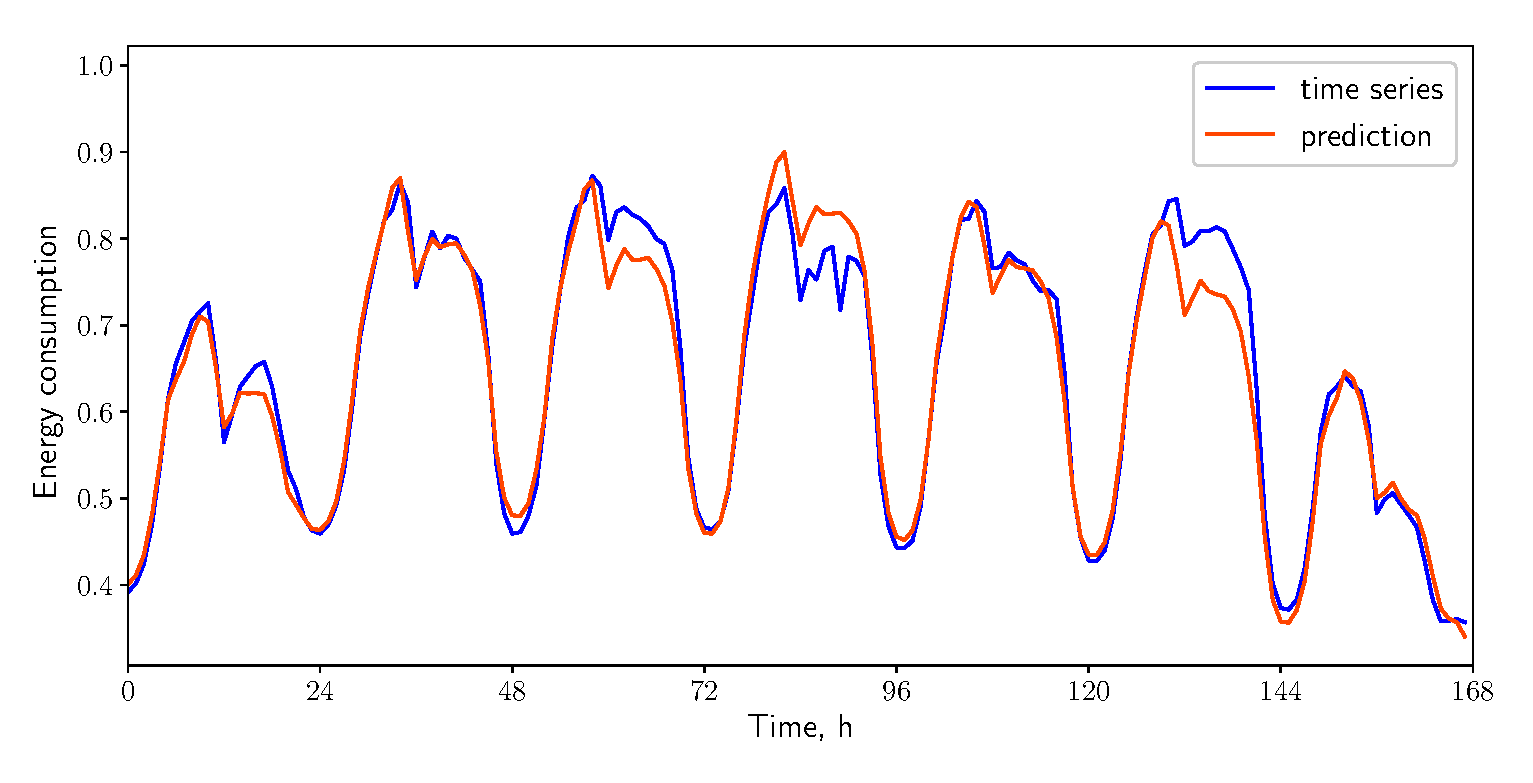
\includegraphics[width=0.95\textwidth]{figs/ch1/energy_prediction}
	\caption{Зависимость ошибки от размерности латентного пространства для данных потребления электроэнергии}
	\label{ch1:fig:energy_prediction}
\end{figure}

\subsection*{Данные электрокортикограммы}

На Рис.~\ref{ch1:fig:ecog_n_comp} представлена зависимость нормированной квадратичной ошибки~\eqref{ch1:eq:nmse} от размерности латентного пространства. Ошибка аппроксимации меняется незначительно при $l > 5$.
Таким образом совместное описание пространственно-временного спектрального представления объектов и пространственного положения руки может быть представлено вектором размерности $l \ll n$.
Зафиксируем $l = 5$. 
Пример аппроксимации положения руки изображен на Рис.~\ref{ch1:fig:ecog_prediction}. 
Сплошными линиями изображены истинные координаты руки по всем осям, пунктирными линиями показана аппроксимация методом PLS.
 
\begin{figure}[ht]
	\centering
	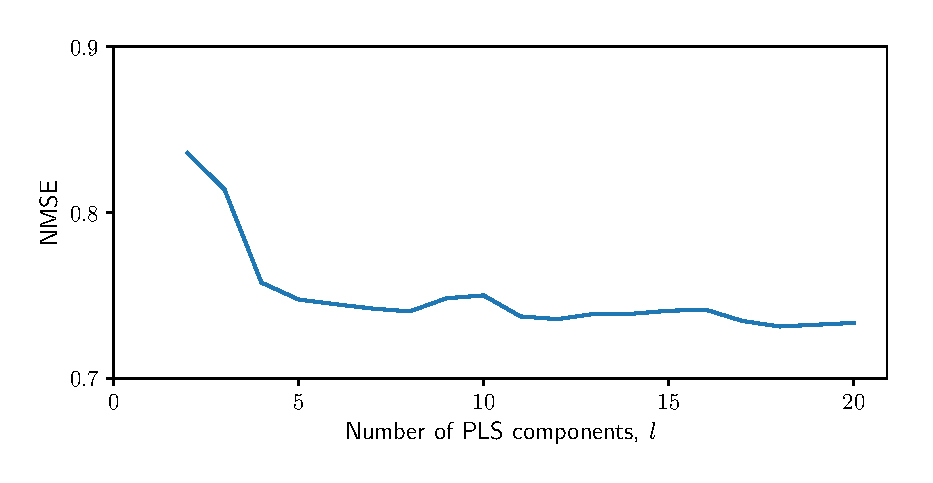
\includegraphics[width=0.75\linewidth]{figs/ch1/ecog_n_comp}	
	\caption{Зависимость ошибки от размерности латентного пространства для данных ECoG}
	\label{ch1:fig:ecog_n_comp}
\end{figure}

\begin{figure}[ht]
	\centering
	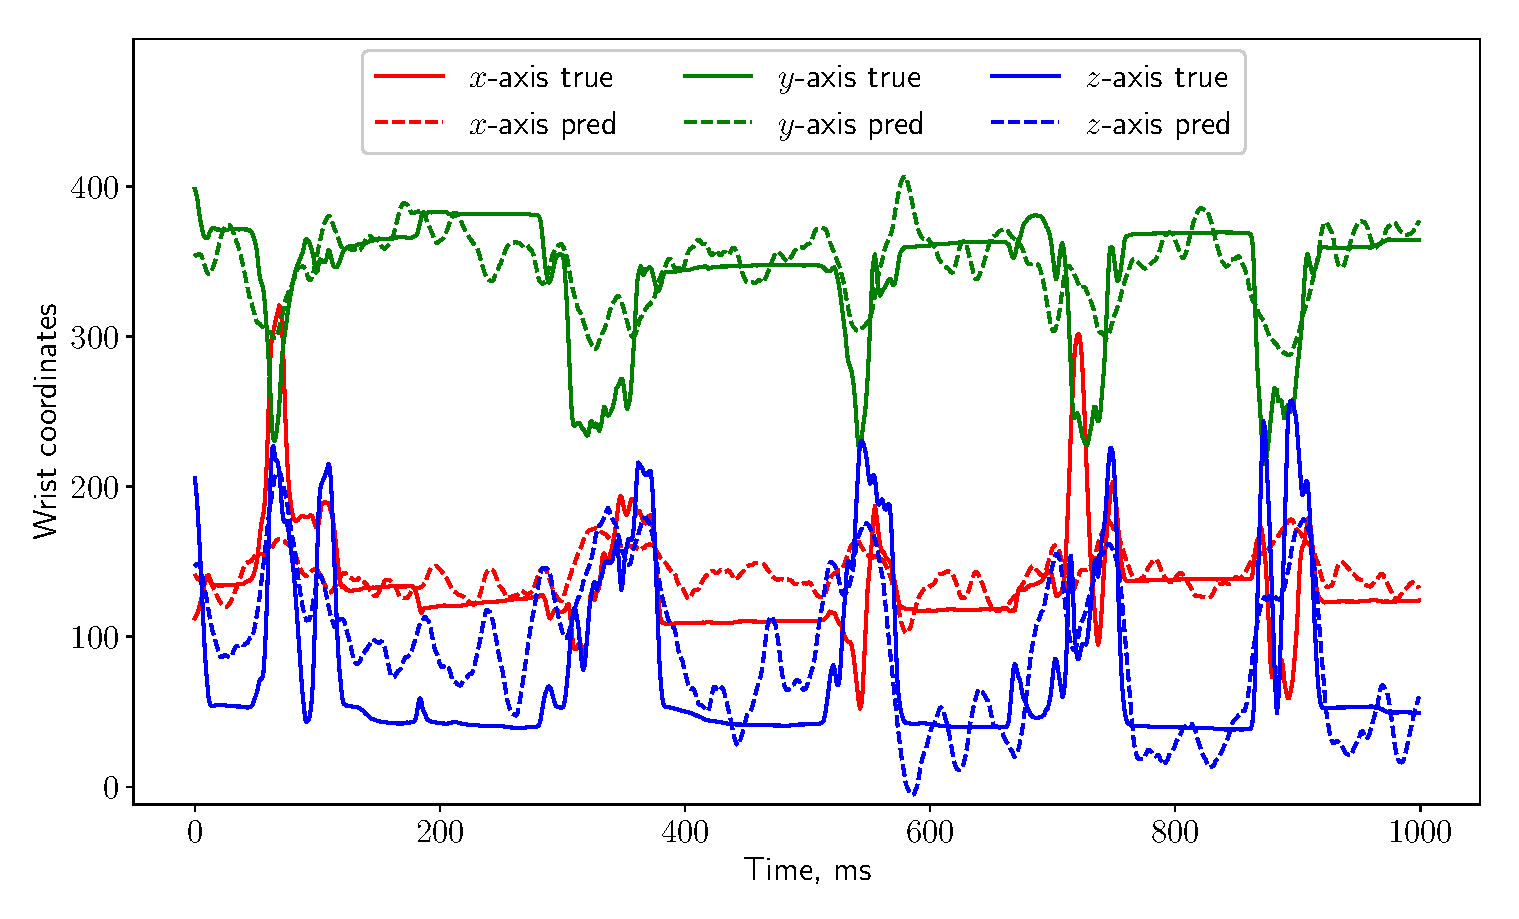
\includegraphics[width=\textwidth]{figs/ch1/ecog_prediction}
	\caption{Прогноз движения руки по данным ECoG алгоритмом PLS при размерности латентного пространства $l=5$}
	\label{ch1:fig:ecog_prediction}
\end{figure}



\newpage{}
\chapter{Выбор признаков в задаче декодирования сигналов}
\label{ch:qpfs}

Задача выбора признаков заключается в поиске оптимального подмножества~$\cA \subset \{ 1, \dots, n \}$ индексов признаков среди всех возможных $2^n - 1$ вариантов. 
Существует взаимооднозначное отображение между подмножеством $\cA$ и булевым вектором~$\ba \in \{0, 1\}^n$, компоненты которого указывают, выбран ли признак. 
Для нахождения оптимального вектора~$\ba$ введем функцию ошибки выбора признаков~$S(\ba, \bX, \bY)$. 
Проблема выбора признаков принимает вид:
\begin{equation}
	\ba = \argmin_{\ba' \in \{0, 1\}^n} S(\ba', \bX, \bY).
	\label{ch3:eq:feature_selection}
\end{equation}
Целью выбора признаков является построение функции~$S (\ba, \bX, \bY)$. Конкретные примеры данной функции для рассматриваемых методов выбора признаков приведены ниже и обобщены в таблице~\ref{ch3:tbl:summary}.

Задача~\eqref{ch3:eq:feature_selection} имеет дискретную область определения~$\{0, 1\}^n$. Для решения данной задачи применяется релаксация задачи~\eqref{ch3:eq:feature_selection} к непрерывной области определения~$[0, 1]^n$. Релаксированная задача выбора признаков имеет следующий вид:
\begin{equation}
	\bz = \argmin_{\bz' \in [0, 1]^n} S(\bz', \bX, \bY).
	\label{ch3:eq:relaxed_feature_selection}
\end{equation}

Здесь компоненты вектора~$\bz$~--- значения нормированных коэффициентов значимости признаков.
Сначала решается задача~\eqref{ch3:eq:relaxed_feature_selection}, для получения вектора значимостей~$\bz$. 
Затем решение~\eqref{ch3:eq:feature_selection} восстанавливается с помощью отсечения по порогу следующим образом:
\begin{equation}
	\ba = [a_j]_{j=1}^n, \quad 
	a_j = \begin{cases}
		1, & z_j > \tau; \\
		0, & \text{в противном случае}.
	\end{cases}
	\label{ch3:eq:feature_threshold}
\end{equation}
$\tau$~--- гиперпараметр, который может быть подобран вручную или выбран с помощью кросс-валидации. 

Как только решение~$\ba$ задачи~\eqref{ch3:eq:feature_selection} получено, задача~\eqref{ch1:eq:l2_loss_function} принимает вид:
\begin{equation*}
	\mathcal{L}(\bTheta_{\cA}, \bX_{\cA}, \bY) = {\left\| \mathbf{Y} - \bX_{\cA}\bTheta_{\cA} \right\| }_2^2 \rightarrow\min_{\bTheta_{\cA}},
\end{equation*}
где индекс~$\cA$ обозначает подматрицу со столбцами, индексы которых содержатся в~$\cA$.

%%%%%%%%%%%%%%%%%%%%%%%%%%%%%%%%%%%%%%%%%%%%%%%%
\section{Выбор признаков с помощью квадратичного программирования}
\label{sec:ch3:qpfs_feature_selection}
%%%%%%%%%%%%%%%%%%%%%%%%%%%%%%%%%%%%%%%%%%%%%%%%

Если между столбцами матрицы исходных объектов~$\bX$ существует линейная зависимость, то решение задачи линейной регрессии
\begin{equation}
	\| \bupsilon - \bX \btheta\|_2^2 \rightarrow\min_{\btheta \in \bbR^{n}}.
	\label{ch3:eq:linear_regression}
\end{equation}
оказывается неустойчивым. 
Методы выбора признаков находят подмножество~$ \cA \in \{1, \dots, n\}$ оптимальных столбцов матрицы~$\bX$. 

Метод QPFS~\cite{rodriguez2010quadratic} выбирает некоррелированные признаки, релевантные целевому вектору~$\bupsilon$.
Чтобы формализовать этот подход, введем две функции: $\text{Sim}(\bX)$ и $\text{Rel}(\bX, \bupsilon)$. 
$\text{Sim}(\bX)$ контролирует избыточность между признаками, $\text{Rel}(\bX, \bupsilon)$ содержит релевантности между каждым признаком и целевым вектором. 
Мы хотим минимизировать функцию Sim и максимизировать Rel одновременно.

QPFS предлагает явный способ построения функций Sim и Rel. 
Метод минимизирует следующую функцию ошибки
\begin{equation}
	\underbrace{\bz^{\T} \bQ \bz}_{\text{Sim}} - \alpha \cdot \underbrace{\vphantom{()} \mathbf{b}^{\T} \bz}_{\text{Rel}} \rightarrow \min_{\substack{\bz \in \bbR^n_+ \\ \|\bz\|_1=1}}.
	\label{ch3:eq:qpfs_problem}
\end{equation}
Элементы матрицы парных взаимодействий~$\bQ \in \bbR^{n \times n}$ содержат коэффициенты попарного сходства между признаками. 
Вектор релевантностей признаков~$\mathbf{b} \in \bbR^n$ выражает сходство между каждым признаком и целевым вектором~$\bupsilon$.
Нормированный вектор~$\bz$ отражает значимость каждого признака. 
Функция ошибки~\eqref{ch3:eq:qpfs_problem} штрафует зависимые признаки функцией Sim и штрафует признаки, не релевантные к целевой переменной функцией Rel. 
Параметр~$\alpha$ позволяет контролировать компромисс между Sim и Rel.
Авторы оригинальной статьи QPFS~\cite{rodriguez2010quadratic} предложили способ выбора~$\alpha$, чтобы уравновесить вклад членов $\text{Sim}(\bX)$ и $\text{Rel}(\bX, \bupsilon)$

\begin{equation*}
	\alpha = \frac{\overline{\bQ}}{\overline{\bQ} + \overline{\bb}}, \quad \text{где}\,\,\overline{\bQ} = \text{mean} (\bQ), \,\,\, \overline{\bb}= \text{mean} (\bb).
\end{equation*}
Чтобы выделить оптимальное подмножество признаков, применяется отсечение по порогу~\eqref{ch3:eq:feature_threshold}.

Для измерения сходства используется выборочный коэффициент корреляции Пирсона между парами признаков для функции Sim, и между признаками и целевым вектором для функции Rel:
\begin{equation}
	\bQ = \left[|\text{corr}(\bchi_i, \bchi_j)|\right]_{i,j=1}^n, \quad \bb = \left[|\text{corr}(\bchi_i, \bupsilon)|\right]_{i=1}^n.
	\label{ch3:eq:qpfs_1d_qb}
\end{equation}
Здесь
\begin{equation*}
\text{corr}(\bchi, \bupsilon) = \frac{\sum_{i=1}^m(\bchi_i - \overline{\bchi})( \bupsilon_i - \overline{\bupsilon})}{\sqrt{\sum_{i=1}^m(\bchi_i - \overline{\bchi})^2\sum_{i=1}^m(\bupsilon_i - \overline{\bupsilon})^2}}.
\end{equation*}
Другие способы определения $\bQ$ и $\bb$ рассматриваются в~\cite{katrutsa2017comprehensive}. 
В работе~\cite{katrutsa2017comprehensive} показано, что метод QPFS превосходит многие существующие методы выбора признаков на различных внешних критериях качества.

Задача~\eqref{ch3:eq:qpfs_problem} является выпуклой, если матрица~$\bQ$ является неотрицательно определенной. В общем случае это не всегда верно. 
Чтобы удовлетворить этому условию спектр матрицы~$\bQ$ смещается, и матрица~$\bQ$ заменяется на $\bQ - \lambda_{\text{min}} \mathbf{I}$, где $\lambda_{\text{min}} $ является минимальным собственным значением~$\bQ$.

%%%%%%%%%%%%%%%%%%%%%%%%%%%%%%%%%%%%%%%%%%%%%%%%
\section{Методы выбора признаков для случая векторной целевой переменной}
\label{sec:ch3:mqpfs_feature_selection}
%%%%%%%%%%%%%%%%%%%%%%%%%%%%%%%%%%%%%%%%%%%%%%%%

В данном разделе описаны предлагаемые методы выбора признаков для случая векторной целевой переменной.
В этом случае компоненты целевой переменной могут коррелировать между собой. 
Предлагаются методы, учитывающие зависимости как в исходном, так и в целевом пространствах.

\textbf{Агрегация релевантностей целевых векторов.}
В работе~\cite{motrenko2018multi}, чтобы применить метод QPFS к векторному случаю ($r > 1$), релевантности признаков агрегируются по всем $r$ компонентам целевой переменной. 
Член $\text{Sim}(\bX)$ остаётся без изменений, матрица парных взаимодействий~$\bQ$ определяется как~\eqref{ch3:eq:qpfs_1d_qb}. 
Вектор релевантностей $\bb$ агрегируется по всем компонентам целевой переменной и определяется как
\begin{equation*}
	\bb = \left[\sum_{k=1}^r|\text{corr}(\bchi_i, \bupsilon_k)|\right]_{i=1}^n.
\end{equation*}
Недостатком такого подхода является отсутствие учёта зависимостей в столбцах матрицы~$\bY$. Рассмотрим следующий пример:
\begin{equation*}
	\bX = [\bchi_1, \bchi_2, \bchi_3], \quad \bY = [\underbrace{\bupsilon_1, \bupsilon_1, \dots, \bupsilon_1}_{r-1}, \bupsilon_2].
\end{equation*}
Пусть матрица~$\bX$ содержит 3 столбца, матрица~$\bY$~--- $r$ столбцов, где первые $r-1$ компонент целевой переменной идентичны.
Попарные сходства признаков задаются матрицей~$\bQ$.
Матрица~$\bB$ содержит попарные сходства признаков и целевых столбцов.
Вектор~$\bb$ получен суммированием матрицы~$\bB$ по столбцами
\begin{equation}
	\bQ = \begin{bmatrix} 1 & 0 & 0\\ 0 & 1 & 0.8 \\ 0 & 0.8 & 1 \end{bmatrix}, \quad
	\bB = \begin{bmatrix} 0.4 & \dots & 0.4 & 0 \\ 0.5 & \dots & 0.5 & 0.8 \\ 0.8 & \dots & 0.8 & 0.1 \end{bmatrix}, \quad
	\bb = \begin{bmatrix} (r-1) \cdot 0.4 + 0 \\ (r-1) \cdot 0.5 + 0.8 \\ (r-1) \cdot 0.8 + 0.1 \end{bmatrix}.
	\label{ch3:eq:qpfs_example}
\end{equation}
\vspace{0.5cm} \\
Пусть необходимо выбрать только 2 признака.
В данном случае оптимальным подмножеством признаков является~$[\bchi_1, \bchi_2]$.
Признак~$\bchi_2$ предсказывает второй целевой столбец~$\bupsilon_2$, комбинация признаков~$\bchi_1, \bchi_2$ прогнозирует первый целевой столбец~$\bupsilon_1$.
Метод QPFS для~$r=2$ дает решение~$\bz = [0.37, 0.61, 0.02]$. Это совпадает с описанным решением.
Однако, если добавить коллинеарные столбцы в матрицу~$\bY$ и увеличить~$r$ до 5, то решением QPFS будет~$\bz = [0.40, 0.17, 0.43]$.
Здесь потерян признак~$\bchi_2$ и выбран избыточный признак~$\bchi_3$.
В следующих подразделах предлагаются обобщения метода QPFS, которые позволяют бороться с проблемой данного примера.

\textbf{Симметричный учёт значимости признаков и целевых переменных.}
Чтобы учесть зависимости в столбцах матрицы~$\bY$, обобщим функцию QPFS~\eqref{ch3:eq:qpfs_problem} для случая векторной целевой переменной ($r > 1$).
Добавим член~$\text{Sim}(\bY)$ и изменим член $\text{Rel}(\bX, \bY)$ следующим образом:
\begin{equation}
	\alpha_1 \cdot \underbrace{\bz_x^{\T} \bQ_x \bz_x}_{\text{Sim}(\bX)} - \alpha_2 \cdot \underbrace{\bz_x^{\T} \bB \bz_y}_{\text{Rel}(\bX, \bY)} + \alpha_3 \cdot \underbrace{\bz_y^{\T} \bQ_y \bz_y}_{\text{Sim}(\bY)} \rightarrow \min_{\substack{\bz_x \geq \bZero_n, \, \bOne_n^{\T}\bz_x=1 \\ \bz_y \geq \bZero_r, \, \bOne_r^{\T}\bz_y=1}}.
	\label{ch3:eq:symimp}
\end{equation}
Определим элементы матриц~$\bQ_x \in \bbR^{n \times n}$, $\bQ_y \in \bbR^{r \times r}$ и $\bB \in \bbR^{n \times r}$ следующим образом:
\begin{equation*}
	\bQ_x = \left[ |\text{corr}(\bchi_i, \bchi_j)| \right]_{i,j=1}^n, \quad
	\bQ_y = \left[ |\text{corr}(\bupsilon_i, \bupsilon_j)| \right]_{i,j=1}^r, \quad
	\bB =  \left[ |\text{corr}(\bchi_i, \bupsilon_j)| \right]_{\substack{i=1, \dots, n \\ j=1, \dots, r}}.
\end{equation*}
Вектор~$\bz_x$ содержит коэффициенты значимости признаков, $\bz_y$~--- коэффициенты значимости целевых векторов.
Коррелированные целевые столбцы штрафуются членом~$\text{Sim}(\bY)$ и получают более низкие значения значимости.

Коэффициенты $\alpha_1$, $\alpha_2$, и $\alpha_3$ контролируют влияние каждого члена на функцию~\eqref{ch3:eq:symimp} и удовлетворяют следующим условиям:
\begin{equation*}
	\alpha_1 + \alpha_2 + \alpha_3 = 1, \quad \alpha_i \geq 0, \, i = 1, 2, 3.
\end{equation*}
\begin{statement}
	Баланс между~$\text{Sim}(\bX)$, $\text{Rel}(\bX, \bY)$ и $\text{Sim}(\bY)$ в  задаче~\eqref{ch3:eq:symimp} достигается при:
	\begin{equation}
	\alpha_1 \propto \overline{\bQ}_y \overline{\bB}, \quad
	\alpha_2 \propto \overline{\bQ}_x \overline{\bQ}_y, \quad
	\alpha_3  \propto \overline{\bQ}_x \overline{\bB}.
	\label{ch3:eq:alpha_3}
	\end{equation}
	
\end{statement}
\begin{proof}
	Значения $\alpha_1$, $\alpha_2$, и $\alpha_3$ получаются путем решения следующих уравнений:
	\begin{align*}
	&\alpha_1 + \alpha_2 + \alpha_3 = 1, \\
	&\alpha_1 \overline{\bQ}_x = \alpha_2 \overline{\bB} = \alpha_3 \overline{\bQ}_y.
	\end{align*}
	Здесь~$\overline{\bQ}_x$, $\overline{\bB}$ и $\overline{\bQ}_y$~--- средние значения соответствующих матриц~$\bQ_x$, $\bB$ и $\bQ_y$ членов~$\text{Sim}(\bX)$, $\text{Rel}(\bX, \bY)$ и $\text{Sim}(\bY)$.
\end{proof}
Для изучения зависимости~$\text{Sim}(\bY)$ на функцию~\eqref{ch3:eq:symimp}, зафиксируем соотношение между~$\alpha_1$ и $\alpha_2$:
\begin{equation}
	\alpha_1 = \frac{(1 - \alpha_3)\overline{\bB}}{\overline{\bQ}_x + \overline{\bB}}, \quad
	\alpha_2 = \frac{(1 - \alpha_3)\overline{\bQ}_x}{\overline{\bQ}_x + \overline{\bB}}, \quad
	\alpha_3 \in [0, 1].
	\label{ch3:eq:alphas3}
\end{equation}

Применим предложенный метод к приведенному примеру~\eqref{ch3:eq:qpfs_example}.
Матрица~$\bQ$ соответствует матрице~$\bQ_x$.
Определим матрицы~$\bQ_y$ как $\text{corr}(\bupsilon_1, \bupsilon_2) = 0.2$, а все остальные элементы зададим 1.
Рисунок~\ref{ch3:fig:features_vs_alpha} показывает значение векторов значимостей признаков~$\bz_x$ и целевых векторов~$\bz_y$ в зависимости от значения коэффициента~$\alpha_3$.
Если~$\alpha_3$ мало, значимости всех целевых векторов не различимы и значимость признака~$\bchi_3$ выше значимости признака~$\bchi_2$. При увеличении~$\alpha_3$ до~$0.2$, коэффициент значимости~$\bz_{y,5}$ целевого вектора~$\bupsilon_5$ увеличивается наряду со значимостью признака~$\bchi_2$.

\begin{figure}
	\centering
	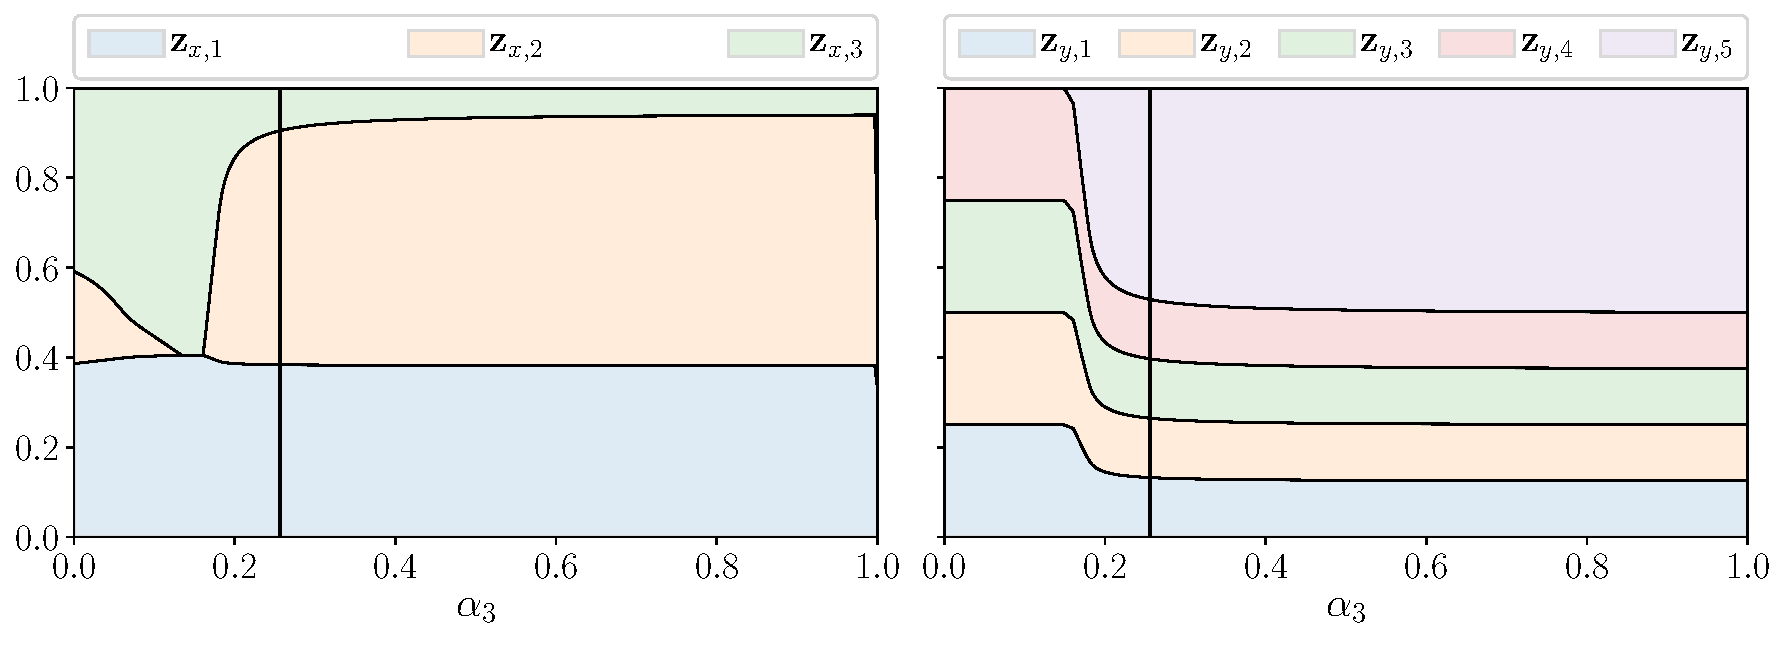
\includegraphics[width=\linewidth]{figs/ch3/features_vs_alpha.pdf}
	\caption{Значимости признаков~$\bz_x$ и целевых векторов~$\bz_y$ в зависимости от~$\alpha_3$ для рассмотренного примера}
	\label{ch3:fig:features_vs_alpha}
\end{figure}

\textbf{Минимаксная постановка задачи выбора признаков.}
Функция~\eqref{ch3:eq:symimp} является симметричной по отношению к~$\bz_x$ и $\bz_y$.
Она штрафует признаки, которые коррелированы и не имеют отношения к целевым векторам.
Кроме того, она штрафует целевые вектора, которые коррелированы между собой и недостаточно коррелируют с признаками.
Это приводит к малым значениям значимостей для целевых векторов, которые слабо коррелируют с признаками, и большим значениям для целевых векторов, которые сильно коррелируют с признаками.
Этот результат противоречит интуиции.
Цель~--- предсказать все целевые вектора, особенно те, которые слабо коррелируют с признаками. Сформулируем две взаимосвязанные задачи:
\begin{align}
	\alpha_1 \cdot \underbrace{\bz_x^{\T} \bQ_x \bz_x}_{\text{Sim}(\bX)} - \alpha_2 \cdot \underbrace{ \bz_x^{\T}\mathbf{B} \bz_y}_{\text{Rel}(\bX, \bY)} \rightarrow \min_{\substack{\bz_x \geq \bZero_n, \\ \bOne_n^{\T}\bz_x=1}},
	\label{ch3:eq:x_qpfs}\\
	\alpha_3 \cdot \underbrace{\bz_y^{\T} \bQ_y \bz_y}_{\text{Sim}(\bY)} + \alpha_2 \cdot \underbrace{ \bz_x^{\T} \mathbf{B} \bz_y}_{\text{Rel}(\bX, \bY)} \rightarrow \min_{\substack{\bz_y \geq \bZero_r,  \\ \bOne_r^{\T}\bz_y=1}}.
	\label{ch3:eq:y_qpfs}
\end{align}
Разница между~\eqref{ch3:eq:x_qpfs} и~\eqref{ch3:eq:y_qpfs} заключается в  знаке перед членом Rel.
В пространстве исходных объектов нерелевантные признаки должны иметь меньшие значения значимости.
В то же время целевые вектора, не релевантные признакам, должны иметь большую значимость.
Задачи~\eqref{ch3:eq:x_qpfs} и \eqref{ch3:eq:y_qpfs} объединяются в совместную минимакс или максмин постановку
\begin{equation}
	\min_{\substack{\bz_x \geq \bZero_n \\ \bOne_n^{\T}\bz_x=1}} 	\max_{\substack{\bz_y \geq \bZero_r \\ \bOne_r^{\T}\bz_y=1}} f(\bz_x, \bz_y), \quad \left(\text {или} \, \max_{\substack{\bz_y \geq \bZero_r \\ \bOne_r^{\T}\bz_y=1}} \min_{\substack{\bz_x \geq \bZero_n \\ \bOne_n^{\T}\bz_x=1}} f(\bz_x, \bz_y)\right),
	\label{ch3:eq:minmax}
\end{equation}
где
\begin{equation*}
	f(\bz_x, \bz_y) = \alpha_1 \cdot \underbrace{\bz_x^{\T} \bQ_x \bz_x}_{\text{Sim}(\bX)} - \alpha_2 \cdot \underbrace{\bz_x^{\T} \bB \bz_y}_{\text{Rel}(\bX, \bY)} - \alpha_3 \cdot \underbrace{\bz_y^{\T} \bQ_y \bz_y}_{\text{Sim}(\bY)}.
\end{equation*}
\begin{theorem}
	Для положительно определенной матрицы~$\bQ_x$ и $\bQ_y$, максмин и минимакс задачи~\eqref{ch3:eq:minmax} имеют одинаковое оптимальное значение.
\end{theorem}
\begin{proof}
	Введём обозначения
	\begin{equation*}
		\mathbb{C}^n = \{\bz : \bz \geq \bZero_n, \, \bOne_n^{\T}\bz=1\}, \quad \mathbb{C}^r = \{\bz : \bz \geq \bZero_r, \, \bOne_r^{\T}\bz=1\}.
	\end{equation*}
	Множества $\mathbb{C}^n$ и $\mathbb{C}^r$ компактные и выпуклые. Функция $f: \mathbb{C}^n \times \mathbb{C}^r \rightarrow \bbR$ является непрерывной. Если~$\bQ_x$ и $\bQ_y$ положительно определенны, функция~$f$ является выпукло-вогнутой. Таким образом
	$f(\cdot, \bz_y): \mathbb{C}^n \rightarrow \bbR$ выпуклая при фиксированном~$\bz_y$, а $f(\bz_x, \cdot): \mathbb{C}^r \rightarrow \bbR$ вогнута при фиксированном~$\bz_x$.
	В этом случае по теореме Неймана о минимаксе
	\begin{equation*}
		\min_{\bz_x \in \mathbb{C}^n} \max_{\bz_y \in \mathbb{C}^r} f(\bz_x, \bz_y) = \max_{\bz_y \in \mathbb{C}^r} \min_{\bz_x\in \mathbb{C}^n} f(\bz_x, \bz_y).
	\end{equation*}
\end{proof}

Для решения минимакс задачи~\eqref{ch3:eq:minmax}, зафиксируем некоторый~$\bz_x \in \mathbb{C}^n$. Для фиксированного вектора~$\bz_x$ решаем задачу
\begin{equation}
	\max_{\bz_y \in \mathbb{C}_r} f(\bz_x, \bz_y) = \max_{\substack{\bz_y \geq \bZero_r \\ \bOne_r^{\T}\bz_y=1}} \bigl[\alpha_1 \cdot \bz_x^{\T} \bQ_x \bz_x - \alpha_2 \cdot \bz_x^{\T} \bB \bz_y - \alpha_3 \cdot \bz_y^{\T} \bQ_y \bz_y \bigr].
	\label{ch3:eq:fixed_ax}
\end{equation}
Лагранжиан для данной задачи:
\begin{equation*}
	L(\bz_x, \bz_y, \lambda, \bmu) = \alpha_1 \cdot \bz_x^{\T} \bQ_x \bz_x - \alpha_2 \cdot \bz_x^{\T} \bB \bz_y - \alpha_3 \cdot \bz_y^{\T} \bQ_y \bz_y + \lambda \cdot  (\bOne_r^{\T} \bz_y - 1) + \bmu^{\T} \bz_y.
\end{equation*}
Здесь вектор множителей Лагранжа~$\bmu$, который соответствует ограничениям на неравенства $\bz_y \geq \bZero_r$, является неотрицательным.
Двойственной задачей является
\begin{equation}
	\min_{\lambda, \, \bmu \geq \bZero_r} g(\bz_x, \lambda, \bmu) = \min_{\lambda, \, \bmu \geq \bZero_r}  \left[\max_{\bz_y \in \bbR^r} L(\bz_x, \bz_y, \lambda, \bmu) \right].
	\label{ch3:eq:dual}
\end{equation}
Для задачи квадратичного программирования~\eqref{ch3:eq:fixed_ax} с положительно определенными матрицами~$\bQ_x$ и~$\bQ_y$ выполняются условия сильной двойственности. Таким образом, оптимальное значение~\eqref{ch3:eq:fixed_ax} равно оптимальному значению~\eqref{ch3:eq:dual}. Это позволяет перейти от решения задачи~\eqref{ch3:eq:minmax} к решению задачи
\begin{equation}
\min_{\bz_x \in \mathbb{C}^n, \, \lambda, \, \bmu \geq \bZero_r} g(\bz_y, \lambda, \bmu).
\label{ch3:eq:dual_maxmin}
\end{equation}

Полагая градиент~$\nabla_{\bz_y} L(\bz_x, \bz_y, \lambda, \bmu)$ равным нулю, получим оптимальное значение~$\bz_y$:
\begin{equation*}
	\bz_y = \frac{1}{2\alpha_3} \bQ_y^{-1} \left( - \alpha_2 \cdot \bB^{\T} \bz_x +\lambda \cdot \bOne_r + \bmu \right).
\end{equation*}
Двойственная функция принимает вид
\begin{multline}
	g(\bz_x, \lambda, \bmu)
	= \max_{\bz_y \in \bbR^r} L(\bz_x, \bz_y, \lambda, \bmu) =
	\bz_x^{\T} \left( - \frac{\alpha_2^2}{4\alpha_3} \cdot \bB \bQ_y^{-1} \bB^{\T} - \alpha_1 \cdot \bQ_x\right) \bz_x \\ - \frac{1}{4 \alpha_3} \lambda^2 \cdot \bOne_r^{\T} \bQ_y^{-1} \bOne_r - \frac{1}{4 \alpha_3} \cdot \bmu^{\T} \bQ_y^{-1} \bmu + \frac{\alpha_2}{2 \alpha_3} \lambda \cdot \bOne_r^{\T} \bQ_y^{-1} \bB^{\T} \bz_x \\ - \frac{1}{2 \alpha_3} \lambda \cdot \bOne_r^{\T} \bQ_y^{-1} \bmu + \frac{\alpha_2}{2 \alpha_3} \cdot \bmu^{\T} \bQ_y^{-1} \bB^{\T} \bz_x + \lambda.
	\label{ch3:eq:dual_quadratic_form}
\end{multline}
Тем самым задача~\eqref{ch3:eq:dual_maxmin} является квадратичной задачей с~$n + r + 1$ переменными.

\textbf{Несимметричный учёт значимостей признаков и целевых переменных.}
Естественным способом преодоления проблемы метода SymImp является добавление штрафа для целевых векторов, которые коррелируют с признаками.
Добавим линейный член~$\bb^{\T} \bz_y$ в член $\text{Rel}(\bX, \bY)$ следующим образом:
\begin{equation}
	\alpha_1 \cdot \underbrace{\bz_x^{\T} \bQ_x \bz_x}_{\text{Sim}(\bX)} - \alpha_2 \cdot  \underbrace{\left(\bz_x^{\T} \bB \bz_y - \bb^{\T} \bz_y \right) }_{\text{Rel}(\bX, \bY)} + \alpha_3 \cdot \underbrace{\bz_y^{\T} \bQ_y \bz_y}_{\text{Sim}(\bY)} \rightarrow \min_{\substack{\bz_x \geq \bZero_n, \, \bOne_n^{\T}\bz_x=1 \\ \bz_y \geq \bZero_r, \, \bOne_r^{\T}\bz_y=1}}.
	\label{ch3:eq:asymimp}
\end{equation}
\begin{statement}
	Пусть вектор $\bb$ равен
	\begin{equation*}
	b_j = \max_{i=1, \dots n} [\bB]_{i, j}.
	\end{equation*}
	Тогда значение коэффициентов значимостей вектора~$\bz_y$ будут неотрицательными в~$\text{Rel}(\bX, \bY)$ для задачи~\eqref{ch3:eq:asymimp}.
\end{statement}
\begin{proof}
	Утверждение следует из факта
	\[
	\sum_{i=1}^n  z_i b_{ij} \leq \left(\sum_{i=1}^n z_i \right)\max_{i=1, \dots n} b_{ij} = \max_{i=1, \dots n} b_{ij},
	\]
	где $z_i \geq 0$ и $\sum_{i=1}^n z_i = 1$.
\end{proof}
Следовательно, функция~\eqref{ch3:eq:asymimp} штрафует в меньшей мере признаки, которые имеют отношение к целевым векторам, и целевые вектора, которые недостаточно коррелированы с признаками.
\begin{statement}
	Баланс между членами~$\text{Sim}(\bX)$, $\text{Rel}(\bX, \bY)$ и $\text{Rel}(\bX, \bY)$ для задачи~\eqref{ch3:eq:asymimp} достигается при следующих коэффициентах:
	\begin{equation*}
		\alpha_1 \propto \overline{\bQ}_y \left( \overline{\bb} - \overline{\bB}\right), \quad
		\alpha_2 \propto \overline{\bQ}_x \overline{\bQ}_y, \quad
		\alpha_3  \propto \overline{\bQ}_x \overline{\bB}.
	\end{equation*}
\end{statement}
\begin{proof}
	Необходимые значения~$\alpha_1$, $\alpha_2$, и $\alpha_3$ являются решением следующей системы уравнений:
	\begin{align}
		&\alpha_1 + \alpha_2 + \alpha_3 = 1, \\
		&\alpha_1 \overline{\bQ}_x = \alpha_2 \overline{\bB}, \label{ch3:eq:asymimp_balance1}\\
		&\alpha_2 \left(\overline{\bb} - \overline{\bB} \right) = \alpha_3 \overline{\bQ}_y.
		\label{ch3:eq:asymimp_balance2}
	\end{align}
	Здесь, в~\eqref{ch3:eq:asymimp_balance1} уравновешены $\text{Sim}(\bX)$ с первым слагаемым~$\text{Rel}(\bX, \bY)$, а в~\eqref{ch3:eq:asymimp_balance2} уравновешены $\text{Sim}(\bY)$  с~$\text{Rel}(\bX, \bY)$.
\end{proof}
\begin{statement}
	Для случая $r=1$, предложенные функции~\eqref{ch3:eq:symimp},~\eqref{ch3:eq:minmax} и~\eqref{ch3:eq:asymimp} совпадают с оригинальным методом QPFS~\eqref{ch3:eq:qpfs_problem}.
	
	\begin{proof}
		Если $r$ равно 1, то $\bQ_y = q_y$~--- скаляр, $\bz_y = 1$ и $\bB = \bb$. Задачи~\eqref{ch3:eq:symimp},~\eqref{ch3:eq:minmax} и~\eqref{ch3:eq:asymimp} принимают вид
		\begin{equation*}
		\alpha_1 \cdot \bz_x^{\T} \bQ_x \bz_x - \alpha_2 \cdot \bz_x^{\T} \bb \rightarrow \min_{\bz_x \geq \bZero_n, \, \bOne_n^{\T}\bz_x=1} .
		\end{equation*}
		При $\alpha = \frac{\alpha_2}{\alpha_1 + \alpha_2}$ последняя задачи принимает вид~\eqref{ch3:eq:qpfs_problem}.
	\end{proof}
\end{statement}

Таблица~\ref{ch3:tbl:summary} демонстрирует основные идеи и функции ошибок для каждого метода. 
RelAgg является базовой стратегией и не учитывает корреляции в целевом пространстве.
SymImp штрафует попарные корреляции между целевыми векторами.
MinMax более чувствителен к целевым векторам, которые трудно предсказать.
Стратегия Asymimp добавляет линейный член к функции SymImp, чтобы сделать вклад признаков и целевых векторов асимметричным.

\begin{table}[ht]
	\centering
	\caption{Обзор предлагаемых обобщений метода QPFS для векторной целевой переменной}
	\small{
		\begin{tabular}{c|c|c}
			\hline
			Метод & Идея & Функция ошибки $S(\bz | \bX, \bY)$ \\
			\hline && \\ [-.5em]
			RelAgg & $\min \bigl[ \text{Sim}(\bX) - \text{Rel}(\bX, \bY) \bigr] $ & $\min\limits_{\bz_x} \bigl[ (1 - \alpha) \cdot \bz_x^{\T} \bQ_x \bz_x - \alpha \cdot \bz_x^{\T} \bB \bOne_r \bigr] $ \\ &&\\[-.5em]
			SymImp & $\begin{aligned} \min \, \bigl[ \text{Sim}(\bX) & - \text{Rel}(\bX, \bY) \\ & + \text{Sim}(\bY) \bigr] \end{aligned}$ & $ \min\limits_{\bz_x, \, \bz_y} \left[ \alpha_1 \cdot \bz_x^{\T} \bQ_x \bz_x - \alpha_2 \cdot \bz_x^{\T} \bB \bz_y + \alpha_3 \cdot \bz_y^{\T} \bQ_y \bz_y \right] $\\ &&\\ [-.5em]
			MinMax & $\begin{aligned} &\min \, \bigl[ \text{Sim}(\bX) - \text{Rel}(\bX, \bY) \bigr]  \\ & \max \bigl[\text{Rel}(\bX, \bY) + \text{Sim}(\bY) \bigr] \end{aligned}$ & $	\min\limits_{\bz_x} 	\max\limits_{\bz_y} \bigl[\alpha_1 \cdot \bz_x^{\T} \bQ_x \bz_x - \alpha_2 \cdot \bz_x^{\T} \bB \bz_y - \alpha_3 \cdot \bz_y^{\T} \bQ_y \bz_y \bigr]$ \\ &&\\ [-.5em]
			AsymImp & $\begin{aligned} & \min \, \bigl[ \text{Sim}(\bX) - \text{Rel}(\bX, \bY) \bigr]\\ &  \max \bigl[\text{Rel}(\bX, \bY) + \text{Sim}(\bY) \bigr] \end{aligned}$ & $\min\limits_{\bz_x, \bz_y} \bigl[ \alpha_1 \cdot \bz_x^{\T} \bQ_x \bz_x - \alpha_2 \cdot \left(\bz_x^{\T} \bB \bz_y - \bb^{\T} \bz_y \right) + \alpha_3 \cdot \bz_y^{\T} \bQ_y \bz_y \bigr]$\\ 
			\hline
	\end{tabular}}
	\label{ch3:tbl:summary}
\end{table}


%%%%%%%%%%%%%%%%%%%%%%%%%%%%%%%%%%%%%%%%%%%%%%%%
\section{Анализ методов учета значимостей целевых переменных}
\label{sec:ch3:exp_mqpfs}
%%%%%%%%%%%%%%%%%%%%%%%%%%%%%%%%%%%%%%%%%%%%%%%%

\textbf{Внешние критерии качества.} Для оценки предложенных методов выбора признаков, введём критерии оценки качества выбранного подмножества признаков.
Определим коэффициент мультикорреляции как среднее значение коэффициента множественной корреляции следующим образом:
\begin{equation*}
R^2 = \frac{1}{r} \text{tr} \left( \bC^{\T} \mathbf{R}^{-1} \bC \right), \quad \text{где }\bC = [ \text{corr}(\bchi_i, \bupsilon_j)]_{\substack{i=1, \dots, n \\ j=1, \dots, r}}, \,\, \mathbf{R} = [ \text{corr}(\bchi_i, \bchi_j)]_{i, j = 1}^n.
\end{equation*}
Этот коэффициент принимает значение между 0 и 1. Большее значение~$R^2$ соответствует лучшему подмножеству признаков.

Нормированная среднеквадратичная ошибка (sRMSE) отображает качество прогнозирования модели. Оценка sRMSE считается на тренировочной и тестовой выборке.
\begin{equation*}
\text{sRMSE}(\bY, \widehat{\bY}_{\ba}) = \sqrt{\frac{\text{MSE} (\bY, \widehat{\bY}_{\ba})}{\text{MSE} (\bY, \overline{\bY})}} =  \frac{\| \bY - \widehat{\bY}_{\ba} \|_2}{\| \bY - \overline{\bY} \|_2}.
\end{equation*}
Здесь $\widehat{\bY}_{\ba} = \bX_{\ba} \bTheta_{\ba}^{\T}$~--- прогноз модели, $\overline{\bY}$~--- предсказание константной модели, полученное усреднением целевой переменной по всем объектам.
Данный показатель на тестовой выборке необходимо минимизировать.

Байесовский информационный критерий (BIC)~--- компромисс между качеством предсказания и размером выбранного подмножества признаков~$\|\ba\|_0 = \#\{j: a_j \neq 0\}= \sum_{j=1}^n a_j$:
\begin{equation*}
\text{BIC} = m \ln \left( \text{MSE} ( \bY, \widehat{\bY}_{\ba})\right) + \| \ba \|_0 \cdot \ln m.
\end{equation*}
Чем меньше значение BIC, тем лучше набор признаков.

\textbf{Данные.}
Вычислительный эксперимент проводился на данных электрокортикограмм. Описание данных приведено в разделе~\ref{sec:ch2:exp_linear}.

На Рис.~\ref{ch3:fig:corr_matrix} показаны матрицы корреляций для исходных матриц~$\bX$ и~$\bY$ данных ECoG. Частоты в матрице~$\bX$ сильно коррелированы. 
В целевой матрице~$\bY$ корреляции между осями несущественны по сравнению с корреляциями между последовательными моментами времени и эти корреляции спадают со временем.
\begin{figure}[ht]
	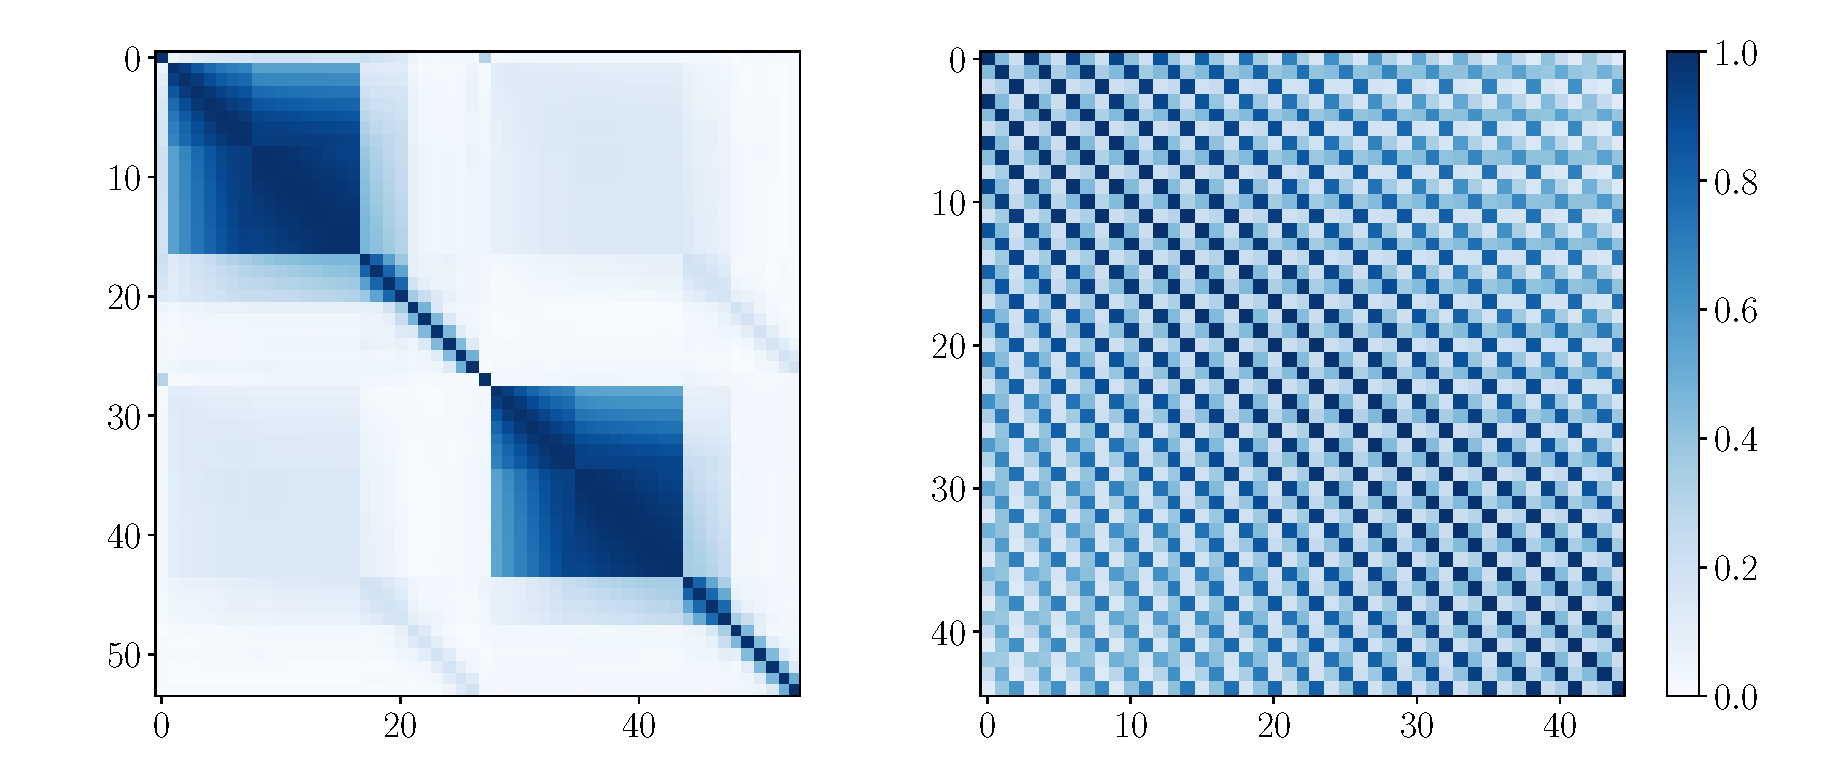
\includegraphics[width=\linewidth]{figs/ch3/corr_matrix}
	\caption{Матрицы корреляций для матрицы плана~$\bX$ и целевой матрицы~$\bY$ для данных ECoG}
	\label{ch3:fig:corr_matrix}
\end{figure}

\textbf{Результаты.}
Применим метод SymImp QPFS для различных значений коэффициента~$\alpha_3$ согласно формуле~\eqref{ch3:eq:alphas3}.
Зависимость значимостей целевых векторов~$\bz_y$ относительно коэффициента~$\alpha_3$ для различных значений~$k$ показана на Рис.~\ref{ch3:fig:features_vs_alpha_ecog}.
Значимости целевых векторов почти одинаковы для всех координат запястья при прогнозировании одного отсчёта времени ($k = 1$), 
что отражает независимость между координатами $x$, $y$ и $z$.
Для $k = 2$ и $k = 3$ значимости некоторых целевых векторов становятся нулевыми при увеличении~$\alpha_3$.
Вертикальные линии соответствуют оптимальному значению~$\alpha_3$, вычисленному по~\eqref{ch3:eq:alpha_3}. 
При этом значении $\alpha_3$ значимости компонент~$\bz_y$ совпадают. 
Таким образом, метод не учитывает различия между целевыми векторами для $k=1, 2, 3$.

\begin{figure}[ht]
	\begin{minipage}{.5\linewidth}
		\subfloat{
			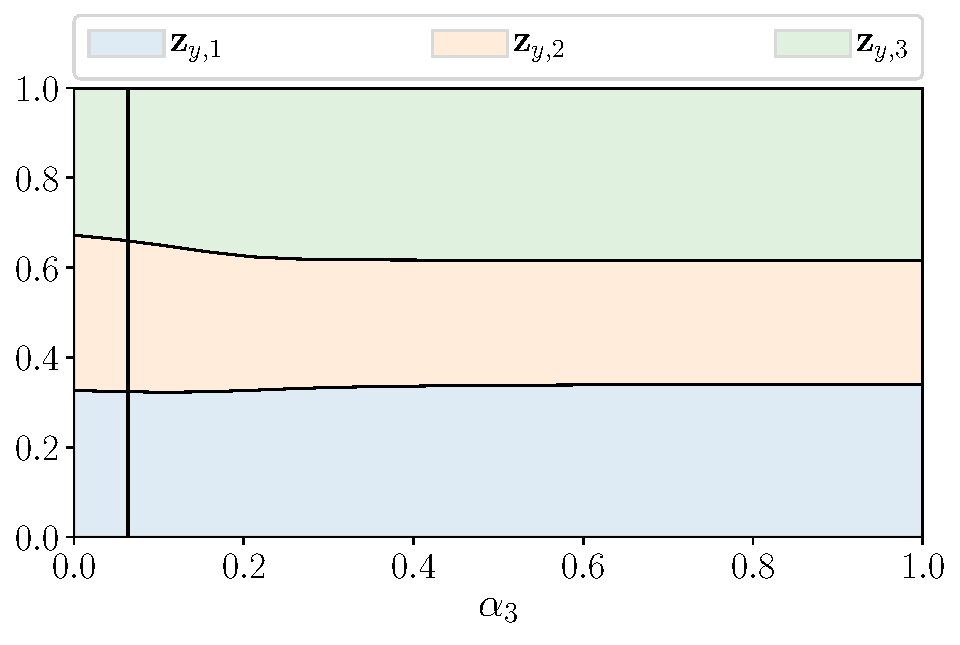
\includegraphics[width=\linewidth]{figs/ch3/features_vs_alpha_ecog_3}}
	\end{minipage}%
	\begin{minipage}{.5\linewidth}
		\subfloat{
			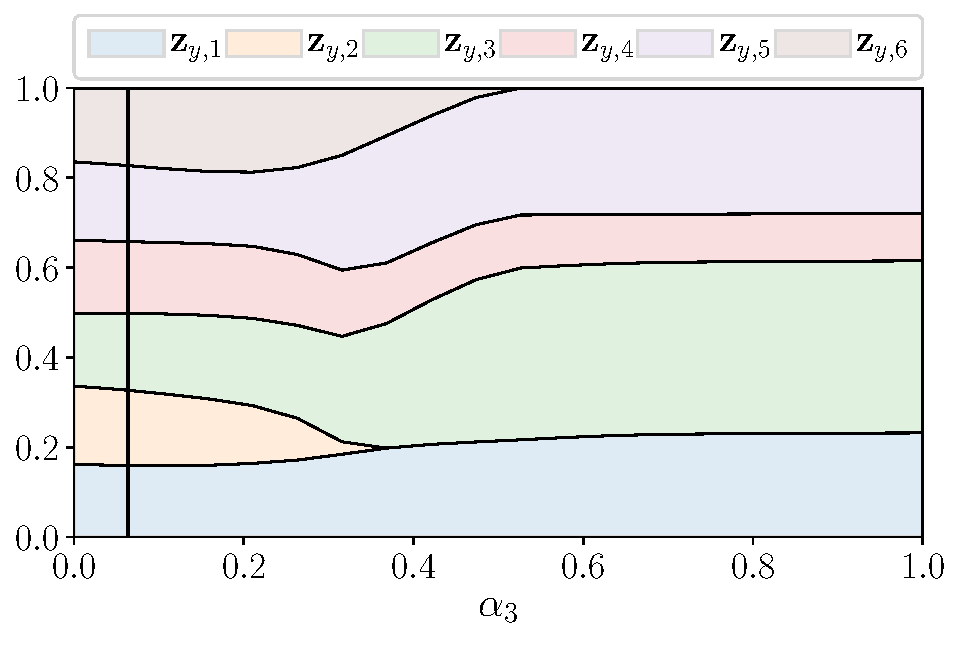
\includegraphics[width=\linewidth]{figs/ch3/features_vs_alpha_ecog_6}}
	\end{minipage}\par\medskip
	\subfloat{
		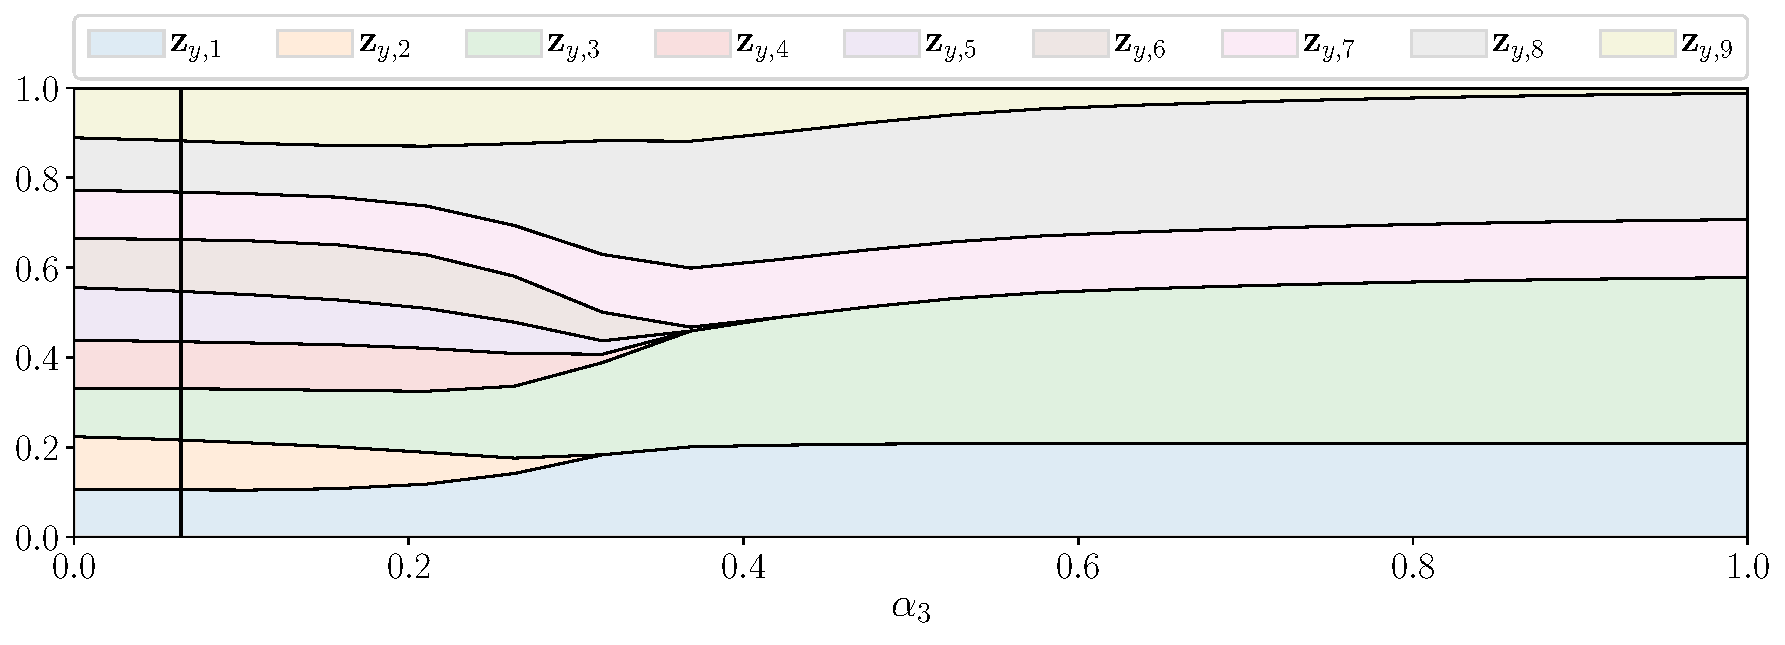
\includegraphics[width=\linewidth]{figs/ch3/features_vs_alpha_ecog_9}}
	
	\caption{Значимости целевых векторов~$\bz_y$ в зависимости от~$\alpha_3$ для метода SymImp QPFS}
	\label{ch3:fig:features_vs_alpha_ecog}
\end{figure}

Предлагаемые методы QPFS для случая векторной целевой переменной, приведенные в таблице~\ref{ch3:tbl:summary} применяются для набора данных ECoG. 
Решим задачу выбора признаков для каждого из методов, чтобы получить вектора значимостей признаков. 
Отсортируем по убыванию признаки по значению их значимостей. Обучим линейную модель, постепенно добавляя в неё признаки. 
Исследуются значения описанных критериев качества при увеличении количества отобранных признаков. 
На Рис.~\ref{ch3:fig:ecog_3_30_metrics} показаны результаты для случая прогнозирования $k = 30$ отсчётов времени. 
Порог значимости признаков~$\tau$ обозначен цветными тиками. 
Пороговые значения $\tau$ для предлагаемых методов больше, чем для базового метода RelAgg. 
Метод SymImp имеет большой порог, не позволяя получить малый набор признаков.
Однако метод SymImp обладает наилучшей предсказательной способностью с точки зрения sRMSE на тестовых данных.
Второй по качеству результат по sRMSE показал метод AsymImp.
Все предложенные методы достигают меньшей ошибки на тестовой выборке по сравнению с методом RelAgg. 
Критерий устойчивости также выше для предложенных методов.
Метод AsymImp показывает лучшие результаты с точки зрения качества прогнозирования и размера выбранного подмножества признаков.

\begin{figure}[ht]
	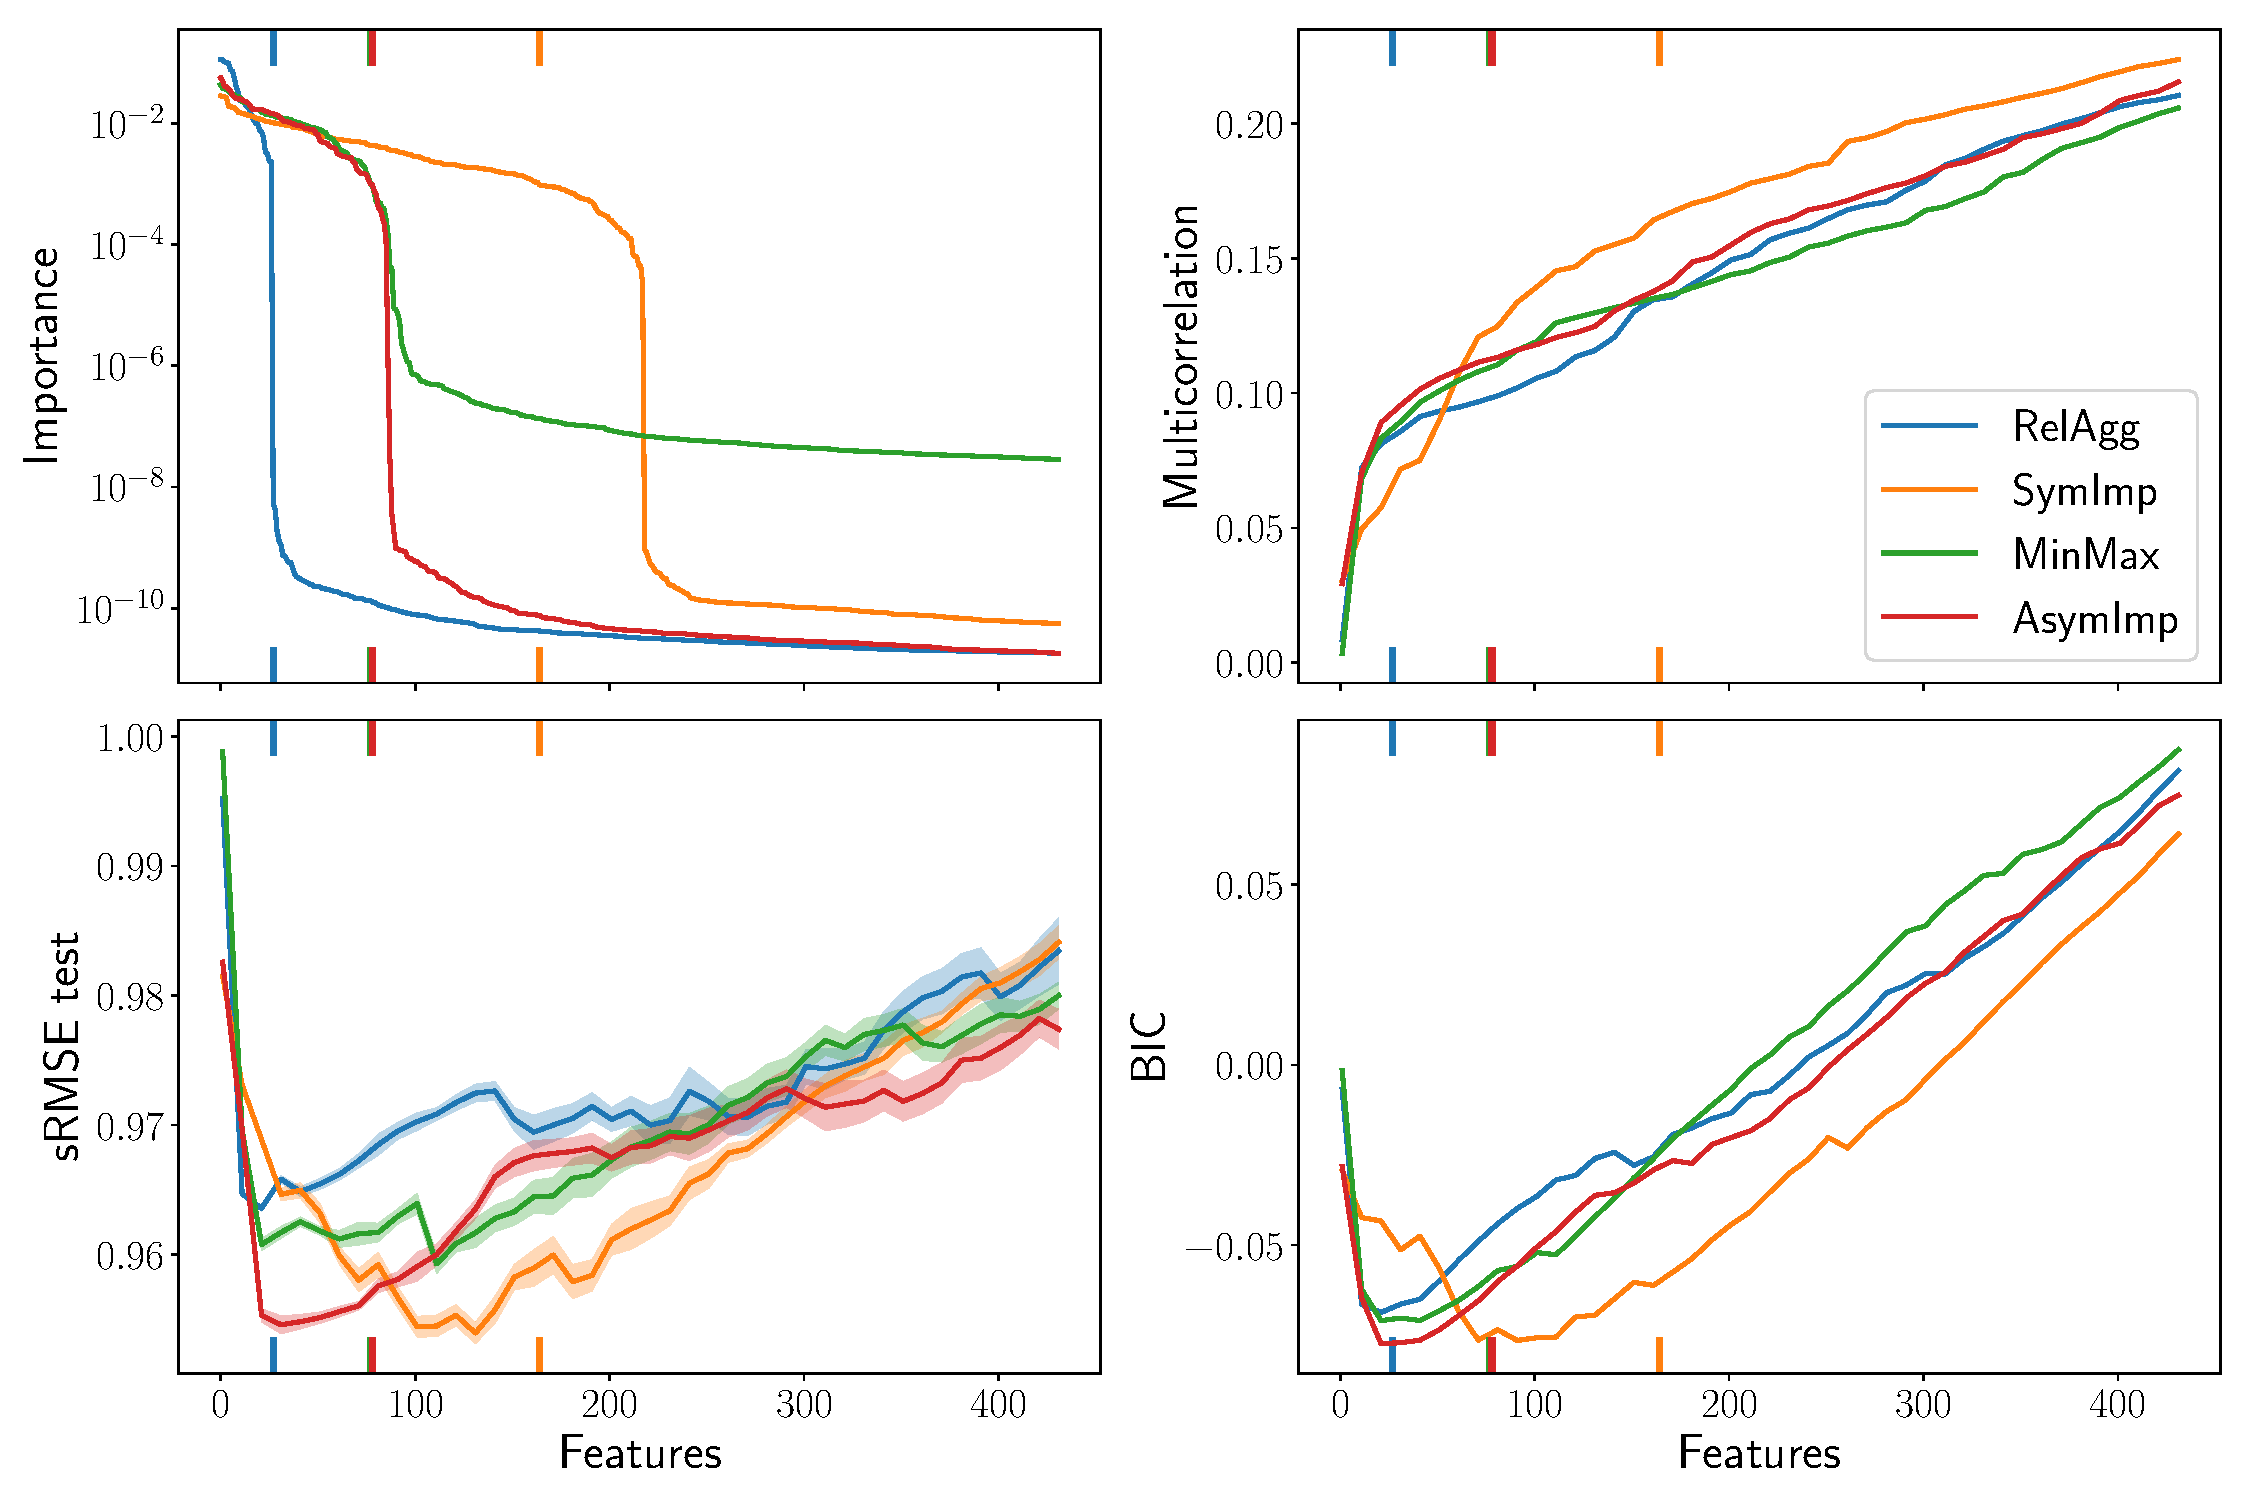
\includegraphics[width=\linewidth]{figs/ch3/ecog_3_30_metrics}
	\caption{Сравнение предложенных методов выбора признаков для данных ECoG при прогнозировании $k = 30$ отсчётов времени}
	\label{ch3:fig:ecog_3_30_metrics}
\end{figure}

Чтобы сравнить структуру выбранных подмножеств признаков и исследовать стабильность процедуры выбора признаков, используется метод генерации данных с помощью бутстрепа. 
Генерируется множество подвыборок, выбирая объекты по одному с возвращениями. 
Затем решается задача выбора признаков для каждой пары матрицы исходных объектов~$\bX$ и  матрицы целевых объектов~$\bY$.
Сравниваются полученные вектора значимостей для различных подвыборок данных. 
В качестве меры стабильности работы методов вычисляется средний попарный коэффициент корреляции Спирмена и попарное $\ell_2$ расстояние.
В таблице~\ref{ch3:tbl:stability} показана средняя ошибка sRMSE, размер подмножества признаков и описанные статистики для каждого метода. 
Ошибка считалась на обученной линейной модели с использованием $50$ признаков с наибольшими значениями значимостей.
Asymimp дает наименьшую ошибку на тестовой выборке. 
Размер выбранных подмножеств объектов завышен при использовании порогового значения~$\tau=10^{-4}$. 
Оптимальное значение~$\tau$ может быть подобрано с помощью процедуры кросс-валидации.

\begin{table}[ht]
	\caption{Стабильность предложенных методов выбора признаков}
	\centering
	\begin{tabular}{l|ccccc}
		\hline
		& sRMSE  & $\|\ba\|_0$ & Spearman $\rho$ & $\ell_2$ \\ \hline
		RelAgg & 0.965 $\pm$ 0.002 & 26.8 $\pm$ 3.8 & 0.915 $\pm$ 0.016 & 0.145 $\pm$ 0.018   \\
		SymImp & 0.961 $\pm$ 0.001 & 224.4 $\pm$ 9.0 & 0.910 $\pm$ 0.017 & 0.025 $\pm$ 0.002   \\
		MinMax & 0.961 $\pm$ 0.002 & 101.0 $\pm$ 2.1& 0.932 $\pm$ 0.009 & 0.059 $\pm$ 0.004   \\
		AsymImp & 0.955 $\pm$ 0.001 & 85.8 $\pm$ 10.2& 0.926 $\pm$ 0.011 & 0.078 $\pm$ 0.007  \\ \hline
	\end{tabular}
	\label{ch3:tbl:stability}
\end{table}

Для того, чтобы сравнить методы снижения размерности и выбора признаков, используется модель PLS, описанная в главе~\ref{ch:pls}. 
На Рис.~\ref{ch3:fig:pls_vs_k} показана ошибка sRMSE на тренировочной и тестовой выборках в зависимости от размерности скрытого пространства~$l$.
Ошибка на тестовой выборке достигает минимума при $l = 11$.
Метод PLS является более гибким подходом по сравнению с линейной моделью, построенной на подмножестве признаков, так как использует все исходные признаки.
Это приводит к меньшей ошибке, но модель не является разреженной.

На Рис.~\ref{ch3:fig:models} приведено сравнение 3 моделей: линейной регрессии; регрессии PLS, построенной на 100 признаках QPFS; регрессии PLS со всеми признаками.
Линейная регрессия со всеми признаками не рассматривается, так как ее результаты близки к константному прогнозу. На рисунке также приведены результаты методов lasso и elastic net, которые широко используются для выбора признаков.
В данном эксперименте использовался метод Asymimp QPFS.
Размерность скрытого пространства PLS $l = 15$.
Результаты регрессии PLS значительно лучше, линейной регрессии с признаками QPFS.
Это означает, что последняя модель не является достаточно гибкой.
Тем не менее, лучший результат показывает модель PLS, построенная на признаках QPFS. 
Данная модель является разреженной, так как использует только 100 исходных признаков.
Способность модели PLS находить оптимальное скрытое представление данных улучшает предсказательную способность модели.

\begin{figure}[ht]
	\begin{minipage}{.41\linewidth}
		\centering
		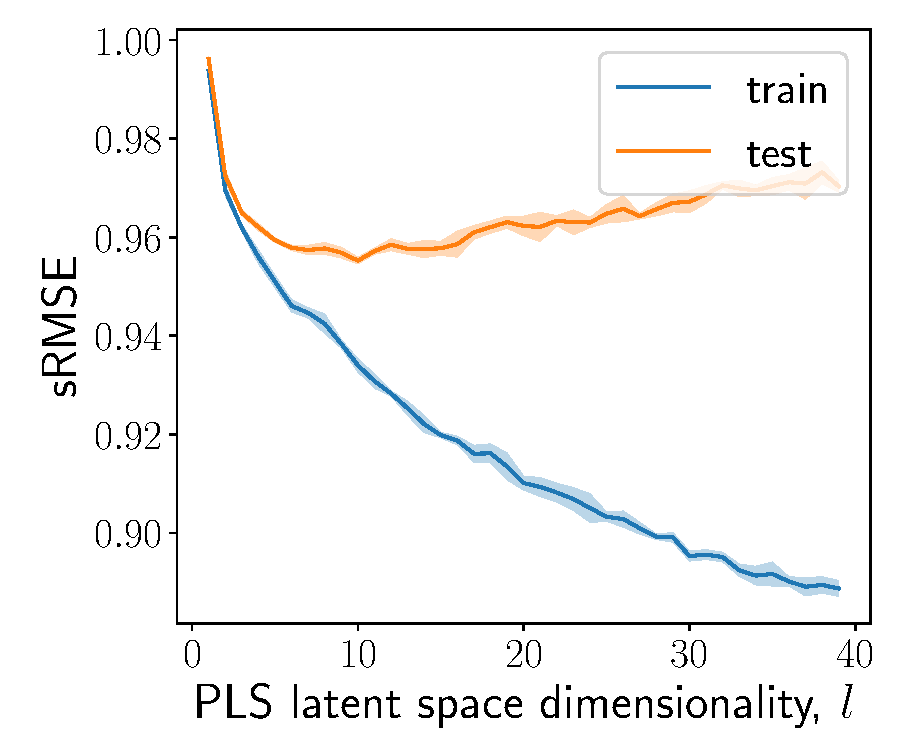
\includegraphics[width=1.\linewidth]{figs/ch3/pls_vs_k}
		\caption{ Ошибка sRMSE на тестовой выборке для модели PLS}
		\label{ch3:fig:pls_vs_k}
	\end{minipage}%
	\begin{minipage}{.55\linewidth}
		\centering
		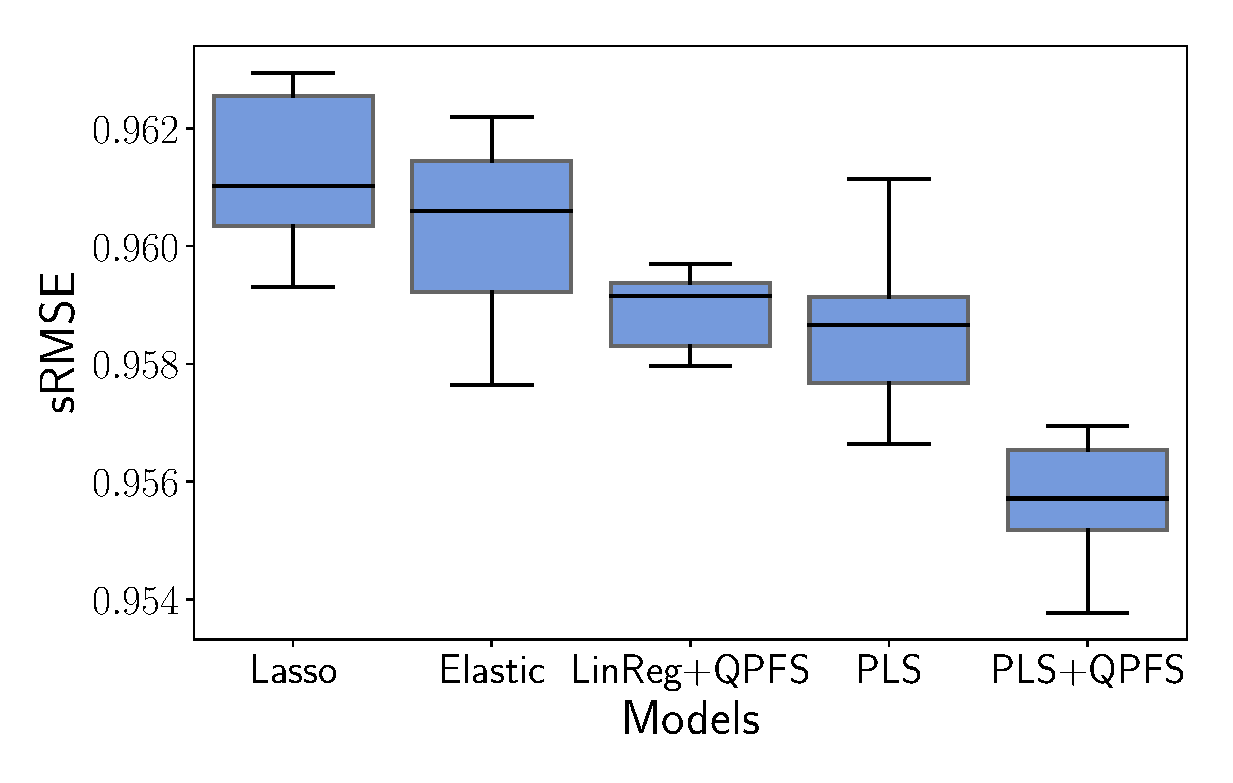
\includegraphics[width=1.\linewidth]{figs/ch3/models2}
		\caption{Диаграммы размаха значений sRMSE на тестовой выборке для моделей Lasso, Elastic, LinReg+QPFS, PLS, PLS+QPFS}
		\label{ch3:fig:models}
	\end{minipage}
\end{figure}


\newpage{}
\chapter{Выбор параметров нелинейных моделей с помощью квадратичного отбора признаков}
\label{ch:newton_qpfs}

Функция ошибки для моделей с большим числом параметров имеет сложный ландшафт с многими локальными минимумами.
В этом случае алгоритм оптимизации приводит к разным решениям в зависимости от инициализации исходных параметров.

Алгоритм оптимизации представляет собой итерационный процесс.
На каждом шаге для получения следующего приближения параметров модели обновляются текущие параметры.
Разработано множество алгоритмов оптимизации первого порядка, использующих вектор первых производных функции ошибки.
Наиболее известными алгоритмами являются градиентный спуск, 
метод момента Нестерова~\cite{nesterov1983momentum}, AdaGrad~\cite{duchi2011adagrad}, Adam~\cite{kingma2014adam}.
Данные алгоритмы используются для оптимизации глубоких нейронных сетей~\cite{goodfellow2016deeplearningbook}.
Метод Ньютона~--- алгоритм второго порядка, использующий матрицу вторых производных функции ошибки.
Метод Ньютона находит обновления параметров для квадратичной аппроксимации функции ошибки и сходится за адекватное число итераций.
Недостатком методов оптимизации второго порядка является огромная и плохо обусловленная матрица Гессиана.
Процесс оптимизации в этом случае расходится и является вычислительно дорогостоящим.
Авторы~\cite{avriel2003nonlinear,blaschke1997convergence} предлагают аппроксимации для матрицы Гессиана и регуляризацию для решения этой проблемы.
В статье~\cite{botev2017newtondeeplearning} метод Ньютона применяется к глубоким нейронным сетям.

В данной главе приводится анализ параметров модели, которые не находятся в оптимуме.
Приводится метод выбора активных параметров модели, основанный на методе QPFS, который подробно описан в главе~\ref{ch:qpfs}.
Рассматриваются задачи нелинейной регрессии с квадратичной функцией потерь, логистической регрессии с кросс-энтропийной функцией потерь.  

%%%%%%%%%%%%%%%%%%%%%%%%%%%%%%%%%%%%%%%%%%%%%%%%
\section{Задача выбора параметров для оптимизации нелинейных моделей}
\label{sec:ch4:newton_qpfs_param_selection}
%%%%%%%%%%%%%%%%%%%%%%%%%%%%%%%%%%%%%%%%%%%%%%%%

Модель $f( \bx, \btheta)$ с параметрами $\btheta \in \mathbb{R}^p$ предсказывает целевую переменную~$y \in \bbY$ по исходной переменной~$\bx \in \bbR^{n}$. Пространство~$\bbY$ представляет собой бинарные метки классов~$\{0, 1\}$ для задачи двухклассовой классификации и~$\bbR$ для задачи регрессии.
Даны исходная матрица~$\bX = [\bx_1, \dots, \bx_m]^{\T} \in \bbR^{m \times n}$ и целевой столбец~$\by = [y_1, \dots, y_m]^{\T} \in \bbY^{m}$. 
Цель состоит в нахождении оптимальных параметров~$\btheta^*$.
Параметры~$\btheta$ вычисляются минимизацией функции ошибки:
\begin{equation}
	\btheta^* = \argmin_{\btheta \in \bbR^p} \cL(\btheta, \bX, \by).
	\label{ch4:eq:error_function}
\end{equation}
Данная задача полностью соответствует рассмотренной задаче~\eqref{ch1:eq:loss_min_param} для случая скалярной целевой переменной ($r=1$).
В качестве функции ошибки~$\cL (\btheta, \bX, \by)$ рассматриваются квадратичная ошибка для задачи регрессии:
\begin{equation}
	\cL(\btheta, \bX, \by) = \frac 12 \| \by - \mathbf{f}(\bX, \btheta) \|^2 = \frac 12 \sum_{i=1}^m \bigl( y_i - f(\bx_i,  \btheta)\bigr)^2,
	\label{ch4:eq:squared_error}
\end{equation}
и функция кросс-энтропии для задачи бинарной классификации: 
\begin{equation}
	\cL(\btheta, \bX, \by) = \sum_{i=1}^m \bigl[y_i \log f (\bx_i , \btheta) + (1-y_i) \log \bigl(1 - f (\bx_i , \btheta)\bigr)\bigr].
	\label{ch4:eq:log_loss}
\end{equation}

Задача~\eqref{ch4:eq:error_function} решается с помощью итеративной процедуры оптимизации. 
Для получения параметров на шаге~$k$ текущие параметры $\btheta^{k-1}$ обновляются по следующему правилу:
\begin{equation}
	\btheta^k = \btheta^{k - 1} + \Delta \btheta^{k - 1}.
	\label{ch4:eq:update_rule}
\end{equation}
Для выбора вектора обновлений~$\Delta \btheta$ используется метод оптимизации Ньютона.

Метод Ньютона нестабилен и вычислительно сложен. 
В работе предлагается стабильный метод Ньютона. 
Перед шагом градиента предлагается выбрать подмножество активных параметров модели, которые оказывают наибольшее влияние на функцию ошибки~$\cL (\btheta, \bX, \by)$.
Введём определение активного параметра модели, используя необходимое условие оптимальности первого порядка.
\begin{definition}
	\label{ch4:def:active_param}
	Параметр $\theta_j$ для модели $f(\bx, \btheta)$ является \textit{активным}, если $\bJ^{\T} (\mathbf{f}(\bx, \btheta) - \by) \neq 0$.
\end{definition}
Подробный вывод условия из определения приводится в разделе~\ref{sec:ch4:newton_qpfs_algorithm}.
Обновление параметров производится только для отобранного множества индексов~$\cA = \bigl\{j: a_j = 1, \ba \in \{0, 1\}^p\bigr\}$
\begin{align*}
	\btheta_{\cA}^k &= \btheta_{\cA}^{k - 1} + \Delta \btheta_{\cA}^{k - 1}, \quad \btheta_{\cA} = \{\theta_j: j \in \cA \}, \\
	\btheta_{\bar{\cA}}^k &= \btheta_{\bar{\cA}}^{k - 1}, \quad \btheta_{\bar{\cA}} = \{\theta_j: j \notin \cA \}.
\end{align*}
Чтобы выбрать оптимальное подмножество индексов~$\cA$, из всех возможных $2^p - 1$~подмножеств, вводится функция ошибки
\begin{equation}
	\ba = \argmin_{\ba' \in \{0, 1\}^p} S(\ba', \bX, \by, \btheta),
	\label{ch4:eq:subset_selection}
\end{equation}
аналогичная функции ошибки~\eqref{ch3:eq:feature_selection} для задачи выбора признаков. 
Задача~\eqref{ch4:eq:subset_selection} решается на каждом шаге $k$ процесса оптимизации для текущих параметров~$\btheta^k$.

Метод QPFS используется для решения задачи~\eqref{ch4:eq:subset_selection}.
QPFS выбирает подмножество параметров~$\ba$ для вектора обновлений~$ \Delta \btheta$, которые оказывают наибольшее влияние на вектор остатков и являются попарно независимыми.
Функция ошибки~\eqref{ch3:eq:qpfs_problem} соответствует функции ошибки~$S(\ba, \bX, \by, \btheta)$
\begin{equation}
	\ba = \argmax_{\ba' \in \{1, 0\}^p} S(\ba', \bX, \by, \btheta) \Leftrightarrow \argmin_{\ba  \in \bbR^p_+, \, \|\ba\|_1=1} \bigl[\ba^{\T} \bQ \ba - \alpha \cdot \mathbf{b}^{\T} \ba \bigr].
\end{equation}
В работе показано, что для модели нелинейной регрессии с квадратичной функцией ошибки~\eqref{ch4:eq:squared_error} и для модели логистической регрессии с кросс-энтропией~\eqref{ch4:eq:log_loss}, каждый шаг оптимизации эквивалентен задаче линейной регрессии~\eqref{ch3:eq:linear_regression}.

%%%%%%%%%%%%%%%%%%%%%%%%%%%%%%%%%%%%%%%%%%%%%%%%
\section{Метод Ньютона для оптимизации параметров}
\label{sec:ch4:newton_algorithm}
%%%%%%%%%%%%%%%%%%%%%%%%%%%%%%%%%%%%%%%%%%%%%%%%

Метод Ньютона использует условие оптимизации первого порядка для задачи~\eqref{ch4:eq:error_function} и линеаризует градиент $S (\btheta)$:
\[
	\nabla S (\btheta + \Delta \btheta) = \nabla S(\btheta) + \bH \cdot \Delta \btheta = \bZero,
\]
\[
	\Delta \btheta = - \bH^{-1} \nabla S(\btheta).
\]
где $\bH = \nabla^2 S(\btheta)$ является матрицей Гессиана функции ошибки $S(\btheta)$.

Итерация~\eqref{ch4:eq:update_rule} метода Ньютона имеет вид
\begin{equation}
	\btheta^k = \btheta^{k-1} - \bH^{-1} \nabla S(\btheta).
	\label{ch4:eq:newton_step}
\end{equation}
На каждой итерации требуется обращать матрицу Гессиана $\bH$.
Мерой плохой обусловленности для матрицы Гессиана~$\bH$ является число обусловленности
\[
	\kappa(\bH) = \frac{\lambda_{\text{max}}(\bH)}{\lambda_{\text{min}}(\bH)},
\]
где $\lambda_{\text{max}}(\bH), \lambda_{\text{min}}(\bH)$ являются максимальным и минимальным собственными значениями~$\bH$. Большое число обусловленности~$\kappa (\bH)$ приводит к нестабильности процесса оптимизации.
Предложенный метод уменьшает размер матрицы Гессиана~$\bH$. Согласно экспериментам, приведенным в разделе~\ref{sec:ch4:newton_qpfs_exp} предлагаемый метод приводит к меньшему числу обусловленности~$\kappa (\bH)$.

Размер шага метода Ньютона может быть чрезмерно большим. Для контроля размера шага обновлений добавим параметр $\eta$ в правило обновления~\eqref{ch4:eq:update_rule}
\[
	\btheta^k = \btheta^{k - 1} + \eta \Delta \btheta^{k - 1}, \quad \eta \in [0, 1].
\]

Для выбора соответствующего размера шага~$\eta$ используется правило Армихо~\cite{armijo1966minimization}. Выбирается максимальное~$\eta$ так, чтобы выполнялось условие
\[
	S(\btheta^{k - 1} + \eta \Delta \btheta^{k - 1}) < S(\btheta^{k - 1}) + \gamma \eta \nabla S^{\T}(\btheta^{k-1})\btheta^{k - 1}, \quad \gamma \in [0, 0.5].
\]

\begin{theorem}
	Пусть модель $f (\bx , \btheta)$ близка к линейной в окрестности точки $\btheta + \Delta \btheta$
	\begin{equation}
		\mathbf{f}(\bX , \btheta + \Delta \btheta) \approx \mathbf{f}(\bX , \btheta) + \bJ \cdot \Delta  \btheta,
		\label{ch4:eq:linearization}
	\end{equation}
	где $\mathbf{J} \in \bbR^{m \times p}$ является матрицей Якоби
	\begin{equation*}
		\bJ = 
		\begin{pmatrix}
			\frac{\partial f(\bx_1 , \btheta)}{\partial \theta_1} & \dots & 
			\frac{\partial f(\bx_1 , \btheta)}{\partial \theta_p} \\
			\dots & \dots & \dots \\
			\frac{\partial f(\bx_m , \btheta)}{\partial \theta_1} & \dots & 
			\frac{\partial f(\bx_m , \btheta)}{\partial \theta_p}
		\end{pmatrix}.
	\end{equation*}
	Тогда вектор обновления~$\Delta \btheta$ для функции ошибки~\eqref{ch4:eq:squared_error} является решением задачи линейной регрессии
	\begin{equation}
		\| \be - \bF \Delta \btheta \|_2^2 \rightarrow \min_{\Delta \btheta \in \bbR^{p}},
		\label{ch4:eq:lin_reg_nonlin_reg}
	\end{equation}
	где $\be = \mathbf{f} - \by$ и $\bF = \bJ$.
\end{theorem}
\begin{proof}
	В соответствии предположением~\eqref{ch4:eq:linearization} градиент~$\nabla S(\btheta)$ и матрица Гессиана~$\bH$ имеют вид
	\begin{equation}
		\nabla S(\btheta) = \bJ^{\T} (\by - \mathbf{f}), \quad \bH = \bJ^{\T} \bJ.
		\label{ch4:eq:nonlin_reg_deriv}
	\end{equation}
	Тогда шаг метода Ньютона~\eqref{ch4:eq:newton_step} и правило обновления~\eqref{ch4:eq:update_rule} принимают вид
	\[
		\btheta^k = \btheta^{k - 1} + \Delta \btheta^{k - 1} = \btheta^{k - 1} + (\bJ^{\T} \bJ)^{-1}\bJ^{\T}(\mathbf{f} - \by).
	\]
	Таким образом, согласно теореме Гаусса-Маркова, вектор обновления~$\Delta \btheta$ является решением задачи регрессии~\eqref{ch4:eq:lin_reg_nonlin_reg}.
\end{proof}
В качестве нелинейной модели рассматривается модель двухслойной нейронной сети. В этом случае модель~$f (\bx, \btheta)$ принимает вид:
\[
	f(\bx, \btheta) = \sigma(\bx^{\T} \bW_1) \bw_2.
\]
Здесь~$\bW_1 \in \bbR^{m \times h}$~--- матрица параметров, которые соединяют исходные признаки с $h$ скрытыми нейронами. Функция нелинейности $\sigma(\cdot)$ применяется поэлементно. Параметры~$\bw_2 \in \bbR^{h \times 1}$ соединяют скрытые нейроны с выходом. 
Вектор параметров модели~$\btheta$ представляет собой объединение векторизованных матриц~$\bW_1$, $\bw_2$.

\begin{theorem}
Рассмотрим модель логистической регрессии вида $f(\bx , \btheta) = \sigma(\bx^{\T} \btheta)$ с сигмоидной функцией активации~$\sigma(\cdot)$. 
Вектор обновлений $\Delta \btheta$ для функции ошибки~\eqref{ch4:eq:log_loss} является решением задачи линейной регрессии
\begin{equation}
	\| \be - \bF \Delta \btheta \|_2^2 \rightarrow \min_{\Delta \btheta \in \bbR^{p}},
	\label{ch4:eq:lin_reg_log_reg}
\end{equation}
где $\be = \bR^{-1/2} (\by - \mathbf{f})$ и $\bF = \bR^{1/2}\bX$.
\end{theorem}
\begin{proof}
	Градиент и Гессиан функции ошибки~\eqref{ch4:eq:log_loss} равны
	\begin{equation}
		\nabla S(\btheta) = \bX^{\T} (\mathbf{f} - \by), \quad \bH = \bX^{\T} \bR \bX,
		\label{ch4:eq:log_reg_deriv}
	\end{equation}
	где $\bR$~--- это диагональная матрица с диагональными элементами $f(\bx_i , \btheta) \cdot (1 - f(\bx_i , \btheta))$.
	
	Правило обновления~\eqref{ch4:eq:update_rule} в этом случае принимает вид
	\[
		\btheta^k = \btheta^{k - 1} + (\bX^{\T} \bR \bX)^{-1} \bX^{\T} (\by - \mathbf{f}).
	\]
	Таким образом, согласно теореме Гаусса-Маркова, вектор обновления~$\Delta \btheta$ является решением задачи регрессии~\eqref{ch4:eq:lin_reg_nonlin_reg}.
\end{proof}
Данный алгоритм известен как итеративный алгоритм взвешенных наименьших квадратов (IRLS)~\cite{holland1977robust}. 

%%%%%%%%%%%%%%%%%%%%%%%%%%%%%%%%%%%%%%%%%%%%%%%%
\section{Метод Ньютона с выбором параметров с помощью квадратичного программирования}
\label{sec:ch4:newton_qpfs_algorithm}
%%%%%%%%%%%%%%%%%%%%%%%%%%%%%%%%%%%%%%%%%%%%%%%%

Предлагается адаптация метода QPFS для решения задач~\eqref{ch4:eq:lin_reg_nonlin_reg} и \eqref{ch4:eq:lin_reg_log_reg}. 
Матрица парных взаимодействий~$\bQ$ и вектор релевантностей~$\bb$ имеют вид
\[
	\bQ = \text{Sim} (\bF), \quad \bb = \text{Rel} (\bF, \be).
\]

\begin{statement}
	В оптимальной точке~$\btheta^*$ вектор релевантностей~$\bb = \text{Rel} (\bF, \be)$ равен нулю.
\end{statement}
\begin{proof}
	Выборочный коэффициент корреляции равен нулю для ортогональных векторов.
	Покажем, что в оптимальной точке~$\btheta^*$ вектор~$\be$ ортогонален столбцам матрицы~$\bF$. 
	Условие оптимальности первого порядка гарантирует это свойство для модели нелинейной регрессии
	\[
		\bF^{\T} \be = \bJ^{\T} (\mathbf{f} - \by) = - \nabla S(\btheta^*) = \boldsymbol{0},
	\]
	и для модели логистической регрессии
	\[
		\bF^{\T} \be = \bX \bR^{-1/2} \bR^{1/2} (\by - \mathbf{f}) = \bX^{\T} (\by - \mathbf{f}) = \nabla S(\btheta^*) = \boldsymbol{0}.
	\]
\end{proof}
Данное утверждение используется в качестве индикатора активности параметра модели в определении~\ref{ch4:def:active_param}.
Псевдокод предлагаемого алгоритма приведён в алгоритме~\ref{ch4:alg:QPFSNewton}.

\begin{algorithm}[ht]
	\caption{QPFS + Ньютон алгоритм}
	\label{ch4:alg:QPFSNewton}
	\begin{algorithmic}
		\REQUIRE $\varepsilon$~--- допустимое отклонение;\\
		\hspace{1.07cm}$\tau$~-- пороговое значение;\\
		\hspace{1.07cm}$\gamma$~--- параметр правила Армихо.
		\ENSURE $\btheta^*$;
		\STATE  инициализировать $\btheta^0$;
		\STATE $k := 1$;
		\REPEAT
		\STATE вычислить $\be$ и $\bF$ для~\eqref{ch4:eq:lin_reg_nonlin_reg} или~\eqref{ch4:eq:lin_reg_log_reg} ;
		\vspace{0.1cm}
		\STATE $\bQ := \text{Sim} (\bF)$, $\bb := \text{Rel}(\bF, \be)$, $\alpha = \frac{\overline{\bQ}}{\overline{\bQ} + \overline{\bb}}$;
		\vspace{0.1cm}
		\STATE $\ba := \argmin_{\ba \geq 0, \, \|\ba\|_1=1}\ba^{\T} \bQ \ba - \alpha \cdot \mathbf{b}^{\T} \ba$;
		\vspace{0.1cm}
		\STATE $\cA := \{j: a_j = 1\}$;
		\vspace{0.1cm}
		\STATE вычислить $\nabla S(\btheta^{k-1})$, $\bH$ для \eqref{ch4:eq:nonlin_reg_deriv} или \eqref{ch4:eq:log_reg_deriv};
		\vspace{0.1cm}
		\STATE $\Delta \btheta^{k-1} = - \bH^{-1} \nabla S(\btheta^{k-1})$;
		\vspace{0.1cm}
		\STATE $\eta := \text{ArmijoRule}(\btheta^{k-1}, \gamma)$;
		\vspace{0.1cm}
		\STATE $\btheta_{\cA}^k = \btheta_{\cA}^{k - 1} + \eta \Delta \btheta_{\cA}^{k - 1}$;
		\vspace{0.1cm}
		\STATE $k := k + 1$;
		\vspace{0.1cm}
		\UNTIL{$\frac{\| \btheta^k - \btheta^{k-1} \|}{\| \btheta^k \|} < \varepsilon$}
	\end{algorithmic}
\end{algorithm}

%%%%%%%%%%%%%%%%%%%%%%%%%%%%%%%%%%%%%%%%%%%%%%%%
\section{Анализ значимостей параметров нелинейных моделей}
\label{sec:ch4:newton_qpfs_exp}
%%%%%%%%%%%%%%%%%%%%%%%%%%%%%%%%%%%%%%%%%%%%%%%%

Целью вычислительного эксперимента является исследование свойств предложенного метода и сравнение его с другими методами. 

Исследована зависимость параметров метода QPFS для задачи нелинейной регрессии~\eqref{ch4:eq:lin_reg_nonlin_reg} и задачи логистической регрессии~\eqref{ch4:eq:lin_reg_log_reg}. 
Предположим, что вектор параметров~$\btheta^0$ лежит вблизи оптимального вектора параметров~$\btheta^*$. 
Рассмотрим отрезок
\[
	\btheta_{\beta} = \beta \btheta^* + (1 - \beta) \btheta^0; \quad \beta \in [0, 1] .
\]

Сгенерируем синтетический набор данных с 300 объектами и 7 признаками для задачи логистической регрессии. 
Ландшафт функции ошибки~\eqref{ch4:eq:log_loss} на сетке двух случайно выбранных параметров показан на Рис.~\ref{ch4:fig:log_reg_error}.
Поверхность функции ошибки выпуклая с вытянутыми линиями уровня вдоль некоторых параметров модели.
Добавим случайный шум к оптимальным параметрам~$\btheta^*$, чтобы получить точку~$\btheta^0$. Поведение вектора~$\bb$ на отрезке между~$\btheta^0$ и~$\btheta^*$ показано на Рис.~\ref{ch4:fig:log_reg_b_wrt_beta}.
Компоненты~$\bb$ начинают резко уменьшаться по мере приближения к оптимальной точке $\btheta^*$.
\begin{figure}[h]
	\centering
	\begin{minipage}{.47\textwidth}
		\centering
		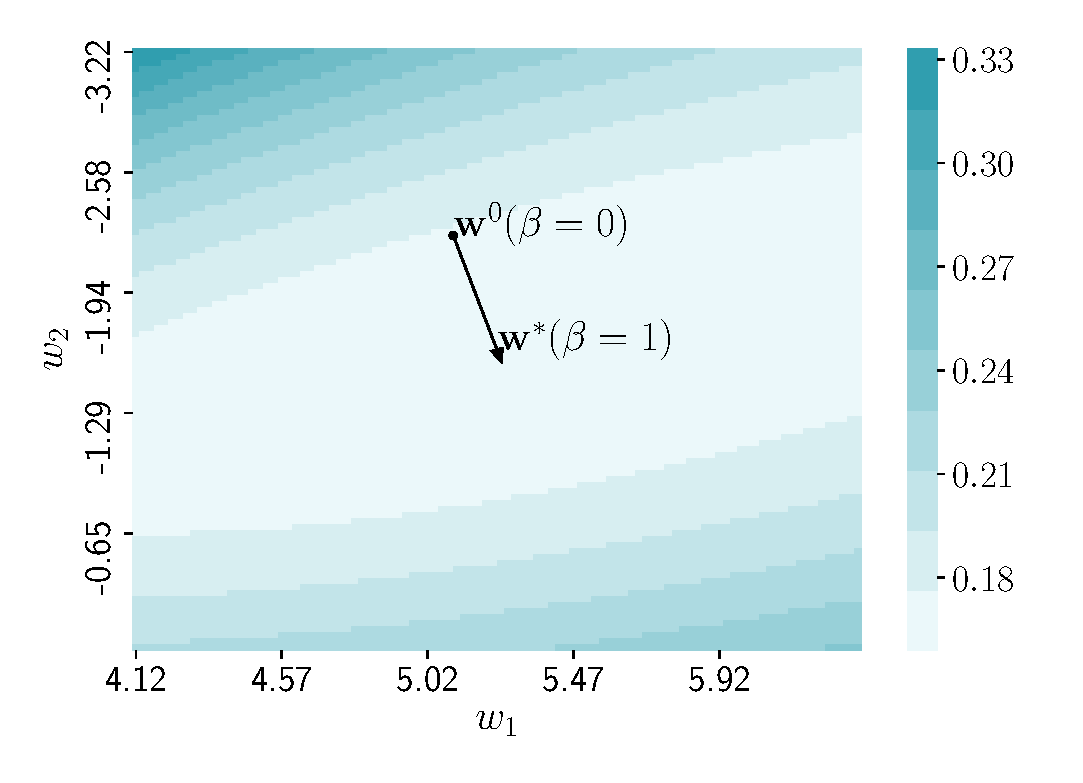
\includegraphics[width=\linewidth]{figs/ch4/log_reg_error}
		\caption{Поверхность функции ошибки для логистической регрессии}
		\label{ch4:fig:log_reg_error}
	\end{minipage}%
	\begin{minipage}{.47\textwidth}
		\centering
		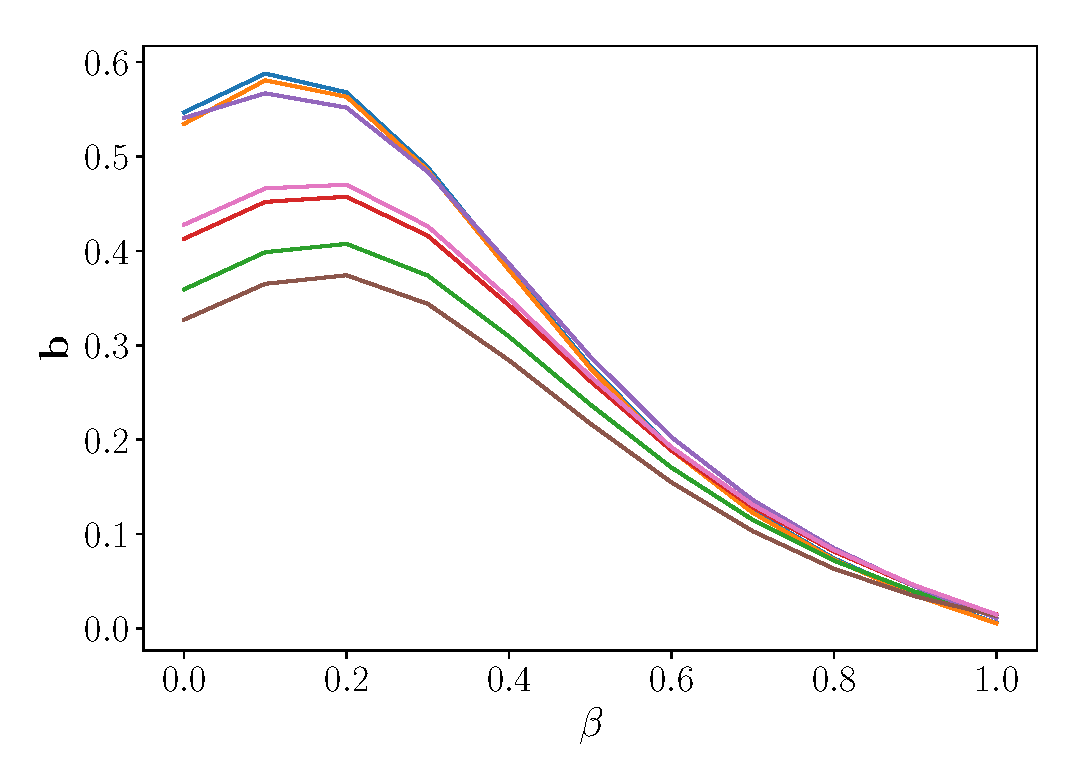
\includegraphics[width=\linewidth]{figs/ch4/log_reg_b_wrt_beta}
		\caption{Релевантность параметров для логистической регрессии}
		\label{ch4:fig:log_reg_b_wrt_beta}
	\end{minipage}
\end{figure}

Для модели нелинейной регрессии используется классический набор данных Boston Housing с 506 объектами и 13 признаками.
Для простоты нейронная сеть содержит два скрытых нейрона.
Ландшафт функции ошибок для модели нейронной сети является более сложным. 
Функция ошибки не является выпуклой и содержит множество локальных минимумов.
Двумерный ландшафт функции ошибок для этого набора данных показан на Рис.~\ref{ch4:fig:neural_error}. 
Сетка строится для двух случайных параметров из матрицы~$\bW_1$.
Аналогично на Рис.~\ref{ch4:fig:neural_b_wrt_beta} показано, как изменяется вектор~$\bb$ при движении от точки~$\btheta^0$ до точки~$\btheta^*$. 
Компоненты вектора $\bb$ становятся близки к нулю вблизи оптимума. 
При достижении оптимального значения различные параметры влияют на остатки модели~$\be$.
\begin{figure}[h]
	\centering
	\begin{minipage}{.5\textwidth}
		\centering
		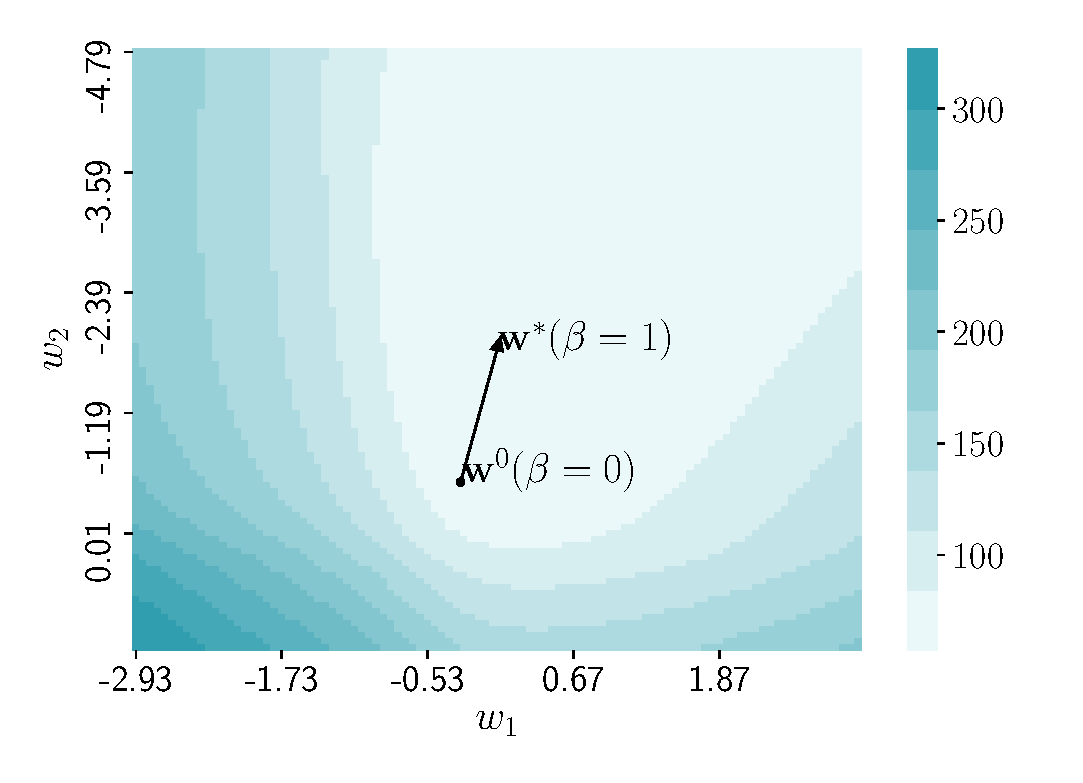
\includegraphics[width=\linewidth]{figs/ch4/neural_error}
		\caption{Поверхность функции ошибки для нейронной сети}
		\label{ch4:fig:neural_error}
	\end{minipage}%
	\begin{minipage}{.5\textwidth}
		\centering
		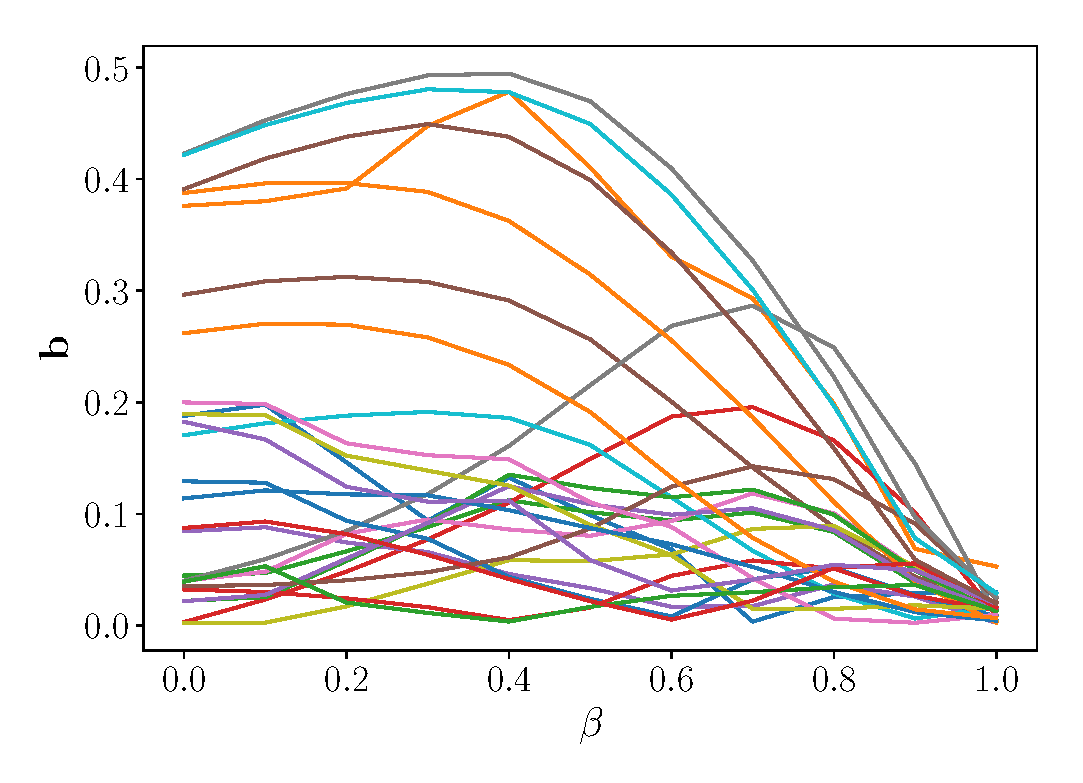
\includegraphics[width=\linewidth]{figs/ch4/neural_b_wrt_beta}
		\caption{Релевантность параметров первого слоя для модели нейронной сети}
		\label{ch4:fig:neural_b_wrt_beta}
	\end{minipage}
\end{figure}

На Рис.~\ref{ch4:fig:irls_qpfs_2d} показан процесс оптимизации для предложенного метода в случае логистической регрессии с двумя параметрами модели. 
Даже для двумерной задачи решение метода Ньютона нестабильно и число обусловленности $\kappa(\bH)$ матрицы Гессиана~$\bH$ может быть чрезвычайно большим. 
На каждом шаге алгоритма метод QPFS выбирает активные параметры для оптимизации. 
В данном примере предложенный метод выбирает и обновляет только один параметр на каждой итерации на первых шагах. 
Это делает метод более устойчивым.

\begin{figure}
	\centering
	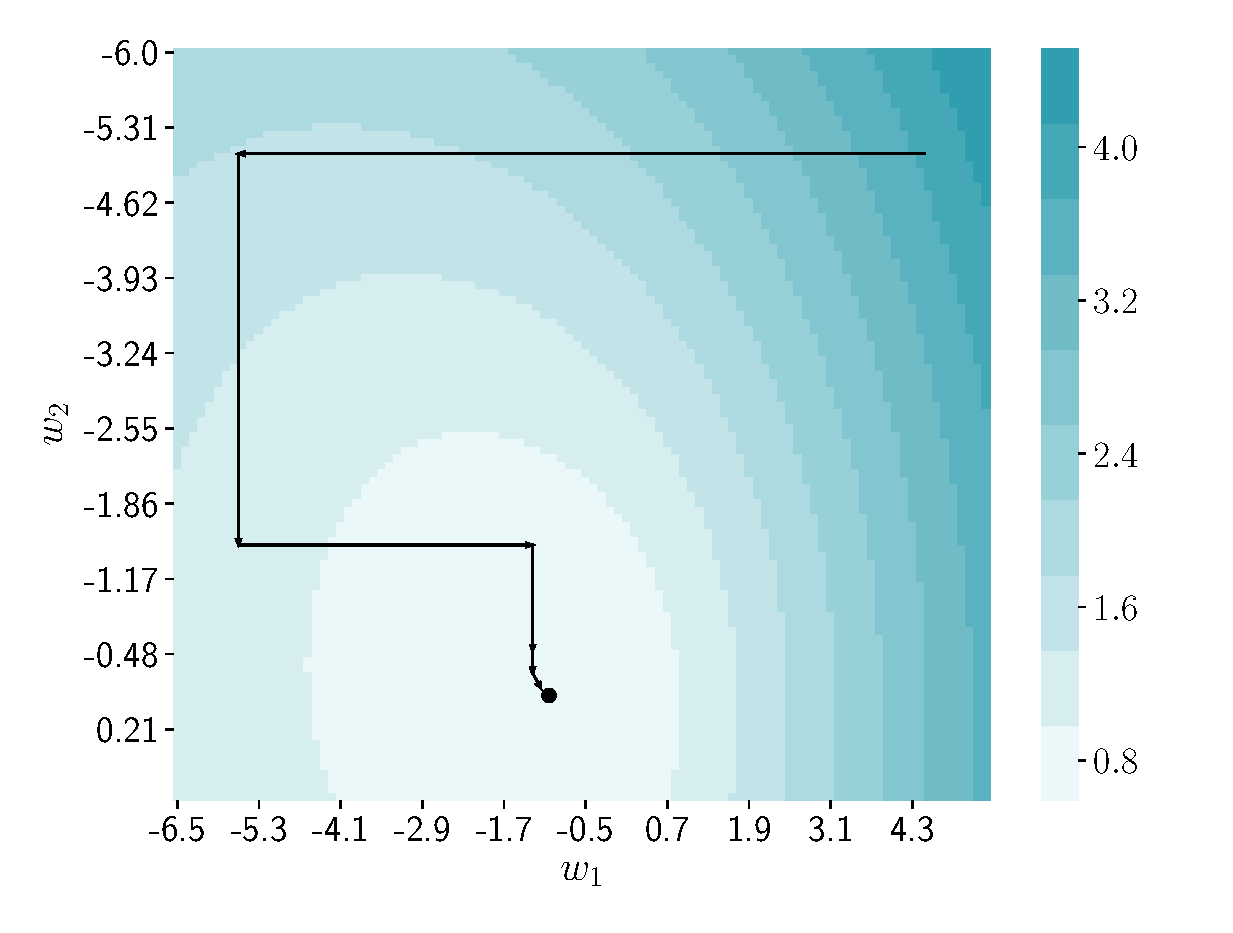
\includegraphics[width=0.6\linewidth]{figs/ch4/irls_qpfs_2d}	 
	\caption{Оптимизационный процесс предложенного метода QPFS+Ньютон для модели логистической регрессии}
	\label{ch4:fig:irls_qpfs_2d}
\end{figure}

На Рис.~\ref{ch4:fig:active_params_wrt_iters} показаны наборы активных параметров на итерациях для набора данных Boston Housing и нейронной сети с двумя скрытыми нейронами. 
Темные ячейки соответствуют активным параметрам, которые мы оптимизируем.
 
\begin{figure}
	\centering
	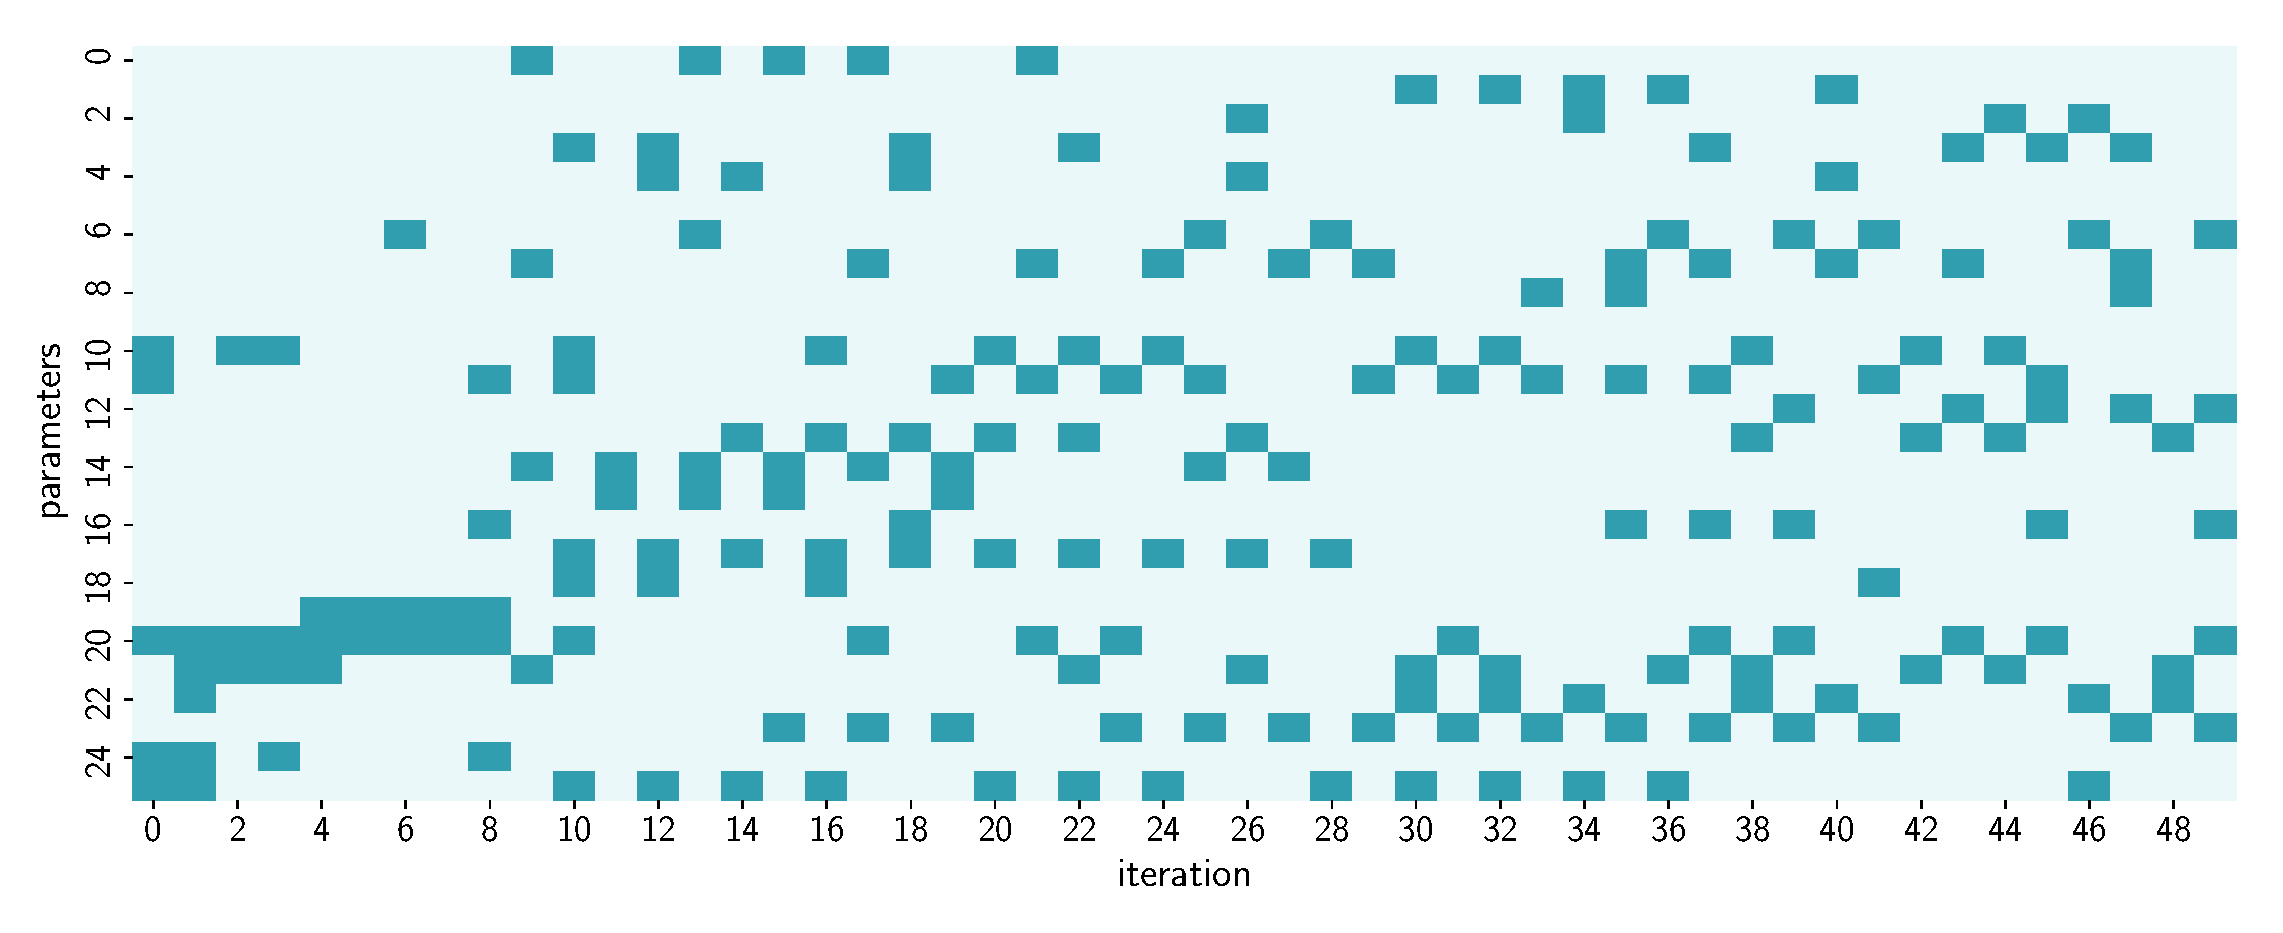
\includegraphics[width=\linewidth]{figs/ch4/active_params_wrt_iters}	
	\caption{Множество активных параметров на протяжении оптимизационного процесса}
	\label{ch4:fig:active_params_wrt_iters}
\end{figure}

В рассмотренных примерах число обусловленности~$\kappa(\bH)$ для метода Ньютона на некоторых итерациях было чрезвычайно большим. 
Выбор активных параметров позволил значительно сократить число обусловленности. 

Приведём сравнение предложенного метода с существующими методами, а именно градиентным спуском~(GD), моментом Нестерова~\cite{nesterov1983momentum}, Adam~\cite{kingma2014adam} и оригинальным методом Ньютона. 
Проведены эксперименты для моделей нелинейной и логистической регрессий. 
Наборы данных были выбраны из репозитория UCI~\cite{uci2017}. 
Результаты показаны в таблицах~\ref{ch4:tbl:nonlin_reg_results} и \ref{ch4:tbl:log_reg_results}. 
Для каждого набора данных две строки таблиц содержат ошибки для тренировочной~(первая строка) и тестовой~(вторая строка) выборок. 
В таблице~\ref{ch4:tbl:nonlin_reg_results} приведена квадратичная ошибка, в таблице~\ref{ch4:tbl:log_reg_results}~--- кросс-энтропия.
Чтобы найти среднюю ошибку и ее стандартное отклонение использовалась процедура кросс валидации с разбиением на 5 фолдов. 
Предложенный метод показывает меньшую ошибку на трех из четырех наборов данных для нелинейной регрессии и на двух из трех наборов данных для логистической регрессии.

\begin{table}[h]
\footnotesize
	\caption{Средняя квадратичная ошибка рассматриваемых алгоритмов оптимизации для модели нелинейной регрессии}
	\label{ch4:tbl:nonlin_reg_results}
	\centering
	\begin{tabular}{|l|c|c|c|c|c|c|}
		\hline
		Выборка & \begin{tabular}[c]{@{}c@{}}\ $m$ \\ \ $n$ \end{tabular} 
		& GD 
		& Нестеров 
		& ADAM 
		& Ньютон 
		&
		\begin{tabular}[c]{@{}c@{}}QPFS+Ньютон\\ \end{tabular} \\ 
		\hline
		Boston House
		& 506
		& $27.2\pm4.6$
		& $46.0\pm11.0$
		& $35.4\pm2.5$           
		& $22.1\pm15.2$            
		& $20.9\pm10.4$   \\  
		Prices
		&\multicolumn{1}{c|}{13}
		& \multicolumn{1}{c|}{$32.4\pm5.6$}
		& \multicolumn{1}{c|}{$53.3\pm11.5$}
		& \multicolumn{1}{c|}{$37.8\pm7.0$}
		& \multicolumn{1}{c|}{$28.9\pm13.6$}
		& \multicolumn{1}{c|}{$\mathbf{24.5\pm9.4}$}\\ 
		\hline
		Communities
		& 1994
		& $48.0\pm6.4$
		& $31.4\pm2.8$
		& $23.3\pm3.7$        
		& $18.3\pm3.4$          
		&  $26.7\pm3.1$  \\ 
		and Crime
		&\multicolumn{1}{c|}{99}
		& \multicolumn{1}{c|}{$47,5\pm6.5$}
		& \multicolumn{1}{c|}{$32.9\pm4.3$}
		& \multicolumn{1}{c|}{$28,1\pm4.5$}
		& \multicolumn{1}{c|}{$28.8\pm3.6$}
		& \multicolumn{1}{c|}{$\mathbf{28.4\pm3.0}$} \\ 
		\hline
		Forest
		& 517
		& $18.9\pm0.4$
		& $1.83\pm0.4$
		& $1.81\pm0.6$             
		& $17.7\pm0.4$             
		& $17.9\pm0.4$   \\ 
		Fires
		&\multicolumn{1}{c|}{10}
		& \multicolumn{1}{c|}{$\mathbf{20.0\pm2.1}$}
		& \multicolumn{1}{c|}{ $20.2\pm2.2$}
		& \multicolumn{1}{c|}{ $\mathbf{20.0\pm2.0}$}
		& \multicolumn{1}{c|}{ $20.6\pm1.4$}
		& \multicolumn{1}{c|}{ $20.2\pm2.2$} \\ 
		\hline
		Residential
		& 372
		&  $51.6\pm17.7$
		&  $32.6\pm19.5$
		&  $30.0\pm24.8$            
		&  $35.5\pm24.7$            
		&   $30.3\pm10.7$ \\ 
		Building
		&\multicolumn{1}{c|}{103}
		& \multicolumn{1}{c|}{ $53.7\pm13.9$}
		& \multicolumn{1}{c|}{ $34.1\pm13.6$}
		& \multicolumn{1}{c|}{ $34.1\pm19.4$}
		& \multicolumn{1}{c|}{ $35.0\pm15.6$}
		& \multicolumn{1}{c|}{ $\mathbf{30.9\pm5.3}$} \\ 
		\hline
	\end{tabular}
\end{table}

\begin{table}[h]
\footnotesize
	\caption{Среднее значение кросс-энтропии рассматриваемых алгоритмов оптимизации для модели логистической регрессии}
	\label{ch4:tbl:log_reg_results}
	\centering
	\begin{tabular}{|l|c|c|c|c|c|c|}
		\hline
		Выборка & \begin{tabular}[c]{@{}c@{}}\ $m$ \\ \ $n$ \end{tabular} 
		& GD 
		& Нестеров 
		& ADAM 
		& Ньютон 
		&
		\begin{tabular}[c]{@{}c@{}}QPFS+Ньютон\\ \end{tabular} \\ 
		\hline
		Breast
		& 569
		& $0.6\pm0.1$
		& $0.4\pm0.1$
		& $0.8\pm0.2$           
		& $0.3\pm0.1$            
		& $0.2\pm0.1$   \\  
		Cancer
		&\multicolumn{1}{c|}{30}
		& \multicolumn{1}{c|}{$\mathbf{0.9\pm0.2}$}
		& \multicolumn{1}{c|}{$1.0\pm0.7$}
		& \multicolumn{1}{c|}{$1.2\pm0.2$}
		& \multicolumn{1}{c|}{$1.0\pm0.2$}
		& \multicolumn{1}{c|}{$1.1\pm0.3$}\\ 
		\hline
		Cardiotocography
		& 2126
		& $11.5\pm4.7$
		& $11.5\pm4.7$
		& $8.8\pm4.4$        
		& $11.5\pm5.7$          
		&  $7.7\pm4.2$  \\
		
		&\multicolumn{1}{c|}{21}
		& \multicolumn{1}{c|}{$11.6\pm5.8$}
		& \multicolumn{1}{c|}{$11.5\pm5.7$}
		& \multicolumn{1}{c|}{$9.0\pm2.6$}
		& \multicolumn{1}{c|}{$11.5\pm4.7$}
		& \multicolumn{1}{c|}{$\mathbf{7.7\pm4.7}$} \\ 
		\hline
		Climate Model
		& 540
		& $1.2\pm0.1$
		& $1.0\pm0.2$
		& $1.5\pm0.2$             
		& $1.0\pm0.5$             
		& $0.8\pm0.3$   \\ 
		Simulation Crashes
		&\multicolumn{1}{c|}{18}
		& \multicolumn{1}{c|}{$1.4\pm2.0$}
		& \multicolumn{1}{c|}{ $1.3\pm0.7$}
		& \multicolumn{1}{c|}{ $1.8\pm0.3$}
		& \multicolumn{1}{c|}{ $1.2\pm0.5$}
		& \multicolumn{1}{c|}{ $\mathbf{1.1\pm0.4}$} \\ 
		\hline
	\end{tabular}
\end{table}



\newpage{}
\chapter{Порождение признаков с помощью метамоделей}


\section{Постановка задачи}
Временные ряды акселерометра образуют множество~$\mathcal{S}$ сегментов~$s$ фиксированной длины~$T$:
\begin{equation}
s = [x_1, \dots, x_T]^{T} \in \bbR^T.
\label{ch5:eq:time_series}
\end{equation}
Необходимо построить модель классификации~$f: \bbR^T \rightarrow Y$, которая будет ставить в соответствие каждому сегменту из множества~$\mathcal{S}$ метку класса из конечного множества~$Y$.
Обозначим за
\begin{equation}
	\mathcal{D} = \{(s_i, y_i)\}_{i=1}^m
	\label{ch5:eq:sample}
\end{equation}
исходная выборка, где $s_i \in \mathcal{S}$ и $y_i = f(s_i)\in Y$.

Авторы предлагают построить модель~$f$ в в де суперпозиции $f=f(\mathbf{g})$.
Функция $\mathbf{g}: \bbR^T \rightarrow \bbR^n$ является отображением из пространства~$\bbR^{T} $ в признаковое пространство~$G \subset \bbR^n$.
Имея функцию порождения признаков~$\mathbf{g}$, преобразуем исходную выборку~\eqref{ch5:eq:sample} в
\[
	\mathcal{D}_G = \{(\mathbf{g}_i, y_i)\}_{i=1}^m,
\]
где $\mathbf{g}_i = \mathbf{g}(s_i) \in G$. 

Модель классификации $f=f(\mathbf{g}, \mathbf{\theta})$ параметризована вектором~$\boldsymbol{\theta}$. 
Оптимальные параметры~$\hat{\mathbf{\theta}}$ определяются оптимизацией функции ошибки классификации
\begin{equation}
\hat{\mathbf{\theta}} = \argmin_{\mathbf{\theta}} L(\mathbf{\theta}, \mathcal{D}_G, \mathbf{\mu}).
\label{ch5:eq:optimal_classification_params}
\end{equation}
Вектор~$\mathbf{\mu}$ является внешним параметром для заданной модели классификации. 
Примеры таких параметров и функций ошибки для различных моделей классификации приведены ниже.

Чтобы сравнить качество классификации с прошлыми результатами~\cite{karasikov2016feature,ivkin2015ts}, в качестве метрики качества используется точность классификации:
\begin{equation}
	\mathrm{accuracy} = \frac{1}{m} \sum_{i=1}^{m} \left[f\left(\mathbf{g}(s_i), \hat{\mathbf{\theta}} \right)= y_i\right].
	\label{ch5:eq:accuracy}
\end{equation}

\section{Порождение признаков}

Цель данной работы~--- провести сравнение различных подходов к генерации признаков.
В этом разделе проводится анализ рассматриваемых методов.

\subsubsection{Экспертные функции.}
В качестве базового подхода будем использовать экспертные функции как функции порождения признаков.
Экспертные функции~--- это некоторые статистики~$g_j$, где $g_j: \bbR^T \rightarrow \bbR$.
Признаковым описанием~$\mathbf{g}(s)$ объекта~$s$ являются значения заданных экспертных статистик для данного объекта
\[
\mathbf{g}(s) = [g_1(s), \dots, g_n(s)]^{\T}.
\]

В работе~\cite{kwapisz2011activity} авторы предлагают использовать экспертные функции, приведенные в таблице~\ref{ch5:tbl:expert_functions}.
Такая процедура порождения признаков генерирует признаковое описание временного ряда~$\mathbf{g}(s) \in \bbR^{40}$.

\begin{table}[ht]
	\centering
	\caption{Expert functions}
	\begin{tabular}{|l|c|}
		\hline
		\textbf{Function description}    & \textbf{Formula} \\ \hline
		Mean                    & $\bar{x} = \frac{1}{T} \sum_{t=1}^{T} x_t$    \\ \hline
		Standard deviation      & $\sqrt{\frac{1}{T} \sum_{t=1}^{T} (x_t - \bar{x})^2}$    \\ \hline
		Mean absolute deviation & $\frac{1}{T} \sum_{t=1}^{T} |x_t - \bar{x}|$    \\ \hline
		Distribution            &  Histogram values with 10 bins    \\ \hline
	\end{tabular}
	\label{ch5:tbl:expert_functions}
\end{table}

\subsubsection{Авторегрессионная модель.}
Авторегрессионная модель~\cite{lukashin2003adaptive} порядка $n$
использует параметрическую модель для аппроксимации временного ряда $s$. 
Каждое значение временного ряда приближается линейной комбинацией предыдущих $n-1$ значений
\begin{equation*}
x_t = w_0 + \sum_{j=1}^{n-1} w_j x_{t-j} + \epsilon_t,
\end{equation*}
где $\epsilon_t$~--- регрессионные остатки.
Оптимальные параметры $\hat{\mathbf{w}}$ авторегрессионной модели используются как признаки $\mathbf{g}(s)$.
Данные параметры минимизируют квадратичную ошибку аппроксимации временного ряда и предсказания модели

\begin{equation}
\mathbf{g}(s) = \hat{\mathbf{w}} = \argmin_{\mathbf{w} \in \bbR^{n}} \left( \sum_{t=n}^{T} \|x_t - \hat{x}_t\|^2\right).
\label{ch5:eq:autoregressive_description}
\end{equation}
Задача~\eqref{ch5:eq:autoregressive_description} эквивалентна задаче линейной регрессии.
Поэтому для каждого временного ряда~$s$ необходимо решить задачу линейной регрессии размера $n$.
Пример аппроксимации временного ряда авторегрессионной моделью представлен на Рис.~\ref{ch5:fig:ar_example}.

\begin{figure}[ht]
	\centering
	\includegraphics[width=1\linewidth]{figs/ch5/ar_example.png}
	\caption{Time series approximation using autoregressive model with order $n = 20$}
	\label{ch5:fig:ar_example}
\end{figure}

\subsubsection{Анализ сингулярного спектра.}
Альтернативной гипотезой порождения признакового пространства для временного ряда является анализ сингулярного спектра (Singular Spectrum Analysis, SSA)~\cite{hassani2007singular}. 
Для каждого временного ряда $s$ из выборки $\mathcal{D}$ строится траекторная матрица:
\[
\mathbf{X} = 
\begin{pmatrix}
x_1 & x_2 & \dots & x_n \\
x_2 & x_3 & \dots & x_{n+1} \\
\dots & \dots & \dots & \dots \\
x_{T-n+1} & x_{T-n+2} & \dots & x_T
\end{pmatrix}.
\]
Здесь ширина окна $n$ является внешним структурным параметром.
Сингулярное разложение матрицы $\mathbf{X}^{\T} \mathbf{X}$:
\[
\mathbf{X}^{\T} \mathbf{X} = \mathbf{U} \mathbf{\Lambda} \mathbf{U}^{\T},
\]
где $\mathbf{U}$~--- унитарная матрица и $\Lambda = \mathrm{diag}(\lambda_1, \dots, \lambda_n)$ причём $\lambda_i$ собственные значения $\mathbf{X}^{\T} \mathbf{X}$. 
Признаковое описание объекта $s$ задаётся спектром матрицы $\mathbf{X}^{\T} \mathbf{X}$:
\[
\mathbf{g}(s) = \left[\lambda_1, \dots, \lambda_n\right]^{\T}.
\]
\subsubsection{Spline Approximation.}
Предлагаемый метод аппроксимирует временные ряды с помощью сплайнов~\cite{deboor1978splines}. Сплайн определяется его параметрами: узлами и коэффициентами.
Предполагается, что узлы сплайна $\{\xi_\ell\}_{\ell=0}^M$ равномерно распределены по временной оси.
Кусочные модели, построенные на отрезках $[\xi_{\ell-1}; \xi_{\ell}]$, заданы коэффициентами $\{\mathbf{w}_\ell\}_{\ell=1}^{M}$.
\begin{figure}[h]
	\centering
	\includegraphics[width=1\linewidth]{figs/ch5/spline_example.png}
	\caption{Time series approximation using three order splines}
	\label{ch5:fig:spline_example}
\end{figure}
Оптимальные параметры сплайна являются решением системы с дополнительными условиями равенства производных до второго порядка включительно на концах отрезков.
Обозначим каждый отрезок-сегмент $p_i(t)$ $i = 1, \dots, M$ и весь сплайн $S(t)$. Тогда система уравнений принимает вид
\begin{align*}
S(t) &= \begin{cases}
p_1(t) = w_{10} +w_{11}t + w_{12}t^2 + w_{13}t^3, & t\in [\xi_0, \xi_1],\\
p_2(t) = w_{20} +w_{21}t + w_{22}t^2 + w_{23}t^3, & t\in [\xi_1, \xi_2],\\
\cdots&\cdots \\
p_{M}(t) = w_{L0} +w_{M1}t + w_{M2}t^2 + w_{M3}t^3, & t\in [\xi_{M-1}, \xi_M],					
\end{cases}
\end{align*}
%For $S(t)$ to be an interpolatory cubic spline, we must also have conditions:
\begin{align*}
S(\xi_t) &= x_t, \quad t = 0, \dots, M,\\
p_i'(\xi_i) &= p_{i+1}'(\xi_i),\: p_i''(\xi_i) = p_{i+1}''(\xi_i), \quad i = 1, \dots, M-1,\\
p_i(\xi_{i-1}) &= x_{i-1},\: p_i(\xi_i) = x_i, \quad i = 1, \dots, M.
\end{align*}
Объединение всех параметров сплайна задаёт признаковое описание временного ряда:
\[
\mathbf{g}(s) = \left[\mathbf{w}_1, \dots, \mathbf{w}_{M}\right]^{\T}.
\]

Рис.~\ref{ch5:fig:spline_example} показывает аппроксимацию временного ряда с использованием модели сплайнов.
По сравнению с авторегрессионной моделью сплайны строят более гладкую аппроксимацию, используя такое же количество параметров.

\section{Классификация временных рядов}
Для классификации временных рядов будем использовать подход один против всех. 
Для каждого класса обучается бинарный классификатор, и на стадии предсказания объект классифицируется согласно наиболее уверенному классификатору.
Использовались три модели классификации: логистическая регрессия, SVM и случайный лес.

\subsubsection{Логистическая регрессия.}
Оптимальные параметры модели $\hat{\mathbf{w}}, \hat{b}$  в случае логистической регрессии определяются минимизацией функции ошибки~\eqref{ch5:eq:optimal_classification_params}

\begin{equation*}
L(\mathbf{\theta}, \mathcal{D}_G, \mu) = \sum_{i=1}^{m} \log\bigl(1 + \exp(-y_i [\mathbf{w}^{\T} \mathbf{g}_i + b])\bigl) + \frac{\mu}{2} \|\mathbf{w}\|^2, \:\:\mbox{where}\:\: \mathbf{\theta}  = \begin{bmatrix}
\mathbf{w} \\ b
\end{bmatrix}.
\end{equation*}

Решающее правило $f(\mathbf{g}, \mathbf{\theta})$~--- знак линейной комбинации описания объекта $\mathbf{g}$ и параметров $\hat{\mathbf{\theta}}$
\begin{equation*}
\hat{y} = f(\mathbf{g}, \hat{\mathbf{\theta}}) = \sgn(\mathbf{g}^{\T} \hat{\mathbf{w}} + \hat{b}).
\end{equation*}

\subsubsection{SVM.}
Оптимизационная задача метода SVM имеет вид
\begin{align*}
\hat{\mathbf{\theta}}  = \begin{pmatrix}
\hat{\mathbf{w}} \\ \hat{b} \\ \hat{\mathbf{\xi}}
\end{pmatrix}= \argmin_{\mathbf{w}, b, \mathbf{\xi}}  \frac{1}{2} \|\mathbf{w}\|^2 + \mu \sum_{i=1}^{m} \xi_i,\:\:
\mbox{s.t.} \:\: &y_i \left(\mathbf{w}^{\T} \mathbf{g}_i + b\right) \geq 1 - \xi_i,\\
&\xi_i \geq 0, \quad 1 \leq i \leq m.
\end{align*}
Целевая функция соответствует функции ошибки классификации $L(\mathbf{\theta}, \mathcal{D}_G, \mu)$.
Предсказание для нового объекта вычисляется аналогично $
\hat{y} = \sgn (\mathbf{g}^{\T} \hat{\mathbf{w}} + \hat{b})$.

\subsubsection{Случайный лес.}
Случайный лес использует идею бэггинга. 
Идея состоит в построении многих слабых, неустойчивых классификатов на подвыборках с возвращениями и усреднения их предсказаний.
Метод предполагает использование в качестве базовых классификаторов моделей с низким смещением и высокой дисперсией. 
Усреднение позволяет уменьшить дисперсию.
В случае случайного леса базовой моделью выступают решающие деревья. Идея бэггинга используется не только для самих объектов, но и для множества признаков.
В данном случае предсказание для нового объекта получается усреднением всех предсказаний отдельных деревьев:

\begin{equation*}
\hat{y} = \sgn \left(\frac{1}{B} \sum_{i=1}^{B} \text{pred}(\mathbf{g}_i) \right),
\end{equation*}
где $B$~--- количество деревьев в композиции.


\section{Эксперимент}
В данной работе эксперименты проводились на двух датасетах временных рядов акселерометра мобильного телефона: WISDM~\cite{wisdm} и USC-HAD~\cite{usc}. 
Акселерометр мобильного телефона проводит измерение ускорения по трём осям с частотой 100 Hz.
Данные WISDM содержат 4321 временной ряд.
Каждый временной ряд прнадлежит к одному из 6 классов. 
Данные USC-HAD содержат 13620 временных рядов, принадлежащих одному из 12 классов.  
В таблице~\ref{ch5:tbl:activities_distributions} представлено распределение временных рядов по классам для каждого датасета.
Длина временного ряда равна 200.
На рис.~\ref{ch5:fig:ts_example} представлен пример одного из временных рядов.

\begin{table}[!ht]
	\centering
	\caption{Distributions of the classes}
	\subfloat[WISDM]{
		\begin{tabular}{r|l|rr}
			\hline
			&\textbf{Activity}   & \multicolumn{2}{l}{\textbf{\# objects}} \\
			\hline
			1&Standing            &229      &5.30  \% \\
			2&Walking             &1917     &44.36 \% \\
			3&Upstairs            &466      &10.78 \% \\
			4&Sitting             &277      &6.41  \% \\
			5&Jogging             &1075     &24.88 \% \\
			6&Downstairs          &357      &8.26  \% \\
			\hline
			&Total & \multicolumn{2}{l}{4321}  \\
			\hline
	\end{tabular}}
	\hspace{0.5cm}
	\subfloat[USC-HAD]{
		\begin{tabular}{r|l|rr}
			\hline
			&\textbf{Activity} & \multicolumn{2}{l}{\textbf{\# objects}} \\ \hline
			1&Standing            &1167     &8.57  \% \\
			2&Elevator-up         &764      &5.61  \% \\
			3&Walking-forward     &1874     &13.76 \% \\
			4&Sitting             &1294     &9.50  \% \\
			5&Walking-downstairs  &951      &6.98  \% \\
			6&Sleeping            &1860     &13.66 \% \\
			7&Elevator-down       &763      &5.60  \% \\
			8&Walking-upstairs    &1018     &7.47  \% \\
			9&Jumping             &495      &3.63  \% \\
			10&Walking-right       &1305     &9.58  \% \\
			11&Walking-left        &1280     &9.40  \% \\
			12&Running             &849      &6.23  \% \\
			\hline 
			&Total              & \multicolumn{2}{l}{13620}\\ 
			\hline
	\end{tabular}}
	\label{ch5:tbl:activities_distributions}
\end{table}

\begin{figure}[!ht]
	\centering
	\includegraphics[width=1\linewidth]{figs/ch5/ts_example.png}
	\caption{Time series example}
	\label{ch5:fig:ts_example}
\end{figure}

\begin{figure}[!ht]
	\centering
	\subfloat{
		\includegraphics[width=0.49\linewidth]{figs/ch5/wisdm_methods.png}}
	\subfloat{
		\includegraphics[width=0.49\linewidth]{figs/ch5/uschad_methods.png}}
	\caption{Multiclass accuracy score}
	\label{ch5:fig:accuracy_results}
\end{figure}

В эксперименте для каждого датасета были порождены признаки одним из методов: экспертные функции, авторегрессионная модель, SSA и сплайны.
Для каждой процедуры порождения признаквого описания настроивались три модели классификации: логистическая регрессия, SVM и случайный лес.
Внешние структурные параметры (длина авторегрессионной модели $n$, ширина окна SSA $n$, число узлов сплайна $M$) настраивались процедурой кросс-валидации:
\begin{align}\label{cv}
CV(K) = \frac{1}{K}\sum_{k=1}^{K} L(f_k, \mathcal{D}\setminus \mathcal{C}_k),
\end{align}
где $C_k$~---$\frac{K-1}{K}$ доля от всей выборки, используемая для обучения модели $f_k$.
Гиперпараметры $\boldsymbol{\mu}$ моделей классификации были настроаны той же процедурой кросс-валидации.

Первый подход к порождению признаков временных рядов~---экспертные функции.
Основной недостаток такого подхода необходимость экспертного задания функций	 и возможности вычисления их для конкретного датасета.

Авторегрессионная модель требует задания параметра длины модели $n$. 
Процедура кросс-валидации дала наибольшее качество при $n=20$ для обоих датасетов.

Модель SSA была настроена аналошгичной процедурой выбора оптимальных гиперпараметров. Конечная модель имела ширину окна $n=20$.

\begin{figure}[!ht]
	\centering
	\subfloat[WISDM dataset]{
		\includegraphics[width=0.33\linewidth]{figs/ch5/hist_wisdm_lr_all.png}}
	\subfloat[USC-HAD dataset]{
		\includegraphics[width=0.66\linewidth]{figs/ch5/hist_uschad_lr_all.png}}\\
	\subfloat[WISDM dataset]{
		\includegraphics[width=0.33\linewidth]{figs/ch5/hist_wisdm_rf_all.png}}
	\subfloat[USC-HAD dataset]{
		\includegraphics[width=0.66\linewidth]{figs/ch5/hist_uschad_rf_all.png}}\\
	\subfloat[WISDM dataset]{
		\includegraphics[width=0.33\linewidth]{figs/ch5/hist_wisdm_svm_all.png}}
	\subfloat[USC-HAD dataset]{
		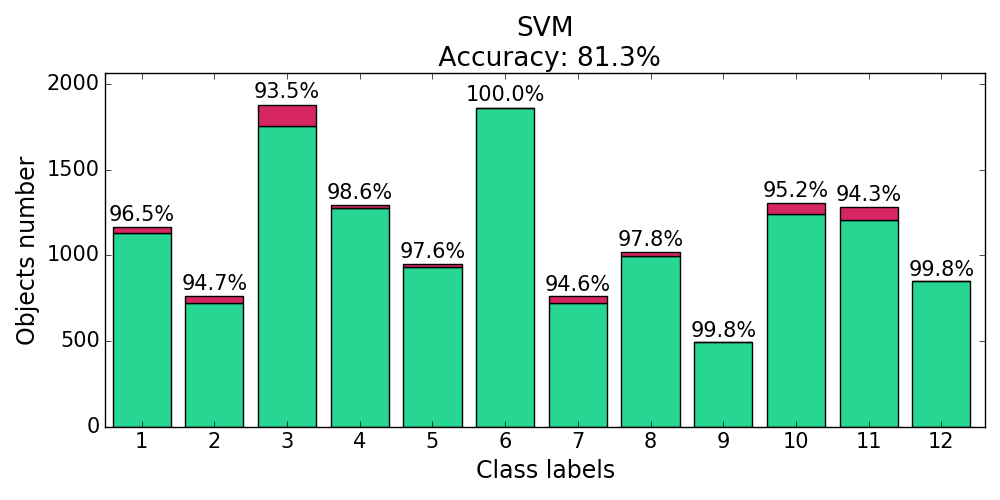
\includegraphics[width=0.66\linewidth]{figs/ch5/hist_uschad_svm_all.png}}\\
	\caption{Accuracy scores of classification of each class using all features}
	\label{ch5:fig:feature_union_results}
\end{figure}

Для аппроксимации временных рядов кубическими сплайнами~\cite{deboor1978splines} использовалась библиотека $scipy$. 
Узлы сплайнов $\{\xi_{\ell}\}_{\ell = 1}^M$ были распределены равномерно по временной оси.
Значение параметра $M$ было подобрано на кросс-валидации.

Для обоих датасетов процедуры порождения признаковых описаний дали следующие количества признаков: экспертные функции~---40; авторегрессионная модель~---60; анализ сингулярного спектра~---60; сплайны~---33.

\begin{table}[!ht]
	\centering
	\caption{Binary accuracy scores for WISDM using different feature generation methods: EX~--- Expert, AR~--- Auto-Reg, SSA and  SPL for Splines}
	\footnotesize
	\begin{tabular}{r|rrrr|rrrr|rrrr|}
		& \multicolumn{4}{c|}{\textbf{Logistic Regression}} & \multicolumn{4}{c|}{\textbf{Random Forest}} & \multicolumn{4}{c|}{\textbf{SVM}}          \\ \cline{2-13} 
		& EX   & AR   & SSA   & SPL  & EX  & AR & SSA & SPL & EX & AR & SSA & SPL \\ \hline
		All& 0.85 & 0.91 & 0.84 & 0.58 & 0.93 & 0.93 & 0.92 & 0.79 & 0.93 & 0.95 & 0.95 & 0.77 \\
		Standing& 0.99 & 0.98 & 1.00 & 0.95 & 1.00 & 0.99 & 1.00 & 0.99 & 0.99 & 0.98 & 1.00 & 0.96 \\
		Walking& 0.91 & 0.96 & 0.86 & 0.61 & 0.96 & 0.97 & 0.95 & 0.86 & 0.96 & 0.98 & 0.98 & 0.84 \\
		Upstairs& 0.91 & 0.95 & 0.91 & 0.89 & 0.96 & 0.96 & 0.96 & 0.90 & 0.96 & 0.98 & 0.97 & 0.89 \\
		Sitting& 0.99 & 0.98 & 1.00 & 0.99 & 1.00 & 0.99 & 1.00 & 1.00 & 0.99 & 0.98 & 1.00 & 1.00 \\
		Jogging& 0.98 & 0.99 & 0.99 & 0.80 & 0.99 & 0.99 & 0.99 & 0.92 & 0.99 & 0.99 & 0.99 & 0.93 \\
		Downstairs& 0.93 & 0.96 & 0.94 & 0.92 & 0.96 & 0.97 & 0.96 & 0.92 & 0.96 & 0.98 & 0.97 & 0.92 \\ \hline
	\end{tabular}
	\label{ch5:tbl:wisdm_methods_results}
\end{table}

\begin{table}[!ht]
	\centering
	\footnotesize
	\caption{Binary accuracy scores for USC-HAD using different feature generation methods: EX~--- Expert, AR~--- Auto-Reg, SSA and  SPL for Splines}
	\label{my-label}
	\begin{tabular}{r|rrrr|rrrr|rrrr|}
		& \multicolumn{4}{c|}{\textbf{Logistic Regression}} & \multicolumn{4}{c|}{\textbf{Random Forest}} & \multicolumn{4}{c|}{\textbf{SVM}}          \\ \cline{2-13} 
		& EX   & AR   & SSA   & SPL  & EX  & AR & SSA & SPL & EX & AR & SSA & SPL \\ \hline
		All& 0.67 & 0.65 & 0.64 & 0.41 & 0.87 & 0.70 & 0.84 & 0.74 & 0.80 & 0.65 & 0.82 & 0.74 \\
		Standing& 0.94 & 0.94 & 0.92 & 0.89 & 0.98 & 0.94 & 0.97 & 0.98 & 0.95 & 0.94 & 0.97 & 0.96 \\
		Elevator-up& 0.94 & 0.94 & 0.93 & 0.92 & 0.95 & 0.95 & 0.95 & 0.95 & 0.93 & 0.94 & 0.94 & 0.93 \\
		Walking-forward& 0.87 & 0.87 & 0.89 & 0.70 & 0.97 & 0.89 & 0.96 & 0.88 & 0.95 & 0.87 & 0.97 & 0.91 \\
		Sitting& 0.98 & 0.95 & 0.94 & 0.96 & 0.99 & 0.96 & 0.98 & 0.99 & 0.98 & 0.96 & 0.99 & 0.99 \\
		Walking-downstairs& 0.95 & 0.93 & 0.93 & 0.90 & 0.99 & 0.96 & 0.98 & 0.95 & 0.98 & 0.93 & 0.98 & 0.96 \\
		Sleeping& 1.00 & 0.98 & 0.99 & 1.00 & 1.00 & 0.98 & 1.00 & 1.00 & 1.00 & 0.98 & 1.00 & 1.00 \\
		Elevator-down& 0.94 & 0.94 & 0.94 & 0.91 & 0.95 & 0.95 & 0.95 & 0.95 & 0.93 & 0.94 & 0.94 & 0.93 \\
		Walking-upstairs& 0.94 & 0.95 & 0.93 & 0.92 & 0.98 & 0.95 & 0.98 & 0.96 & 0.98 & 0.95 & 0.98 & 0.96 \\
		Jumping& 0.99 & 0.99 & 1.00 & 0.97 & 1.00 & 0.99 & 1.00 & 0.99 & 1.00 & 0.99 & 0.97 & 0.99 \\
		Walking-right& 0.91 & 0.90 & 0.91 & 0.86 & 0.97 & 0.92 & 0.96 & 0.92 & 0.96 & 0.90 & 0.97 & 0.93 \\
		Walking-left& 0.89 & 0.91 & 0.90 & 0.88 & 0.97 & 0.93 & 0.97 & 0.93 & 0.95 & 0.91 & 0.97 & 0.93 \\
		Running& 0.99 & 0.99 & 0.99 & 0.92 & 1.00 & 0.99 & 1.00 & 0.97 & 1.00 & 1.00 & 0.95 & 0.98\\ \hline
	\end{tabular}
	\label{ch5:tbl:uschad_methods_results}
\end{table}

На рис.~\ref{ch5:fig:accuracy_results} показано качество классификации~\eqref{ch5:eq:accuracy} для двух датасетов.
Для данных WISDM сплайны дали самое слабое качество классификации.
Результаты для экспертных функций, авторегрессионной модели и SSA схожи.
Для данных USC-HAD результат более восприимчив к выбору модели классификации. 
Для обоих датасетов логистическая регрессия продемонстрировала наименьшее качество, SVM и случайный лес показали почти одинаковое качество.
Для датасета USC-HAD модель с использованием аппроксимации сплайнами
показала сравнимое с другими методами качество. 

В Табл.~\ref{ch5:tbl:wisdm_methods_results} и Табл.~\ref{ch5:tbl:uschad_methods_results} представлены результаты классификации~\eqref{ch5:eq:accuracy} для каждого класса в отдельности.
Первая строка в обеих таблицах демонстрирует точность по всем классам для каждой модели и процедуры генерации признаков.
Следующие строки соответствуют бинарным точностям по каждому из классов.
Для данных WISDM лучшее качество имеют наименее активные классы, такие как Standing и Sitting. 
Для USC-HAD заметного выделения качества для определенных классов не наблюдается.

Также был проведён эксперимент с использованием объединённого множества всех 193 сгенерированных признаков.
Результаты представлены на Рис.~\ref{ch5:fig:feature_union_results}. Соответствие между номера классов и видами активности приведено в Табл.~\ref{ch5:tbl:activities_distributions}. 
Объединение признаков для обучения одной модели позволило увеличить качество. 
Для данных WISDM все точности классификации по классам больше $97 \%$, а для USC-HAD выше $93 \%$.


\newpage{}
\chapter{Порождение признаков с помощью метамоделей}
\label{ch:metamodels}

Исходное пространство сигналов в задачах декодирования, а также в задачах анализа временных рядов является крайне избыточным и неинформативным.
Для извлечения информативных признаков в данной главе ставится задача порождения признакового пространства.

%%%%%%%%%%%%%%%%%%%%%%%%%%%%%%%%%%%%%%%%%%%%%%%%
\section{Постановка задачи порождения признакового пространства}
\label{sec:ch6:feature_generation}
%%%%%%%%%%%%%%%%%%%%%%%%%%%%%%%%%%%%%%%%%%%%%%%%

Временные ряды акселерометра образуют множество~$\mathcal{S}$ сегментов~$\bs = [x_1, \dots, x_T]^{\T}$ фиксированной длины~$T$.
Необходимо построить модель классификации~$a: \bbR^T \rightarrow \bbY$, которая будет ставить в соответствие каждому сегменту из множества~$\mathcal{S}$ метку класса из конечного множества~$\bbY = \{1, \dots, K\}$.
Пусть $\{(\bs_i, y_i)\}_{i=1}^m$~--- исходная выборка, где $\bs_i \in \mathcal{S}$ и $y_i = a(\bs_i)\in \bbY$.

В работе предлагается построить модель~$a$ в виде суперпозиции $a = f \circ \mathbf{g}$.
\begin{definition}
	\textit{Порождающей функцией} будем называть функцию $\mathbf{g}: \bbR^T \rightarrow \mathbb{X}$, отображающую исходные временные ряды $\bs$ из пространства~$\bbR^{T} $ в признаковое пространство~$\bbX \subset \bbR^n$.
\end{definition}
Имея порождающую функцию~$\mathbf{g}$, преобразуем исходную выборку в $\{(\bx_i, y_i)\}_{i=1}^m$, где $\bx_i = \mathbf{g}(\bs_i) \in \bbX$. Здесь $\bx_i$ является исходным объектом.

Модель классификации $f=f(\bx, \btheta)$ является параметрической функцией с вектором параметров~$\btheta$. 
Оптимальные параметры~$\btheta^*$ определяются оптимизацией функции ошибки классификации
\begin{equation}
	\btheta^* = \argmin_{\btheta} L(\btheta, \bX, \by, \bmu).
	\label{ch6:eq:optimal_classification_params}
\end{equation}
Вектор~$\bmu$ является внешним параметром для заданной модели классификации. 
Примеры таких параметров и функций ошибки для различных моделей классификации приведены ниже.

Чтобы сравнить качество классификации с прошлыми результатами~\cite{karasikov2016feature,ivkin2015ts}, в качестве метрики качества используется точность классификации:
\begin{equation}
	\mathrm{accuracy} = \frac{1}{m} \sum_{i=1}^{m} \left[f\left(\mathbf{g}(\bs_i), \btheta^* \right)= y_i\right].
	\label{ch6:eq:accuracy}
\end{equation}

%%%%%%%%%%%%%%%%%%%%%%%%%%%%%%%%%%%%%%%%%%%%%%%%
\section{Модели порождения признакового пространства для временных рядов}
\label{sec:ch6:feature_generation_models}
%%%%%%%%%%%%%%%%%%%%%%%%%%%%%%%%%%%%%%%%%%%%%%%%

Цель данной работы~--- провести сравнение различных подходов к генерации признаков.
В этом разделе проводится анализ рассматриваемых методов.

\subsubsection{Экспертные функции.}
В качестве базового подхода будем использовать экспертные функции как функции порождения признаков.
Экспертные функции~--- это некоторые статистики~$g_j$, где $g_j: \bbR^T \rightarrow \bbR$.
Признаковым описанием~$\mathbf{g}(\bs)$ объекта~$\bs$ являются значения заданных экспертных статистик для данного объекта
\[
	\bx = \mathbf{g}(\bs) = [g_1(\bs), \dots, g_n(\bs)]^{\T}.
\]

В работе~\cite{kwapisz2011activity} авторы предлагают использовать экспертные функции, приведенные в таблице~\ref{ch6:tbl:expert_functions}.
Такая процедура порождения признаков генерирует признаковое описание временного ряда~$\bx = \mathbf{g}(\bs) \in \bbR^{40}$.

\begin{table}[ht]
	\centering
	\caption{Примеры экспертных порождающих функций}
	\begin{tabular}{|l|c|}
		\hline
		\textbf{Описание}    & \textbf{Формула} \\ \hline
		Mean                    & $\bar{s} = \frac{1}{T} \sum_{t=1}^{T} s_t$    \\ \hline
		Standard deviation      & $\sqrt{\frac{1}{T} \sum_{t=1}^{T} (s_t - \bar{s})^2}$    \\ \hline
		Mean absolute deviation & $\frac{1}{T} \sum_{t=1}^{T} |s_t - \bar{s}|$    \\ \hline
		Distribution            &  Histogram values with 10 bins    \\ \hline
	\end{tabular}
	\label{ch6:tbl:expert_functions}
\end{table}

\subsubsection{Авторегрессионная модель.}
Авторегрессионная модель~\cite{lukashin2003adaptive} порядка~$n$
использует параметрическую модель для аппроксимации временного ряда~$\bs$:
\begin{equation*}
	x_t = w_0 + \sum_{j=1}^{n-1} w_j x_{t-j} + \epsilon_t,
\end{equation*}
где $\epsilon_t$~--- регрессионные остатки.
Оптимальные параметры $\mathbf{w}^*$ авторегрессионной модели используются как признаки $\mathbf{g}(\bs)$.
Данные параметры минимизируют квадратичную ошибку аппроксимации временного ряда и предсказания модели

\begin{equation}
	\bx = \mathbf{g}(\bs) = \mathbf{w}^* = \argmin_{\mathbf{w} \in \bbR^{n}} \left( \sum_{t=n}^{T} \|x_t - \hat{x}_t\|^2\right).
	\label{ch6:eq:autoregressive_description}
\end{equation}
Задача~\eqref{ch6:eq:autoregressive_description} эквивалентна задаче линейной регрессии.
Поэтому для каждого временного ряда~$s$ необходимо решить задачу линейной регрессии размера $n$.
Пример аппроксимации временного ряда авторегрессионной моделью представлен на Рис.~\ref{ch6:fig:ar_example}.

\begin{figure}[ht]
	\centering
	\includegraphics[width=1\linewidth]{figs/ch6/ar_example.png}
	\caption{Пример аппроксимации временного ряда авторегрессионной моделью с $n = 20$}
	\label{ch6:fig:ar_example}
\end{figure}

\subsubsection{Анализ сингулярного спектра.}
Для каждого временного ряда~$\bs$ из исходной выборки строится траекторная матрица:
\[
	\bS = 
	\begin{pmatrix}
		s_1 & s_2 & \dots & s_n \\
		s_2 & s_3 & \dots & s_{n+1} \\
		\dots & \dots & \dots & \dots \\
		s_{T-n+1} & s_{T-n+2} & \dots & s_T
	\end{pmatrix}.
\]
Здесь ширина окна $n$ является внешним структурным параметром.
Сингулярное разложение матрицы $\mathbf{S}^{\T} \mathbf{S}$:
\[
\bS^{\T} \bS = \bU \boldsymbol{\Lambda} \bU^{\T},
\]
где $\mathbf{U}$~--- унитарная матрица и $\boldsymbol{\Lambda} = \mathrm{diag}(\lambda_1, \dots, \lambda_n)$ причём $\lambda_i$ собственные значения $\bS^{\T} \bS$. 
Признаковое описание объекта~$\bs$ задаётся спектром матрицы~$\bS^{\T} \bS$:
\[
	\bx = \mathbf{g}(\bs) = \left[\lambda_1, \dots, \lambda_n\right]^{\T}.
\]

\subsubsection{Аппроксимация сплайнами.}
Предлагаемый метод аппроксимирует временные ряды с помощью сплайнов~\cite{deboor1978splines}. Сплайн определяется его параметрами: узлами и коэффициентами.
Предполагается, что узлы сплайна $\{\xi_\ell\}_{\ell=0}^M$ равномерно распределены по временной оси.
Кусочные модели, построенные на отрезках $[\xi_{\ell-1}; \xi_{\ell}]$, заданы коэффициентами $\{\mathbf{w}_\ell\}_{\ell=1}^{M}$.
\begin{figure}[h]
	\centering
	\includegraphics[width=1\linewidth]{figs/ch6/spline_example.png}
	\caption{Пример аппроксимации временного ряда с помощью сплайнов третьего порядка}
	\label{ch6:fig:spline_example}
\end{figure}
Оптимальные параметры сплайна являются решением системы с дополнительными условиями равенства производных до второго порядка включительно на концах отрезков.
Обозначим каждый отрезок-сегмент $p_i(t)$ $i = 1, \dots, M$ и весь сплайн $S(t)$. Тогда система уравнений принимает вид
\begin{equation*}
	S(t) = \begin{cases}
		p_1(t) = w_{10} +w_{11}t + w_{12}t^2 + w_{13}t^3, & t\in [\xi_0, \xi_1],\\
		p_2(t) = w_{20} +w_{21}t + w_{22}t^2 + w_{23}t^3, & t\in [\xi_1, \xi_2],\\
		\cdots&\cdots \\
		p_{M}(t) = w_{L0} +w_{M1}t + w_{M2}t^2 + w_{M3}t^3, & t\in [\xi_{M-1}, \xi_M],					
	\end{cases}
\end{equation*}
\begin{align*}
	S(\xi_t) &= x_t, \quad t = 0, \dots, M,\\
	p_i'(\xi_i) &= p_{i+1}'(\xi_i),\: p_i''(\xi_i) = p_{i+1}''(\xi_i), \quad i = 1, \dots, M-1,\\
	p_i(\xi_{i-1}) &= x_{i-1},\: p_i(\xi_i) = x_i, \quad i = 1, \dots, M.
\end{align*}
Объединение всех параметров сплайна задаёт признаковое описание временного ряда:
\[
	\bx = \mathbf{g}(\bs) = \left[\mathbf{w}_1, \dots, \mathbf{w}_{M}\right]^{\T}.
\]

Рис.~\ref{ch6:fig:spline_example} показывает аппроксимацию временного ряда с использованием модели сплайнов.
По сравнению с авторегрессионной моделью сплайны строят более гладкую аппроксимацию, используя такое же количество параметров.

%%%%%%%%%%%%%%%%%%%%%%%%%%%%%%%%%%%%%%%%%%%%%%%%
\section{Классификация временных рядов в порожденном признаковом пространства}
\label{sec:ch6:feature_generation_classification}
%%%%%%%%%%%%%%%%%%%%%%%%%%%%%%%%%%%%%%%%%%%%%%%%

Для классификации временных рядов будем использовать подход один против всех. 
Для каждого класса обучается бинарный классификатор, и на стадии предсказания объект классифицируется согласно наиболее уверенному классификатору.
Использовались три модели классификации: логистическая регрессия, SVM и случайный лес.

\subsubsection{Логистическая регрессия.}
Оптимальные параметры модели $\mathbf{w}^*, b^*$  в случае логистической регрессии определяются минимизацией функции ошибки~\eqref{ch6:eq:optimal_classification_params}

\begin{equation*}
	L(\btheta, \bX, \by, \mu) = \sum_{i=1}^{m} \log\bigl(1 + \exp(-y_i [\mathbf{w}^{\T} \bx_i + b])\bigl) + \frac{\mu}{2} \|\mathbf{w}\|^2, \:\:\mbox{where}\:\: \btheta  = \begin{bmatrix}
	\mathbf{w} \\ b
	\end{bmatrix}.
\end{equation*}

Решающее правило $f(\bx, \btheta)$~--- знак линейной комбинации описания объекта~$\bx$ и параметров $\btheta^*$
\begin{equation*}
	\hat{y} = f(\bx, \btheta^*) = \sgn(\bx^{\T} \mathbf{w}^* + b^*).
\end{equation*}

\subsubsection{SVM.}
Оптимизационная задача метода SVM имеет вид
\begin{align*}
	\btheta^*  = 
	\begin{pmatrix}
		\mathbf{w}^* \\ 
		b^* \\ 
		\hat{\mathbf{\xi}}
	\end{pmatrix}
	= \argmin_{\mathbf{w}, b, \mathbf{\xi}}  \frac{1}{2} \|\mathbf{w}\|^2 + \mu \sum_{i=1}^{m} \xi_i,\:\:
	\mbox{s.t.} \:\: &y_i \left(\mathbf{w}^{\T} \bx_i + b\right) \geq 1 - \xi_i,\\
	&\xi_i \geq 0, \quad 1 \leq i \leq m.
\end{align*}
Целевая функция соответствует функции ошибки классификации $L(\btheta, \bX, \by, \mu)$.
Предсказание для нового объекта вычисляется аналогично $
\hat{y} = \sgn (\bx^{\T} \mathbf{w}^* + b^*)$.

\subsubsection{Случайный лес.}
Случайный лес использует идею бэггинга. 
Идея состоит в построении многих слабых, неустойчивых классификаторов на подвыборках с возвращениями и усреднения их предсказаний.
Метод предполагает использование в качестве базовых классификаторов моделей с низким смещением и высокой дисперсией. 
Усреднение позволяет уменьшить дисперсию.
В случае случайного леса базовой моделью выступают решающие деревья. Идея бэггинга используется не только для самих объектов, но и для множества признаков.
В данном случае предсказание для нового объекта получается усреднением всех предсказаний отдельных деревьев:

\begin{equation*}
	\hat{y} = \sgn \left(\frac{1}{B} \sum_{i=1}^{B} \text{pred}(\bx_i) \right),
\end{equation*}
где $B$~--- количество деревьев в композиции.


%%%%%%%%%%%%%%%%%%%%%%%%%%%%%%%%%%%%%%%%%%%%%%%%
\section{Анализ порожденных признаковых пространств}
\label{sec:ch6:exp_feature_generation}
%%%%%%%%%%%%%%%%%%%%%%%%%%%%%%%%%%%%%%%%%%%%%%%%

В данной работе эксперименты проводились на двух наборах данных временных рядов акселерометра мобильного телефона: WISDM~\cite{wisdm} и USC-HAD~\cite{usc}. 
Акселерометр мобильного телефона проводит измерение ускорения по трём осям с частотой 100 Hz.
Данные WISDM содержат 4321 временной ряд.
Каждый временной ряд принадлежит к одному из 6 классов. 
Данные USC-HAD содержат 13620 временных рядов, принадлежащих одному из 12 классов.  
В таблице~\ref{ch6:tbl:activities_distributions} представлено распределение временных рядов по классам для каждого датасета.
Длина временного ряда равна 200.
На Рис.~\ref{ch6:fig:ts_example} представлен пример одного из временных рядов.

\begin{table}[!ht]
	\centering
	\caption{Распределение объектов по классам для временных рядов акселерометра}
	\subfloat[WISDM]{
		\begin{tabular}{r|l|rr}
			\hline
			&\textbf{Activity}   & \multicolumn{2}{l}{\textbf{\# objects}} \\
			\hline
			1&Standing            &229      &5.30  \% \\
			2&Walking             &1917     &44.36 \% \\
			3&Upstairs            &466      &10.78 \% \\
			4&Sitting             &277      &6.41  \% \\
			5&Jogging             &1075     &24.88 \% \\
			6&Downstairs          &357      &8.26  \% \\
			\hline
			&Total & \multicolumn{2}{l}{4321}  \\
			\hline
	\end{tabular}}
	\hspace{0.5cm}
	\subfloat[USC-HAD]{
		\begin{tabular}{r|l|rr}
			\hline
			&\textbf{Activity} & \multicolumn{2}{l}{\textbf{\# objects}} \\ \hline
			1&Standing            &1167     &8.57  \% \\
			2&Elevator-up         &764      &5.61  \% \\
			3&Walking-forward     &1874     &13.76 \% \\
			4&Sitting             &1294     &9.50  \% \\
			5&Walking-downstairs  &951      &6.98  \% \\
			6&Sleeping            &1860     &13.66 \% \\
			7&Elevator-down       &763      &5.60  \% \\
			8&Walking-upstairs    &1018     &7.47  \% \\
			9&Jumping             &495      &3.63  \% \\
			10&Walking-right       &1305     &9.58  \% \\
			11&Walking-left        &1280     &9.40  \% \\
			12&Running             &849      &6.23  \% \\
			\hline 
			&Total              & \multicolumn{2}{l}{13620}\\ 
			\hline
	\end{tabular}}
	\label{ch6:tbl:activities_distributions}
\end{table}

\begin{figure}[!ht]
	\centering
	\includegraphics[width=1\linewidth]{figs/ch6/ts_example.png}
	\caption{Примеры временных рядов акселерометра для каждой оси}
	\label{ch6:fig:ts_example}
\end{figure}

\begin{figure}[!ht]
	\centering
	\subfloat{
		\includegraphics[width=0.49\linewidth]{figs/ch6/wisdm_methods.png}}
	\subfloat{
		\includegraphics[width=0.49\linewidth]{figs/ch6/uschad_methods.png}}
	\caption{Мультиклассовая точность классификации для различных порожденных признаковых пространств}
	\label{ch6:fig:accuracy_results}
\end{figure}

В эксперименте для каждого набора данных были порождены признаки одним из методов: экспертные функции, авторегрессионная модель, SSA и сплайны.
Для каждой процедуры порождения признакового описания настраивались три модели классификации: логистическая регрессия, SVM и случайный лес.
Внешние структурные параметры (длина авторегрессионной модели $n$, ширина окна SSA $n$, число узлов сплайна $M$) настраивались процедурой кросс-валидации:
\begin{equation*}
	CV(K) = \frac{1}{K}\sum_{k=1}^{K} \cL(f_k, \bX_k, \by_k, \bmu),
\end{equation*}
где $(\bX_k, \by_k)$~---$\frac{K-1}{K}$ доля от всей выборки, используемая для обучения модели $f_k$.
Гиперпараметры $\boldsymbol{\mu}$ моделей классификации были настроены той же процедурой кросс-валидации.

Первый подход к порождению признаков временных рядов~--- экспертные функции.
Основной недостаток такого подхода необходимость экспертного задания функций и возможности их вычисления для конкретного набора данных.

Авторегрессионная модель требует задания параметра длины модели $n$. 
Процедура кросс-валидации дала наибольшее качество при $n=20$ для обоих наборов данных.

Модель SSA была настроена аналогичной процедурой выбора оптимальных гиперпараметров. Конечная модель имела ширину окна $n=20$.

\begin{figure}[!ht]
	\centering
	\subfloat[WISDM dataset]{
		\includegraphics[width=0.33\linewidth]{figs/ch6/hist_wisdm_lr_all.png}}
	\subfloat[USC-HAD dataset]{
		\includegraphics[width=0.66\linewidth]{figs/ch6/hist_uschad_lr_all.png}}\\
	\subfloat[WISDM dataset]{
		\includegraphics[width=0.33\linewidth]{figs/ch6/hist_wisdm_rf_all.png}}
	\subfloat[USC-HAD dataset]{
		\includegraphics[width=0.66\linewidth]{figs/ch6/hist_uschad_rf_all.png}}\\
	\subfloat[WISDM dataset]{
		\includegraphics[width=0.33\linewidth]{figs/ch6/hist_wisdm_svm_all.png}}
	\subfloat[USC-HAD dataset]{
		\includegraphics[width=0.66\linewidth]{figs/ch6/hist_uschad_svm_all.png}}\\
	\caption{Поклассовая точность классификации временных рядов акселерометра}
	\label{ch6:fig:feature_union_results}
\end{figure}

Для аппроксимации временных рядов кубическими сплайнами~\cite{deboor1978splines} использовалась библиотека $scipy$. 
Узлы сплайнов $\{\xi_{\ell}\}_{\ell = 1}^M$ были распределены равномерно по временной оси.
Значение параметра $M$ было подобрано на кросс-валидации.

Для обоих наборов данных процедуры порождения признаковых описаний дали следующие количества признаков: экспертные функции~--- 40; авторегрессионная модель~--- 60; анализ сингулярного спектра~--- 60; сплайны~--- 33.

\begin{table}[!ht]
	\centering
	\caption{Бинарная точность классификации для данных WISDM с использованием рассматриваемых алгоритмов: EX~--- Expert, AR~--- Auto-Reg, SSA and  SPL for Splines}
	\footnotesize
	\begin{tabular}{r|rrrr|rrrr|rrrr|}
		& \multicolumn{4}{c|}{\textbf{Logistic Regression}} & \multicolumn{4}{c|}{\textbf{Random Forest}} & \multicolumn{4}{c|}{\textbf{SVM}}          \\ \cline{2-13} 
		& EX   & AR   & SSA   & SPL  & EX  & AR & SSA & SPL & EX & AR & SSA & SPL \\ \hline
		All& 0.85 & 0.91 & 0.84 & 0.58 & 0.93 & 0.93 & 0.92 & 0.79 & 0.93 & 0.95 & 0.95 & 0.77 \\
		Standing& 0.99 & 0.98 & 1.00 & 0.95 & 1.00 & 0.99 & 1.00 & 0.99 & 0.99 & 0.98 & 1.00 & 0.96 \\
		Walking& 0.91 & 0.96 & 0.86 & 0.61 & 0.96 & 0.97 & 0.95 & 0.86 & 0.96 & 0.98 & 0.98 & 0.84 \\
		Upstairs& 0.91 & 0.95 & 0.91 & 0.89 & 0.96 & 0.96 & 0.96 & 0.90 & 0.96 & 0.98 & 0.97 & 0.89 \\
		Sitting& 0.99 & 0.98 & 1.00 & 0.99 & 1.00 & 0.99 & 1.00 & 1.00 & 0.99 & 0.98 & 1.00 & 1.00 \\
		Jogging& 0.98 & 0.99 & 0.99 & 0.80 & 0.99 & 0.99 & 0.99 & 0.92 & 0.99 & 0.99 & 0.99 & 0.93 \\
		Downstairs& 0.93 & 0.96 & 0.94 & 0.92 & 0.96 & 0.97 & 0.96 & 0.92 & 0.96 & 0.98 & 0.97 & 0.92 \\ \hline
	\end{tabular}
	\label{ch6:tbl:wisdm_methods_results}
\end{table}

\begin{table}[!ht]
	\centering
	\footnotesize
	\caption{Бинарная точность классификации для данных USC-HAD с использованием рассматриваемых алгоритмов: EX~--- Expert, AR~--- Auto-Reg, SSA and  SPL for Splines}
	\label{my-label}
	\begin{tabular}{r|rrrr|rrrr|rrrr|}
		& \multicolumn{4}{c|}{\textbf{Logistic Regression}} & \multicolumn{4}{c|}{\textbf{Random Forest}} & \multicolumn{4}{c|}{\textbf{SVM}}          \\ \cline{2-13} 
		& EX   & AR   & SSA   & SPL  & EX  & AR & SSA & SPL & EX & AR & SSA & SPL \\ \hline
		All& 0.67 & 0.65 & 0.64 & 0.41 & 0.87 & 0.70 & 0.84 & 0.74 & 0.80 & 0.65 & 0.82 & 0.74 \\
		Standing& 0.94 & 0.94 & 0.92 & 0.89 & 0.98 & 0.94 & 0.97 & 0.98 & 0.95 & 0.94 & 0.97 & 0.96 \\
		Elevator-up& 0.94 & 0.94 & 0.93 & 0.92 & 0.95 & 0.95 & 0.95 & 0.95 & 0.93 & 0.94 & 0.94 & 0.93 \\
		Walking-forward& 0.87 & 0.87 & 0.89 & 0.70 & 0.97 & 0.89 & 0.96 & 0.88 & 0.95 & 0.87 & 0.97 & 0.91 \\
		Sitting& 0.98 & 0.95 & 0.94 & 0.96 & 0.99 & 0.96 & 0.98 & 0.99 & 0.98 & 0.96 & 0.99 & 0.99 \\
		Walking-downstairs& 0.95 & 0.93 & 0.93 & 0.90 & 0.99 & 0.96 & 0.98 & 0.95 & 0.98 & 0.93 & 0.98 & 0.96 \\
		Sleeping& 1.00 & 0.98 & 0.99 & 1.00 & 1.00 & 0.98 & 1.00 & 1.00 & 1.00 & 0.98 & 1.00 & 1.00 \\
		Elevator-down& 0.94 & 0.94 & 0.94 & 0.91 & 0.95 & 0.95 & 0.95 & 0.95 & 0.93 & 0.94 & 0.94 & 0.93 \\
		Walking-upstairs& 0.94 & 0.95 & 0.93 & 0.92 & 0.98 & 0.95 & 0.98 & 0.96 & 0.98 & 0.95 & 0.98 & 0.96 \\
		Jumping& 0.99 & 0.99 & 1.00 & 0.97 & 1.00 & 0.99 & 1.00 & 0.99 & 1.00 & 0.99 & 0.97 & 0.99 \\
		Walking-right& 0.91 & 0.90 & 0.91 & 0.86 & 0.97 & 0.92 & 0.96 & 0.92 & 0.96 & 0.90 & 0.97 & 0.93 \\
		Walking-left& 0.89 & 0.91 & 0.90 & 0.88 & 0.97 & 0.93 & 0.97 & 0.93 & 0.95 & 0.91 & 0.97 & 0.93 \\
		Running& 0.99 & 0.99 & 0.99 & 0.92 & 1.00 & 0.99 & 1.00 & 0.97 & 1.00 & 1.00 & 0.95 & 0.98\\ \hline
	\end{tabular}
	\label{ch6:tbl:uschad_methods_results}
\end{table}

На Рис.~\ref{ch6:fig:accuracy_results} показано качество классификации~\eqref{ch6:eq:accuracy} для двух наборов данных.
Для данных WISDM сплайны дали самое слабое качество классификации.
Результаты для экспертных функций, авторегрессионной модели и SSA схожи.
Для данных USC-HAD результат более восприимчив к выбору модели классификации. 
Для обоих наборов данных логистическая регрессия продемонстрировала наименьшее качество, SVM и случайный лес показали почти одинаковое качество.
Для набора данных USC-HAD модель с использованием аппроксимации сплайнами
показала сравнимое с другими методами качество. 

В таблицах~\ref{ch6:tbl:wisdm_methods_results} и~\ref{ch6:tbl:uschad_methods_results} представлены результаты классификации~\eqref{ch6:eq:accuracy} для каждого класса в отдельности.
Первая строка в обеих таблицах демонстрирует точность по всем классам для каждой модели и процедуры генерации признаков.
Следующие строки соответствуют бинарным точностям по каждому из классов.
Для данных WISDM лучшее качество имеют наименее активные классы, такие как Standing и Sitting. 
Для USC-HAD заметного выделения качества для определенных классов не наблюдается.

Также был проведён эксперимент с использованием объединённого множества всех 193 сгенерированных признаков.
Результаты представлены на Рис.~\ref{ch6:fig:feature_union_results}. Соответствие между номера классов и видами активности приведено в таблице~\ref{ch6:tbl:activities_distributions}. 
Объединение признаков для обучения одной модели позволило увеличить качество. 
Для данных WISDM все точности классификации по классам больше $97 \%$, а для USC-HAD выше $93 \%$.


\newpage{}
\addcontentsline{toc}{section}{Заключение}
\chapter*{Заключение}

Основные результаты диссертационной работы заключаются в следующем.

В главе~\ref{ch:intro} введено понятие прогностической модели в пространствах высокой размерности.
Поставлена формальная задача декодирования сигналов.
Приведён обзор методов снижения размерности сигналов.
Рассмотрены линейные и нелинейные методы снижения размерности пространства.
Описаны методы, работающие с тензорными и многомодальными данными.

В главе~\ref{ch:pls} введено понятие скрытого пространства и процедуры согласования.
Рассмотрены методы построения согласованных моделей проекции в скрытое пространство.
Доказано утверждение об оптимальности линейных методов проекции в скрытое пространство.
Доказаны утверждения об оптимальности аддитивной суперпозиции моделей декодирования.

В главе~\ref{ch:qpfs} рассмотрена задача выбора признаков для декодирования сигналов.
Задача выбора признаков ставится как задача дискретной оптимизации. 
Приведён метод выбора признаков с помощью квадратичного программирования как решение релаксированной оптимизационной задачи.
Предложены обобщения процедуры выбора признаков для случая векторной целевой переменной: методы с симметричным и несимметричным учетом значимости целевых столбцов, а также минимаксная постановка задачи.

В главе~\ref{ch:newton_qpfs} методы выбора признаков применяются к задаче выбора активных параметров при оптимизации нелинейных моделей.
Предложена модификация метода Ньютона для повышения стабильности процедуры оптимизации.
На каждом шаге алгоритма выбирается подмножество активных параметров для оптимизации алгоритмом выбора признаков с помощью квадратичного программирования.

В главе~\ref{ch:metric_learning} ставится задача выбора оптимальной метрики в пространстве временных рядов.
Приводится алгоритм кластеризации, использующий метрику Махаланобиса с обучаемой матрицей для вычисления расстояния между объектами. 
Для нахождения соответствия между временными рядами предложен алгоритм классификации с процедурой динамического выравнивания временных рядов.

В главе~\ref{ch:metamodels} рассмотрена задача порождения признакового пространства при решении задачи классификации временных рядов.
Признаковое пространство порождается с помощью метамоделей временных рядов.
В качестве метамоделей предлагаются авторегрессионная модель, метод анализа сингулярного спектра, аппроксимация сплайнами.

\newpage{}
\bibliography{phd_bibliography.bib}



\end{document}